%!TEX program = xelatex
%!TEX options = -shell-escape

%!TEX program = xelatex
%!TEX root = nonabelions.tex

\documentclass[a4paper,oneside]{book}



%% Packages order is important
\usepackage{unicode-latex} % https://github.com/ViktorQvarfordt/unicode-latex/blob/master/unicode-latex.sty
%\usepackage[left=3.175cm, marginparwidth=2.825cm, marginparsep=3mm]{geometry}
\usepackage{tikz}
\usepackage{braids}
\usepackage{xifthen}
\usepackage{datetime}
\usepackage{graphicx}
\usepackage{lastpage}
\usepackage[section]{placeins}
\usepackage[hidelinks,unicode=true]{hyperref}
\usepackage{cleveref}

% For unicode font in verbatim, this is the only think requiring use of xelatex in this document.
\usepackage{fontspec}
\setmonofont[Scale=MatchLowercase]{DejaVu Sans Mono}
\usepackage{minted}
\usemintedstyle{mathematica}



\usepackage{amssymb}
\usepackage{mathbbol}
\DeclareSymbolFontAlphabet{\mathbb}{AMSb}
\DeclareSymbolFontAlphabet{\mathbbl}{bbold}


% Check unused references
% \usepackage{refcheck}

% \usepackage{showkeys}
% \setlength{\marginparwidth}{3.5cm}
% Enable showkeys for \cref and \Cref
% tex.stackexchange.com/questions/139698/usiong-showkes-and-cleveref-together
% \makeatletter
%   \SK@def\cref#1{\SK@\SK@@ref{#1}\SK@cref{#1}}%
%   \SK@def\Cref#1{\SK@\SK@@ref{#1}\SK@Cref{#1}}%
% \makeatother
% \renewcommand*\showkeyslabelformat[1]{%
%   \parbox[t]{\marginparwidth}{\raggedright\normalfont\footnotesize\ttfamily#1}}

% \usepackage{showlabels}
% \showlabels{cite}
% \showlabels{eqref}
% \showlabels{cref}
% \showlabels{bibitem}
% \renewcommand*\showlabelsetlabel[1]{%
%   \parbox[t]{\marginparwidth}{\raggedright\normalfont\footnotesize\ttfamily#1}}


%% Theorems

\usepackage{amsthm}
\usepackage{thmtools}

\declaretheorem[style=plain,numberwithin=section]{theorem}
\declaretheorem[style=plain,sibling=theorem]{proposition}
\declaretheorem[style=plain,sibling=theorem]{lemma}
\declaretheorem[style=plain,sibling=theorem]{corollary}

\declaretheorem[style=definition,numberwithin=section]{definition}
\declaretheorem[style=definition,qed=$\diamondsuit$,numberwithin=section]{example}
\declaretheorem[style=definition,qed=$\triangle$,numberwithin=section]{remark}


% \theoremstyle{plain}
% \newtheorem{theorem}{Theorem}[section]
% \newtheorem{proposition}[theorem]{Proposition}
% \newtheorem{lemma}[theorem]{Lemma}
% \newtheorem{corollary}[theorem]{Corollary}

% \theoremstyle{definition}
% \newtheorem{definition}{Definition}[section]
% \newtheorem{example}{Example}[section]
% \AtEndEnvironment{example}{\hspace*{0pt}\hfill\ensuremath{\diamondsuit}}

% \theoremstyle{remark}
% \newtheorem{remark}{Remark}[section]


%% Macros

% \newcommand{\bbDelta}{{\mbox{$\Delta$}\hspace{-8.0pt}\scalebox{0.8}{$\Delta$}}}
% \def\bbDelta{{%
% \setbox0\hbox{$\Delta$}%
% % \rlap{\hbox to \wd0{\hss\scalebox{0.8}{$\Delta$}\hss}}\box0
% % \rlap{\hbox to \wd0{\scalebox{0.8}{$\Delta$}\hss}}\box0
% \rlap{\hbox to \wd0{\hss\scalebox{0.82}{$\Delta$}}}\box0
% }}
\newcommand{\bbDelta}{\mathbbl{\Delta}}

\DeclarePairedDelimiter\abs{\lvert}{\rvert}
\DeclarePairedDelimiter\norm{\lVert}{\rVert}
\DeclarePairedDelimiter\bra{\langle}{\rvert}
\DeclarePairedDelimiter\ket{\lvert}{\rangle}
\DeclarePairedDelimiterX\braket[2]{\langle}{\rangle}{#1 \delimsize\vert #2}

\DeclareMathOperator{\Fib}{Fib}

\newcommand*\centermathcell[1]{\omit\hfil$\displaystyle#1$\hfil\ignorespaces}
\newcommand{\centermath}[1]{\par\centerline{\begin{minipage}{\linewidth}#1\end{minipage}}\par}






% BEGIN FUSION STATE DIAGRAMS

\makeatletter
\newcounter{mycounter}
\newcommand{\fs}[3][]{
  \begin{tikzpicture}[scale=0.3,font=\footnotesize,anchor=mid,baseline={([yshift=-.5ex]current bounding box.center)}]
    \def\height{1.5}
    \def\offset{0.5}
    \ifthenelse{\equal{#1}{}}{\def\height{1}}{} % Smaller height if no braiding
    \setcounter{mycounter}{0}
    \@for\el:=#2\do{
      \ifthenelse{\equal{#1}{\value{mycounter}}}{
        \braid at (\value{mycounter},\height) s_1^{-1};
        \stepcounter{mycounter}
      }{
        \stepcounter{mycounter}
        \ifthenelse{\equal{#1}{\value{mycounter}}}{
        }{
          \draw (\value{mycounter}, \height) to (\value{mycounter}, 0);
        }
      }
      \node at (\value{mycounter}, \height+\offset) {$\el$};
    }
    \draw (0, 0) to (\value{mycounter}+1, 0);
    \setcounter{mycounter}{0}
    \@for\el:=#3\do{
      \node at (\value{mycounter}+0.5, -0.6) {$\el$};
      \stepcounter{mycounter}
    }
  \end{tikzpicture}
}
\makeatother

\makeatletter
\newcommand{\fswide}[3][]{
  \begin{tikzpicture}[scale=0.3,font=\footnotesize,anchor=mid,baseline={([yshift=-.5ex]current bounding box.center)}]
    \def\height{1.75}
    \def\offset{0.5}
    \def\widthfactor{2}
    \ifthenelse{\equal{#1}{}}{\def\height{1}}{} % Smaller height if no braiding
    \setcounter{mycounter}{0}
    \@for\el:=#2\do{
      \ifthenelse{\equal{#1}{\value{mycounter}}}{
        \braid[width=\widthfactor cm, height=1.25 cm] at (\widthfactor*\value{mycounter},\height) s_1^{-1};
        \stepcounter{mycounter}
      }{
        \stepcounter{mycounter}
        \ifthenelse{\equal{#1}{\value{mycounter}}}{
        }{
          \draw (\widthfactor*\value{mycounter}, \height) to (\widthfactor*\value{mycounter}, 0);
        }
      }
      \node at (\widthfactor*\value{mycounter}, \height+\offset) {$\el$};
    }
    \draw (0, 0) to (\widthfactor*\value{mycounter}+\widthfactor*1, 0);
    \setcounter{mycounter}{0}
    \@for\el:=#3\do{
      \node at (\widthfactor*\value{mycounter} + \widthfactor*0.5, -0.6) {$\el$};
      \stepcounter{mycounter}
    }
  \end{tikzpicture}
}
\makeatother

\makeatletter
\newcommand{\fswideflex}[4][]{
  \begin{tikzpicture}[scale=0.3,font=\footnotesize,anchor=mid,baseline={([yshift=-.5ex]current bounding box.center)}]
    \def\height{1.75}
    \def\offset{0.5}
    \def\widthfactor{#4}
    \ifthenelse{\equal{#1}{}}{\def\height{1}}{} % Smaller height if no braiding
    \setcounter{mycounter}{0}
    \@for\el:=#2\do{
      \ifthenelse{\equal{#1}{\value{mycounter}}}{
        \braid[width=\widthfactor cm, height=1.25 cm] at (\widthfactor*\value{mycounter},\height) s_1^{-1};
        \stepcounter{mycounter}
      }{
        \stepcounter{mycounter}
        \ifthenelse{\equal{#1}{\value{mycounter}}}{
        }{
          \draw (\widthfactor*\value{mycounter}, \height) to (\widthfactor*\value{mycounter}, 0);
        }
      }
      \node at (\widthfactor*\value{mycounter}, \height+\offset) {$\el$};
    }
    \draw (0, 0) to (\widthfactor*\value{mycounter}+\widthfactor*1, 0);
    \setcounter{mycounter}{0}
    \@for\el:=#3\do{
      \node at (\widthfactor*\value{mycounter} + \widthfactor*0.5, -0.6) {$\el$};
      \stepcounter{mycounter}
    }
  \end{tikzpicture}
}
\makeatother

\makeatletter
\newcommand{\fswider}[3][]{
  \begin{tikzpicture}[scale=0.3,font=\footnotesize,anchor=mid,baseline={([yshift=-.5ex]current bounding box.center)}]
    \def\height{1.75}
    \def\offset{0.5}
    \def\widthfactor{3}
    \ifthenelse{\equal{#1}{}}{\def\height{1}}{} % Smaller height if no braiding
    \setcounter{mycounter}{0}
    \@for\el:=#2\do{
      \ifthenelse{\equal{#1}{\value{mycounter}}}{
        \braid[width=\widthfactor cm, height=1.25 cm] at (\widthfactor*\value{mycounter},\height) s_1^{-1};
        \stepcounter{mycounter}
      }{
        \stepcounter{mycounter}
        \ifthenelse{\equal{#1}{\value{mycounter}}}{
        }{
          \draw (\widthfactor*\value{mycounter}, \height) to (\widthfactor*\value{mycounter}, 0);
        }
      }
      \node at (\widthfactor*\value{mycounter}, \height+\offset) {$\el$};
    }
    \draw (0, 0) to (\widthfactor*\value{mycounter}+\widthfactor*1, 0);
    \setcounter{mycounter}{0}
    \@for\el:=#3\do{
      \node at (\widthfactor*\value{mycounter} + \widthfactor*0.5, -0.6) {$\el$};
      \stepcounter{mycounter}
    }
  \end{tikzpicture}
}
\makeatother

\newcommand{\fsfused}[5]{
  \begin{tikzpicture}[scale=0.3,font=\footnotesize,anchor=mid,baseline={([yshift=-.5ex]current bounding box.center)}]
    \def\height{1.75}
    \def\offset{0.5}
    \node at (1, \height+\offset) {$#2$};
    \node at (2, \height+\offset) {$#3$};
    \draw (0.5, 0) to (2.5, 0);
    \draw (1, \height) to [bend left=-30] (1.5, 1);
    \draw (2, \height) to [bend left=30] (1.5, 1);
    \draw (1.5, 1) to (1.5, 0);
    \node at (0.75, -0.6) {$#1$};
    \node at (2.25, -0.6) {$#4$};
    \node at (2, 0.7) {$#5$};
  \end{tikzpicture}
}

\newcommand{\fsfusedUp}[9]{
  \begin{tikzpicture}[scale=0.3,font=\footnotesize,anchor=mid,baseline={([yshift=-.5ex]current bounding box.center)}]
    \node at (0, 1.5+0.5) {$#1$};
    \node at (1, 2.5+0.5) {$#2$};
    \node at (2, 2.5+0.5) {$#3$};
    \node at (3, 1.5+0.5) {$#4$};
    \draw (-1, 0) to (4, 0); % horizontal
    \draw (1, 2.5) to [bend left=-30] (1.5, 1.5);
    \draw (2, 2.5) to [bend left=30]  (1.5, 1.5);
    \draw (1.5, 1.5) to (1.5, 0); % vertical under bend
    \draw (0,   1.5) to (0,   0); % vertical non-bend
    \draw (3,   1.5) to (3,   0); % vertical non-bend
    \node at (-0.75, -0.6) {$#5$};
    \node at (0.75, -0.6) {$#6$};
    \node at (2, 0.7) {$#7$};
    \node at (2.25, -0.6) {$#8$};
    \node at (3.75, -0.6) {$#9$};
  \end{tikzpicture}
}

\newcommand{\fsfuseddouble}[9]{
  \begin{tikzpicture}[scale=0.3,font=\footnotesize,anchor=mid,baseline={([yshift=-.5ex]current bounding box.center)}]
    \def\height{1.75}
    \def\offset{0.5}
    \node at (1, \height+\offset) {$#2$};
    \node at (2, \height+\offset) {$#3$};
    \node at (3, \height+\offset) {$#6$};
    \node at (4, \height+\offset) {$#7$};
    \draw (0.5, 0) to (4.5, 0);
    \draw (1, \height) to [bend left=-30] (1.5, 1);
    \draw (2, \height) to [bend left=30]  (1.5, 1);
    \draw (3, \height) to [bend left=-30] (3.5, 1);
    \draw (4, \height) to [bend left=30]  (3.5, 1);
    \draw (1.5, 1) to (1.5, 0);
    \draw (3.5, 1) to (3.5, 0);
    \node at (2,     0.5) {$#4$};
    \node at (0.75, -0.6) {$#1$};
    \node at (2.5,    -0.6) {$#5$};
    \node at (4,     0.5) {$#8$};
    \node at (4.25, -0.6) {$#9$};
  \end{tikzpicture}
}

\newcommand{\fsfusedbraided}[5]{
  \begin{tikzpicture}[scale=0.3,font=\footnotesize,anchor=mid,baseline={([yshift=-.5ex]current bounding box.center)}]
    \def\height{3}
    \def\offset{0.5}
    \node at (1, \height+\offset) {$#2$};
    \node at (2, \height+\offset) {$#3$};
    \braid at (1, \height) s_1^{-1};
    \draw (0.5, 0) to (2.5, 0);
    \draw (1, 1.5) to [bend left=-30] (1.5, 1);
    \draw (2, 1.5) to [bend left=30] (1.5, 1);
    \draw (1.5, 1) to (1.5, 0);
    \node at (0.5, -0.6) {$#1$};
    \node at (2.5, -0.6) {$#4$};
    \node at (2, 0.7) {$#5$};
  \end{tikzpicture}
}

% END FUSION STATE DIAGRAM


\usepackage[pass]{geometry}

\begin{document}


\begin{titlepage}
  \newgeometry{margin=2.5cm}%
  \noindent\includegraphics[width=3cm]{img/kth}
  \hfill
  
\includegraphics[width=3cm]{img/su.eps} \\
  \centering
  \par
  \vspace{3cm}
  % Non-Abelian Anyons: Statistical Repulsion and Topological Quantum Computation
  {\Huge\textbf{Non-Abelian Anyons}}\\[1em]
  % {\Huge Non-Abelian Anyons}\\[0.8em]
  {\huge Statistical Repulsion and\\[0.3em]Topological Quantum Computation} \\
  \vspace{1.75cm}
  \large
  {\large\textit{Viktor Qvarfordt}} \\
  \vspace{1.75cm}
  Master's thesis in Mathematics \\
  \vspace{0.75cm}
  Joint Master's Programme in Mathematics at \\
  KTH Royal Institute of Technology \\
  and Stockholm University \\
  \vspace{1.75cm}
  Supervised by \\[0.5em]
  Douglas Lundholm \\[0.5em]
  KTH Royal Institute of Technology \\
  Department of Mathematics \\
  \vspace{1.75cm}
  2017-05-17
\end{titlepage}
\restoregeometry

%!TEX root = nonabelions.tex

\chapter*{Abstract}

As opposed to classical mechanics, quantum mechanical particles can be truly identical and lead to new and interesting phenomena. Identical particles can be of different types, determined by their exchange symmetry, which in turn gives rise to statistical repulsion. The exchange symmetry is given by a representation of the exchange group; the fundamental group of the configuration space of identical particles. In three dimensions the exchange group is the permutation group and there are only two types of identical particles; bosons and fermions. While any number of bosons can be at the same place or in the same state, fermions repel each other. In two dimensions the exchange group is the braid group and essentially any exchange symmetry is allowed, such particles are called anyons. Abelian anyons are described by abelian representations of the exchange group and can be seen as giving a continuous interpolation between bosons and fermions. Non-abelian anyons are much more complex and their statistical repulsion is yet largely unexplored. We use the framework of modular tensor categories to show how the statistical repulsion of non-abelian anyons depends on the exchange symmetry.  The Fibonacci anyon model is studied, for which explicit results are obtained. We also show how Fibonacci anyons can be used to implement topological quantum computation, providing topologically stable quantum information encoded in the state of non-abelian anyons that can be manipulated via the non-abelian exchange symmetry.

\newpage


\thispagestyle{plain}
\null
\begin{center}
  % Icke-Abelska Anyoner: Statistisk Repulsion och Topologisk Kvantberäkning
  {\Huge\textbf{Icke-Abelska Anyoner}}\\[1em]
  {\huge Statistisk Repulsion och\\[0.3em]Topologisk Kvantberäkning}
\end{center}
\vspace{2.5cm}
{\huge\textbf{Sammanfattning}} \\[3em]
\noindent Till skillnad mot klassisk mekanik kan kvantmekaniska partiklar vara helt identiska, vilket ger upphov till nya och intressanta fenomen. Identiska partiklar kan vara av olika slag, bestämda av deras utväxlingssymmetri, vilket i sin tur leder till statistisk repulsion. Utväxlingssymmetrin ges av en representation av utväxlingsgruppen; fundamentalgruppen av konfigurationsrummet för identiska partiklar. I tre dimensioner ges utväxlingsgruppen av permutationsgruppen och det finns bara två typer av identiska partiklar; bosoner och fermioner. Medan bosoner kan vara på samma ställe eller i samma tillstånd, repellerar fermioner varandra. I två dimensioner ges utväxlingsgruppen av flätgruppen och i princip alla typer av utväxlingssymmetrier är tillåtna, sådana partiklar kallas anyoner. Abelska anyoner beskrivs av abelska representationer av utväxlingsgruppen och ger väsentligen en kontinuerlig interpolation mellan bosoner och fermioner. Icke-abelska anyoner är mycket mer komplexa och deras statistiska repulsion är ännu mestadels outforskad. Vi använder modulära tensorkategorier för att visa hur den statistiska repulsionen för icke-abelska anyoner beror på utväxlingssymmetrin. Fibonacci anyon-modellen studeras, för vilken explicita resultat erhålls. Vi visar också hur Fibonacci anyoner kan användas för att implementera topologisk kvantberäkning, vilket ger topologiskt stabil kvantinformation som kodas i tillståndet för icke-abelska anyoner som kan manipuleras via den icke-abelska utväxlingssymmetrin.

\newpage

\chapter*{Acknowledgement}

I would like to thank my thesis advisor Douglas Lundholm at the Department of Mathematics, KTH Royal Institute of Technology. He introduced me to anyons and taught me a lot in this fascinating area of mathematics and theoretical physics. During the work of this thesis he has provided excellent guidance and pointed me in the right direction through numerous discussions.

% The door to Prof. [Last name] office was always open whenever I ran into a trouble spot or had a question about my research or writing. He/She consistently allowed this paper to be my own work, but steered me in the right the direction whenever he thought I needed it.

I would also like to thank Eddy Ardonne and Thors Hans Hansson at the Department of Physics, Stockholm University for their input and fruitful discussions. As the second reader of this thesis Eddy Ardonne has provided valuable comments and remarks. Thank you.


\tableofcontents
\newpage

%!TEX root = nonabelions.tex

\chapter{Introduction}

Classically, identical particles can always be distinguished by their position. This is not the case in quantum mechanics; identical particles are truly indistinguishable. This effect is essentially due to non-localization; quantum mechanical particles do not have exact positions. The concept of identical particles gives rise to fundamentally new and interesting phenomena.

All particles in nature can be classified into two distinct types of indistinguishable particles; bosons (e.g.\ photons) and fermions (e.g.\ electrons).
This classification is essentially determined by how a pair of indistinguishable particles behaves. If nature allows the particles to be in the same quantum state we say that they are bosons, otherwise we call them fermions. This is known as particle statistics.

This is not the full story. The classification into exactly two types of indistinguishable particles is true only in three spatial dimensions. Clearly, space around us is three-dimensional (ignoring any curled up dimension), which is why we typically only observe bosons and fermions. However, it is possible to trick nature into being two-dimensional by effectively freezing motion in one of the three spatial dimensions, an example of this is the fractional quantum Hall effect \cite{laughlin,strömer}.

Contrary to what one may expect, removing one spatial degree of freedom allows for the existence of more types of particles. In two spatial dimensions essentially \emph{any} type of indistinguishable particles is allowed, we call such particles \emph{anyons}, originally discovered by J. M. Leinaas and J. Myrheim \cite{leinaas myrheim} and the name is due to F. Wilczek \cite{wilczek}. In fact, a continuous interpolation between bosons and fermions arise, known as abelian anyons. Even more exotic particles are allowed, known as non-abelian anyons, having higher-dimensional internal degrees of freedom.

Three dimensions are special in many ways. In particular, this is the only number of dimensions in which non-trivial knots can exist. Indeed, any attempt at tying a knot in higher dimensions will fail because the strands can simply be moved into the extra dimensions to unravel the knot. In fewer dimensions, the opposite problem arises, the strands cannot be moved across each other to form a knot. It is exactly this property of three dimensions that gives rise to anyons. In 2+1-dimensional spacetime the world-lines of particles can form non-trivial knots or \emph{braids}, giving rise to particle statistics known as braid statistics.

Particle statistics gives rise to an effective repulsion, known as statistical repulsion. This is well known in the case of bosons and fermions. Many-body properties of anyonic statistics is a topic of current research, focusing mainly on the case of abelian anyons. The statistical repulsion of non-abelian anyons is yet largely unexplored.

In this thesis we extend some of the results for abelian anyonic statistics to the case of non-abelian anyons. Furthermore, we show how topological quantum computation (TQC) can be performed with non-abelian anyons. TQC provides topologically stable quantum states, in principle solving the issue of decoherence that exists with `ordinary' quantum computers.

As we build up the theory of anyons, many topics of mathematics are touched upon. Topology and representation theory is used to characterize braid statistics. The study of statistical repulsion uses tools from analysis and differential geometry. The abstract model for anyons uses results from category theory and theories rooted in quantum field theory.

%!TEX root = nonabelions.tex

\chapter{How anyons arise}\label{chap:how anyons arise}

Anyons arise as identical quantum mechanical particles in two dimensions. In order to see how this comes about, we must fist develop the theory of identical particles.








\section{Identical particles and particle statistics}

This discussion is in part based on \cite{myrheim,bonderson}.

Consider $n$ identical quantum mechanical particles. The state of the particles is determined by the wave function
\begin{equation}
  |ψ⟩ : 𝒞ₙ → h
\end{equation}
where $𝒞ₙ$ is the configuration space of the particles, and $h = ℂᵏ$ is the % TODO: the/a ?
local Hilbert space of $k$ local internal degrees of freedom. The configuration space $𝒞ₙ$ is the space of possible spatial positions for the $n$ particles, it is given by
\begin{align}
  𝒞ₙ = \frac{Mⁿ - \bbDeltaₙ}{Sₙ}
\end{align}
where $M$ is the spatial $d$-dimensional manifold on which the particles exist, the set
\begin{align}
  \bbDeltaₙ = \{(x₁,…,xₙ) ∈ Mⁿ ∣ xᵢ = xⱼ \text{ for some } i, j\}
\end{align}
is the set of configurations where particles occupy the same point in space, known as a ``hard-core'' condition.%
\footnote{The hard-core condition is motivated by the fact that without it we cannot say that we have exactly $n$ particles, two of them may be in the same position, thus not visible. Furthermore, if the particles are allowed to be at the same position, they might interact, however, we are not considering particle interactions. In fact, the configuration space is not necessarily a smooth manifold if the singular points of $\bbDelta$ are not removed. In many cases, the points $\bbDelta$ can be added back later in the analysis. The use of hard-core condition has been discussed in depth, see \cite{hard-core} for more details.}
To model the fact that the particles are identical, we form the quotient of $Mⁿ - \bbDeltaₙ$ by the symmetric group $Sₙ$ acting on the coordinates $(x₁,…,xₙ) ∈ Mⁿ$ where $xⱼ$ is the coordinates for the $j$:th particle. In this way all permutations of the $n$ particles are considered to be the same configuration, i.e.\ $(…,xⱼ,…,xₖ,…) = (…,xₖ,…,xⱼ,…)$ in $𝒞ₙ$. Thus, one cannot associate a coordinate $xⱼ$ to a specific particle.









\subsection{Particle exchange: The fundamental group of \texorpdfstring{$𝒞ₙ$}{C\_n}}

Consider exchange of $n$ identical particles with configuration space $𝒞ₙ$. That is, take $n$ identical particles on $M$ with given positions and move them around until they are back at some permutation of the original positions. Since the particles are identical, such an exchange is described by a loop in the configuration space $𝒞ₙ$. More precisely, a loop $γ(t) : [0,1] → 𝒞ₙ$, where $t ∈ [0,1]$ can be seen as the time parameter, corresponds to world-lines of particle trajectories in $M×[0,1]$. The corresponding world-lines are constructed by choosing a representative of $γ(t)$ in $M^n×[0,1]$, e.g.\ associating the coordinates $xⱼ$ with the $j$:th particle, and then projecting the coordinates of each particle into $M×[0,1]$.

In this way, each loop in $𝒞ₙ$ corresponds to a classical motion of the particles along world-lines starting and ending in the same configuration. The corresponding quantum mechanical dynamics is obtained by quantizing the system via the path integral formulation \cite{feynmann path integral,nakahara,feynmann path integrals indistinguishable particles,myrheim}. In this way, homotopically equivalent paths can be seen to give the same contribution. Thus, it is really the fundamental group $π₁(𝒞ₙ)$ of the configuration space that characterize fundamentally different particle exchanges. For more details on this, see \cite{configuration spaces,bonderson}.

What is the resulting state after exchange? Most introductory texts on quantum mechanics give an unsatisfactory discussion of this, not taking the configuration space into account, thus not unraveling anyons.

\begin{example}[Incomplete view of particle exchange]\label{ex:crude exchange}
  The incomplete textbook approach is as follows. Let
  \begin{equation}
    |ψ(…,xⱼ,…,xₖ,…)⟩
  \end{equation}
  be the wave function of $n$ identical particles. Exchanging particles $j$ and $k$ gives the state
  \begin{equation}
    P_{jk} |ψ(…,xⱼ,…,xₖ,…)⟩ = |ψ(…,xₖ,…,xⱼ,…)⟩.
  \end{equation}
  The probability of measuring a system in the state $|ψ⟩$ is given by $|ψ|²$, since the particles are identical we must then have
  \begin{equation}
    |ψ(…,xₖ,…,xⱼ,…)|² = |ψ(…,xⱼ,…,xₖ,…)|².
  \end{equation}
  Thus
  \begin{equation}
    |ψ(…,xₖ,…,xⱼ,…)⟩ = c |ψ(…,xⱼ,…,xₖ,…)⟩
  \end{equation}
  for some constant $c$. Finally, double exchange returns the state to the original position, i.e.\ $P_{jk}² = I$, thus
  \begin{equation}
    |ψ(…,xⱼ,…,xₖ,…)⟩ = c² |ψ(…,xⱼ,…,xₖ,…)⟩.
  \end{equation}
  Hence, one concludes $c = ±1$, corresponding to bosons and fermions, respectively.
\end{example}

The flaw in this argument is essentially that double exchange need not return the system to the original state, i.e.\ $P_{jk}² ≠ I$, if the configuration space $𝒞ₙ$ has a non-trivial geometry. To see this clearly, we must specify the notion of particle exchange more precisely.

\begin{definition}[Exchange]
  Consider $n$ identical particles with configuration space $𝒞ₙ$. A path in $𝒞ₙ$ corresponds to motion of the particles, if the path is a loop the particles are returned to a (possibly trivial) permutation of the particles. A non-trivial loop $γ$ corresponds to an exchange of particles, denoted by $P_γ$. Since homotopically equivalent loops are indistinguishable, the exchange operator $P_γ$ is determined only up to homotopy equivalence of $γ$, we may denote the exchange by $P_{[γ]}$ where $[γ]$ is the equivalence class of loops homotopically equivalent to $γ$.
\end{definition}

\begin{definition}[Simple exchange]
  A simple exchange is an exchange where exactly two particles have been exchanged exactly once. In the case $M=ℝ²$, i.e.\ $π₁(𝒞ₙ) = Bₙ$, the path of the simple exchange is the clockwise direction
\end{definition}

It is now clear that double exchange $P_γ²$ is trivial if and only if the loop given by traversing $γ$ twice is continuously deformable to the trivial loop, hence returning the state to the original state. As we shall now see, the configuration space need not have this property. This observation is originally due to \cite{leinaas myrheim} in 1976.


% Another way to see that homotopically equivalent paths represent the same physical particle exchange is via the Aharonov-Bohm effect. Particles in two spatial dimensions can be modeled in three dimensions by charged magnetic flux tubes, as these particles move around each other, they gain a quantum phase due to the Aharonov-Bohm effect, this phase is independent of continuous deformations of the path. topological phase <-> magnetic fields.











\subsection{\texorpdfstring{$π_1(𝒞_2)$ with $M = ℝᵈ$}{π₁(C₂) with M = Rᵈ}}\label{sec:conf sp 2 particles}

The configuration space of two identical particles in $ℝᵈ$ is given by
\begin{equation}
  𝒞 = \frac{(ℝᵈ)^2 - \bbDelta}{S_2}.
\end{equation}
The space $(ℝᵈ)^2$ can be factored as $ℝᵈ_\text{cm} × ℝᵈ_\text{rel}$ where $ℝᵈ_\text{cm}$ gives the coordinates of the center of mass for the two particles and $ℝᵈ_\text{rel}$ gives the relative coordinate of the two particles. Let $x_1, x_2 \in ℝᵈ$ be the (absolute) coordinates of the two particles, so that $x = (x_1, x_2) \in 𝒞$. We then define
\begin{equation}
  x_\text{cm} = \frac{1}{2}(x_1 + x_2), \quad
  x_\text{rel} = \frac{1}{2}(x_1 - x_2).
\end{equation}
Now, $Δ = \{(x₁, x₂) ∈ (ℝᵈ)² ∣ x₁ = x₂\}$ is precisely the origin of $ℝᵈ_\text{rel}$.
Furthermore, quotiening with $S_2$ corresponds to quotiening with the antipodal equivalence relation
\begin{equation}
  x ∼ y ⟺ x = -y \text{ or } x = y
\end{equation}
Thus we have
\begin{equation}
  𝒞 = ℝᵈ_\text{cm} × \underbrace{(ℝᵈ_\text{rel} - \{0\}) / {∼}}_{𝒞_\text{rel}}
\end{equation}
and we see that the center of mass contributes trivially to the topology of the configuration space.

The topology of the relative configuration space $𝒞_\text{rel}$ can be understood with the following observation.
The real projective $d$-space is the $d$-sphere with antipodal points identified,
\begin{equation}
  ℝℙᵈ = Sᵈ/{∼}.
\end{equation}
Furthermore, we have $ℝᵈ-\{0\} ≅ ℝ₊ × S^{d-1}$ Thus,
\begin{equation}
  \begin{aligned}
    𝒞_\text{rel}
    &= (ℝᵈ - \{0\})/{∼} \\
    &≅ (ℝ_+ × S^{d-1})/{∼} \\
    &≅ ℝ_+ × S^{d-1}/{∼} \\
    &≅ ℝ_+ × ℝℙ^{d-1}.
  \end{aligned}
\end{equation}

Since the fundamental group has the property that $π_1(X× Y) ≅ π_1(X) × π_1(Y)$ for path connected spaces $X$ and $Y$ we have
\begin{equation}
  π_1(𝒞) = π_1(ℝℙ^{d-1}) =
  \begin{cases}
    ℤ, & d = 2 \\
    ℤ₂, & d ≥ 3
  \end{cases}
\end{equation}
as basic result from topology, showing how the case of two spatial dimensions is special. The fundamental group $ℤ$ can be seen as a way of counting the number of loops, the winding number.

In $d = 2$ dimension the space $𝒞_\text{rel}$ can be seen as the half plane $ℝ^2_{y \ge 0} - \{ 0 \}$ with $x$ and $-x$ identified, geometrically viewed as gluing the edges $ℝ_{-}$ and $ℝ_{+}$ of $ℝ^2_{y \ge 0} - \{ 0 \}$ together. The resulting space can be seen as a punctured cone. In fact, the curvature of this cone can be interpreted to determine the particle statistics.












\subsection{\texorpdfstring{$π_1(𝒞ₙ)$ with $M = ℝᵈ$}{π₁(Cₙ) with M = Rᵈ}}

The above example can be generalized to $n$ particles in $d$-dimensional euclidean space. The corresponding configuration space is then
\begin{equation}
  𝒞ₙ = \frac{\left(ℝᵈ\right)^n - \bbDeltaₙ}{Sₙ}
\end{equation}
and the fundamental group of this configuration space is given by
\begin{equation}
  π₁(𝒞ₙ) =
  \begin{cases}
    Bₙ, & \text{for $d = 2$} \\
    Sₙ, & \text{for $d ≥ 3$}
  \end{cases}
\end{equation}
where $Bₙ$ is the braid group on $n$ strands \cite{fröhlich,khare}.

It is the occurrence of the braid group as the fundamental group for the configuration space for particles in $ℝ²$ that essentially motivate the study of anyons. In \cref{sec:braid group} we define and further discuss the braid group. We disregard other exotic possibilities for the underlying space $M$. For instance, the solid torus is a three-dimensional manifold with fundamental group $ℤ ≅ B₁$. However, this does not really correspond to free particles.

Note that in $d=1$ dimensions, particle exchange of non-interacting particles cannot occur, the configuration space is not connected, it is separated by the removal of $\bbDelta$. In fact, the concept of identical particles is not meaningful in $d = 1$ dimensions, the particles can always be distinguished by which part of the configuration space they exist on, since no transitions can occur, given that particles do not interact. However, one can define generalized statistics by allowing interactions, this gives rise to a rich theory of particle statistics also in one dimension. \cite{polychronakos,myrheim}

















































\section{Representations of \texorpdfstring{$π_1(𝒞ₙ)$}{π₁(Cₙ)} determine particle statistics}

The effect of an exchange of identical particles gives rise to different particle statistics. Since fermions have anti-symmetric wave function, it is clear that two fermions cannot occupy the same state, this is the Pauli exclusion principle, seen as an effective repulsion. On the other hand, bosons have symmetric wave functions and are thus allowed to be in the same state. Statistically it is more likely to find bosons in the same stat than if the particles where distinguishable, seen as an effective attraction. The statistics of bosons and fermions is described by Bose–Einstein statistics and Fermi–Dirac statistics, respectively. Anyons are described by braid statistics, as we shall see in detail.

We have seen that have that particle exchanges, i.e.\ loops in configuration, are distinguished only up to homotopy equivalence. That is, particle exchange must obey the structure of the fundamental group of the configuration space. For instance, if the fundamental group is $Sₙ$, then particle exchange must be such that double exchange is trivial, since $P^2 = 1$ for any element $P$ of $Sₙ$. Thus, it is clear that double exchange in $ℝᵈ$ is trivial for $d ≥ 3$, since the fundamental group of the corresponding configuration space is $Sₙ$. This motivates the crude argument in \cref{ex:crude exchange} for that only fermions and bosons exist, and clarifies when the argument is valid; only for $d \ge 3$ dimensions.

This idea is captured precisely by requiring that particle exchange is determined by a representation of the fundamental group of the configuration space.

\begin{definition}
  A (linear) representation of a group $G$ on a vector space $V$ is a group homomorphism
  \begin{equation}
    ρ : G \mapsto GL(V),
  \end{equation}
  where $GL(V)$ is the general linear group on $V$, i.e.\ the group of automorphisms on $V$.\cite{dummit foote} If $ρ(g)$ commutes with $ρ(h)$ for all $g, h \in G$ we say that the representation is abelian, and say that particles with such exchange are abelian, otherwise we call them non-abelian.
\end{definition}

We shall only be interested in unitary representations, as motivated by the following. The dynamics of every quantum system is determined by the Schrödinger equation
\begin{equation}
  i\frac{∂}{∂t}\ket{ψ(t)} = H\ket{ψ(t)},
\end{equation}
for some Hamiltonian $H$. The solution to this equation is
\begin{equation}
  \ket{ψ(t)} = e^{-iHt}\ket{ψ(0)}.
\end{equation}
Thus, time evolution is given by $U = e^{-iHt}$. Furthermore, time-evolution $U$ of a quantum system must be unitary\footnote{
  Essentially motivated by preserving normalization of quantum probabilities, $|⟨ψ|ψ⟩|² = |⟨Uψ|Uψ⟩|² = |⟨ψ|U^*U|ψ⟩|² ⟺ U^*U = I ⟺ U$ unitary.
}. The operator $U = e^{-iHt}$ is unitary precisely when $H$ is Hermitian.\footnote{Furthermore, the Hamiltonian $H$ must be Hermitian because it is an observable, see \cref{sec:observables}.}

Thus, the result of a particle exchange must be described by a unitary transformation on the Hilbert space $h = ℂᵏ$ of internal degrees of freedom. Therefore, we are only interested in unitary representations on $ℂᵏ$, that is, a map
\begin{equation}
  ρ : G → U(k)
\end{equation}
where $U(k)$ is the group of $k×k$ unitary matrices over $ℂ$.

To sum up:
\begin{lemma}
  The particle exchange operator $P_γ$ must correspond to a unitary representation of $π₁(𝒞ₙ)$, that is
  \begin{equation}
    P_γ |ψ⟩ = ρ(P_γ) |ψ⟩
  \end{equation}
  where $ρ(P_γ)$ is a unitary operator.
\end{lemma}

A representation of the braid group $Bₙ$ need not have the property that $ρ(P_γ)^2 = 1$, a simple example of this is $B₂ ≅ ℤ$ as computed in \cref{sec:conf sp 2 particles}. That is, the wave function need not be invariant under double exchange $P_γ²$. This is due to the non-trivial topology of the configuration space. It is essentially this observation that motivates the study of anyons.

\begin{remark}
  Let $P_γ$ be a simple exchange and assume $π₁(𝒞ₙ) = Sₙ$, we then have that bosons and fermions corresponds to the representations $ρ(P_γ) = 1$ and $ρ(P_γ) = -1$, respectively. In light of this, the question arises: What about other representations of $Sₙ$? As it turns out, the bosonic and fermionic representations are the only one-dimensional representations of $Sₙ$. However, there exists higher-dimensional representations of $Sₙ$. Particles obeying such exchange are sometimes called plektons and their statistics is known as parastatistics. However, it has been shown that parastatistics can always be reduced to bosons or fermions by introducing additional internal degrees of freedom, in the framework of relativistic quantum field theory. \cite{fröhlich,doplicher}
\end{remark}

Thus, if the underlying space is $ℝᵈ$ with $d ≥ 3$, there are fundamentally only two types of particle statistics. However, if the underlying space is $ℝ²$, the fundamental group $π₁(𝒞ₙ)$ is the braid group $Bₙ$ which has much richer representations than $Sₙ$, as we shall see in detail throughout this thesis. Furthermore, statistics arising from higher-dimensional representations of the braid group cannot be reduced to one-dimensional representations, unlike the case of $Sₙ$. \cite{fröhlich}

\begin{remark}\label{rem:fiber bundels}
  The proper way to deal with functions defined on configuration spaces with non-trivial geometry is by using fiber bundles \cite{nakahara}. The state of a quantum system is described by a wave function $ψ$ defined as a section of the vector bundle with fiber $h$ over the configuration space $𝒞$, where $h = ℂᵏ$ is the Hilbert space of $k$ local internal degrees of freedom. In this setting, loops in configuration space that return all particles to the original coordinates need not be homotopically trivial.
\end{remark}





































\section{The braid group}\label{sec:braid group}

The braid group $Bₙ$ is the group with generators $σ₁, …, σ_{n-1}$ and relations
\begin{subequations}
\label{eq:braid relations}
  \begin{align}
    \label{eq:braid relation 1}
    σⱼ σₖ &= σₖ σⱼ, \quad\text{if } |j-k| ≥ 2, \\
    \label{eq:braid relation 2}
    σⱼ σ_{j+1} σⱼ &= σ_{j+1} σⱼ σ_{j+1}.
  \end{align}
\end{subequations}
It is an infinite group, e.g.\ $B₂ = \{σ₁ᵐ: m∈ℤ\}$. The symmetric group $Sₙ$ is defined as the braid group with the additional relation $σⱼ²=1$ for all $j$, it is a finite group.

The braid group can be understood as representing (homotopically equivalent) braids on $n$ strands, the generator $σⱼ$ braids the $j$:th and $j+1$:th strand clockwise, cf.\ \cref{fig:braid group generators}. The braid group relations can thus be visualized as in \cref{fig:braid group rel1,fig:braid group rel2}.

\begin{figure}[!htb]
  \centering
  \begin{tikzpicture}[font=\footnotesize]
    \draw (-1, 0) -- (-1, -1.5);
    \braid[number of strands=4] at s_2^{-1};
    \draw (6, 0) -- (6, -1.5);
    \node at (-1, -1.75) {$1$};
    \node at (0, -0.875) {$\cdots$};
    \node at (1, -1.75) {$j-1$};
    \node at (2, -1.75) {$j$};
    \node at (3, -1.75) {$j+1$};
    \node at (4, -1.75) {$j+2$};
    \node at (5, -0.875) {$\cdots$};
    \node at (6, -1.75) {$n$};
  \end{tikzpicture}
  \caption{Strand representation of the braid group generator $σⱼ$, with time going upwards.}
  \label{fig:braid group generators}
\end{figure}

\begin{figure}[!htb]
  \centering
  \centerline{
  \begin{tikzpicture}[font=\footnotesize,anchor=mid,baseline={([yshift=-.5ex]current bounding box.center)}]
    \braid[number of strands=6] s_4^{-1}s_2^{-1};
    \node at (1, -2.75) {$j-1$};
    \node at (2, -2.75) {$j$};
    \node at (3, -2.75) {$j+1$};
    \node at (4, -2.75) {$j+2$};
    \node at (5, -2.75) {$j+3$};
    \node at (6, -2.75) {$j+4$};
  \end{tikzpicture}
  {\;}={\;}
  \begin{tikzpicture}[font=\footnotesize,anchor=mid,baseline={([yshift=-.5ex]current bounding box.center)}]
    \braid[number of strands=6] s_2^{-1}s_4^{-1};
    \node at (1, -2.75) {$j-1$};
    \node at (2, -2.75) {$j$};
    \node at (3, -2.75) {$j+1$};
    \node at (4, -2.75) {$j+2$};
    \node at (5, -2.75) {$j+3$};
    \node at (6, -2.75) {$j+4$};
  \end{tikzpicture}}
  \caption{Strand representation of $σⱼ σ_{j+2} = σ_{j+2} σⱼ$, illustrating the braid group relation $σᵢ σⱼ = σⱼ σᵢ$ for $|i-j| \ge 2$ in the case $|i-j| = 2$.}
  \label{fig:braid group rel1}
\end{figure}

\begin{figure}[!htb]
  \centering
  \begin{tikzpicture}[font=\footnotesize,anchor=mid,baseline={([yshift=-.5ex]current bounding box.center)}]
    \braid s_1^{-1} s_2^{-1} s_1^{-1};
    \node at (1, -3.75) {$j$};
    \node at (2, -3.75) {$j+1$};
    \node at (3, -3.75) {$j+2$};
  \end{tikzpicture}
  {\quad}={\quad}
  \begin{tikzpicture}[font=\footnotesize,anchor=mid,baseline={([yshift=-.5ex]current bounding box.center)}]
    \braid s_2^{-1} s_1^{-1} s_2^{-1};
    \node at (1, -3.75) {$j$};
    \node at (2, -3.75) {$j+1$};
    \node at (3, -3.75) {$j+2$};
  \end{tikzpicture}
  \caption{Strand representation of the braid group relation $σⱼ σ_{j+1} σⱼ = σ_{j+1} σⱼ σ_{j+1}.$}
  \label{fig:braid group rel2}
\end{figure}

We now define the braid representing exchange of two strands around $p$ fixed strands, which will play a key role when studying statistical repulsion of anyons in \cref{chap:statistical repulsion} and \cref{chap:anyonic braid repr}.

\begin{definition}\label{def:exchange braid}
  The exchange braid $Σₚ$ is the braid
  \begin{equation}
    Σₚ = σ₁σ₂⋯σₚσ_{p+1}σₚ⋯σ₂σ₁,
  \end{equation}
  on $p+2$ strands, cf. \cref{fig:Up on strands}. This braid keeps the middle $p$ strands fixed while the outer strands $1$ and $p+2$ are exchanged around the middle strands. The corresponding representations is referred to as the exchange operator $Uₚ = ρ(Σₚ)$.
\end{definition}

\begin{figure}[!htb]
  \centering
  \begin{tikzpicture}[font=\footnotesize,anchor=mid,baseline={([yshift=-.5ex]current bounding box.center)}]
    \braid s_1^{-1} s_2^{-1} s_3^{-1} s_2^{-1} s_1^{-1};
    \node at (1, -5.75) {$1$};
    \node at (2, -5.75) {$2$};
    \node at (3, -5.75) {$3$};
    \node at (4, -5.75) {$4$};
  \end{tikzpicture}
  \caption{Strand representation of the exchange operator $U₂ = σ₁σ₂σ₃σ₂σ₁$, note how the middle strands, 2 and 3, are kept in place, while the outer strands 1 and 4 are exchanged.}
  \label{fig:Up on strands}
\end{figure}

The following observation shall later be useful.

\begin{lemma}\label{res:braid generator conjugate}
  All generators of the braid group are conjugate.
\end{lemma}
\begin{proof}
  First, $σᵢ$ is conjugate to $σ_{i+1}$ for all $i$, as seen by
  \begin{equation}
    \begin{aligned}
      (σᵢ σ_{i+1}) σᵢ (σᵢ σ_{i+1})^{-1}
      &= (σᵢ σ_{i+1} σᵢ) σ_{i+1}^{-1} σᵢ^{-1} \\
      [\text{\cref{eq:braid relation 2}}] &= (σ_{i+1} σᵢ σ_{i+1}) σ_{i+1}^{-1} σᵢ^{-1} \\
      &= σ_{i+1} σᵢ σᵢ^{-1} \\
      &= σ_{i+1}.
    \end{aligned}
  \end{equation}
  Finally, conjugation is transitive, thus all braid generators are conjugate.
\end{proof}

As we've seen, the representation of the fundamental group of the configuration space determines the statistics. In $d=2$ dimensions the fundamental group is the braid group. The fact that $Bₙ$ is an infinite group makes the representation theory for $Bₙ$ much more involved than for finite groups. A general discussion of the representation theory of braid groups, see \cite{oskar}. Furthermore, it is not always clear whether a given representation corresponds to physically realizable particles. In this thesis we shall therefore use a general framework of abstract anyon models rooted in quantum field theory to characterize possible non-abelian representations and study the exchange of such anyons, which we introduce in \cref{anyon models}.

A representation $ρ:Bₙ→ℂᵏ$ of $Bₙ$ is determined by $ρ(σⱼ)$ for $j = 1,…,n-1$. If all generator representations commute we say that the representation is abelian. If $k = 1$ the representation is trivially abelian, since $U(1) = \{e^{iθ}:θ∈[0,2π)\}$ is an abelian group. In this case the possible representations are completely characterized by just one parameter $θ$.

\begin{lemma}\label{res:abelian repr}
  A representation $ρ:Bₙ→ℂ$ is given by
  \begin{equation}
    ρ(σⱼ) = e^{iθ},
  \end{equation}
  for all $j$, with $θ∈[0,2π)$.
\end{lemma}
\begin{proof}
  Since $U(1)$ is an abelian group the second braid group relation \cref{eq:braid relation 2} gives $ρ(σⱼ) = ρ(σ_{j+1})$ for all $j$. The first braid group relation \cref{eq:braid relation 1} is trivially satisfied.
\end{proof}

\begin{remark}
  Since the symmetric group $Sₙ$ is the braid group $Bₙ$ with the additional relation $σⱼ^2 = 1$ we see that one-dimensional representations of $Sₙ$ are such that $ρ(σⱼ) = 1$ for all $j$ or $ρ(σⱼ) = -1$ for all $j$, corresponding to bosons and fermions, respectively.
\end{remark}


All representations $ρ:B₁→ℂᵏ$ of $B₁$ are trivially abelian regardless of the dimension $k$, since there is just one generator $σ₁$. Higher-dimensional representations of $Bₙ$ are generally non-abelian, but not necessarily.

\begin{example}[Higher-dimensional abelian representations]
  Consider $n$ anyons, assume their statistics is determined by an abelian representation $ρ:Bₙ→Cᵏ$ with $k ≥ 2$. Since all $ρ(σⱼ)$ commute they can be simultaneously diagonalized. That is, the representation is reducible and can be written as a direct sum of one-dimensional abelian representations, each acting on a separate one-dimensional sector of the Hilbert space $ℂᵏ$. No mixing occurs between these sectors. This situation essentially corresponds to having $k$ different non-interacting one-dimensional abelian anyons, each belonging to one of the sectors.
\end{example}

In this example we saw how non-interacting sectors of the Hilbert space correspond to distinct particle types. This concept gives rise different particle types also in the non-abelian case. The following section discusses this in detail.



































\section{Superselection and particle types}\label{sec:observables}

Before discussing selection and superselection, we must introduce the concept of observables. The set of available observables essentially representing the information that is available for a quantum system.

\subsection{Observables}\label{sec:global vs relative phase}

Everything that can be measured in quantum mechanics is represented by self-adjoint (Hermitian) operators, called observables, acting on the Hilbert space in which the quantum states are defined. A measurement of an observable $A$ on a state $|ψ⟩$ gives exactly one of the eigenvalues $λₐ$ of $A$ (the eigenvalues may have multiplicity) and the resulting state $A|ψ⟩$ after measurement is the projection of $|ψ⟩$ onto the eigenspace corresponding to the measured eigenvalue $λₐ$. Since $A$ is Hermitian, the set of eigenvectors $\{|a⟩\}ₐ$ can be chosen as an orthonormal basis for the space Hilbert space that $A$ acts on. Thus we have a resolution of the identity
\begin{equation}
  I = ∑ₐ |a⟩⟨a|,
\end{equation}
where we assume the Hilbert space to be finite, for the sake of simplifying the discussion. Thus we can write $A$ in its eigenbasis
\begin{equation}
  A = ∑ₐ λₐ |a⟩⟨a|,
\end{equation}
this is essentially the spectral theorem, see for example \cite{reed-simon} for the general version. If $|ψ⟩$ is the quantum state being measured, then we have
\begin{equation}
  ⟨ψ|A|ψ⟩
  = ∑ₐ ⟨ψ|λₐ|a⟩⟨a|ψ⟩
  = ∑ₐ λₐ ⟨ψ|a⟩⟨a|ψ⟩
  = ∑ₐ λₐ |⟨ψ|a⟩|².
\end{equation}
That is, $⟨ψ|A|ψ⟩$ is the expectation value of the measurement of the observable $A$ for the state $|ψ⟩$. In particular, the probability of measuring $λₐ$ is $|⟨ψ|a⟩|²$.

The two quantum states $|ψ⟩$ and $e^{iφ}|ψ⟩$ represent the same physical state. The phase $φ$ of the second state is not physical, it cannot be measured since
\begin{equation}
  ⟨e^{iφ}ψ| A |e^{iφ}ψ⟩
  = e^{-iφ}e^{iφ} ⟨ψ|A|ψ⟩
  = ⟨ψ|A|ψ⟩.
\end{equation}
Such a phase is called a global phase.

A relative phase is a phase ``between'' two states, which can be measured, provided that appropriate observables are available. To illustrate this, consider an orthonormal basis $\{|0⟩, |1⟩\}$ and the general state
\begin{equation}
  |ψ⟩ = ae^{iα} |0⟩ + be^{iβ} |1⟩.
\end{equation}
For a general (Hermitian) observable $A$, the expectation value of a measurement is
\begin{equation}
  \begin{aligned}
    ⟨ψ|A|ψ⟩
    &= a² ⟨0|A|0⟩ + b² ⟨1|A|1⟩ + abe^{i(β-α)}⟨0|A|1⟩ + abe^{i(α-β)}⟨1|A|0⟩ \\
    &= a² ⟨0|A|0⟩ + b² ⟨1|A|1⟩ + abe^{i(β-α)}⟨0|A|1⟩ + ab\overline{e^{i(β-α)}⟨0|A|1⟩} \\
    &= a² ⟨0|A|0⟩ + b² ⟨1|A|1⟩ + 2ab\operatorname{Re}\left(e^{i(β-α)}⟨0|A|1⟩\right) \\
    &= a² ⟨0|A|0⟩ + b² ⟨1|A|1⟩ + 2ab\operatorname{Re}\left⟨0|A|1⟩\right)\cos(β-α)
  \end{aligned}
\end{equation}
The relative phase is $β-α$ and the above shows that it affects measurements for observables with off-diagonal elements, this can be understood as interference. Note that the exact phases $α$ and $β$ can be seen as global phases of $|0⟩$ and $|1⟩$, respectively, explaining why neither can be directly measured.


\subsection{Selection}

Let $|ψ⟩$ is a state of identical particles, then $P_γ|ψ⟩$ cannot be distinguished from $|ψ⟩$ for any exchange $P_γ$. Thus, for any observable $A$ we must have
\begin{equation}
  ⟨ψ|A|ψ⟩ = ⟨ψ|P_γ^*AP_γ|ψ⟩ \quad\text{for all $P_γ$,}
\end{equation}
otherwise the observable $A$ could in principle be used to distinguish the particles. Thus we have the following result.

\begin{lemma}
  If the fundamental group of the configuration space of identical particles is $Sₙ$, all observable of this system must be exchange invariant,
  \begin{equation}
    A = P_γ^*AP_γ\quad\text{for all $P_γ$}.
  \end{equation}
\end{lemma}

This is known as selection rules, for observables of a system of identical particles, effectively giving constraints on what transitions are possible.

Consider particles obeying statistics given by a unitary representation $ρ : π₁(𝒞ₙ) → h$ such that $P_γ ↦ U_γ$. Consider $A$ to be an observable on the local Hilbert space $h$, then we must furthermore have
\begin{equation}
  ⟨ψ|A|ψ⟩ = ⟨ψ|U_γ^*AU_γ|ψ⟩ \quad\text{for all exchange loops $γ$,}
\end{equation}
otherwise the particles would in principle be distinguishable.


\subsection{Superselection}

The obtained selection rules essentially state that the Hilbert space $ℋ$ of a quantum system can be decomposed as $ℋ = ⨂ⱼ ℋⱼ$ where each component $ℋⱼ$ is an invariant subspace for all exchange operators $P_γ$. Since any observable $A$ and $P_γ$ commute, also $A$ leaves these subspaces invariants.
% Furthermore, $A$ and $U_γ$ and thus also for all observables $A$, since $P_γ$ and $A$ commute.
% Furthermore, since $U_γ$ and $A$ commute, also $U_γ$ has $ℋⱼ$ as invariant subspaces.

Thus, with $|ψⱼ⟩ ∈ ℋⱼ$ and $|ψₖ⟩ ∈ ℋₖ$ and $j≠k$, we have
\begin{equation}
  ⟨ψⱼ|A|ψₖ⟩ = 0 = ⟨ψₖ|A|ψⱼ⟩.
\end{equation}
%
% Let $|ψ₁⟩$ and $|ψ₂⟩$ be two states with different exchange symmetry, i.e.
% \begin{equation}
%   \begin{aligned}
%     P_γ |ψ₁⟩ &= U_{1γ} |ψ₁⟩ \\
%     P_γ |ψ₂⟩ &= U_{2γ} |ψ₂⟩
%   \end{aligned}
% \end{equation}
% for $U_γ ≠ U'_γ$. Since any observable $A$ commutes with $P_γ$ we have
% \begin{equation}
%   ⟨ψ|AP_γ|ϕ⟩ = ⟨ψ|P_γA|ϕ⟩ ⟺ ⟨ψ|AU'_γ|ϕ⟩ = ⟨ψ|U_γA|ϕ⟩
% \end{equation}
% but we don't have the equality $AU'_γ = U_γA$ by assumption $U'_γ \ne U_γ$, thus we conclude that
% \begin{equation}
%   ⟨ψ|A|ϕ⟩ = 0
% \end{equation}
% TODO
% for all observables $A$.
%
This is known as superselection, originally introduced by Wick, Wightman and Wigner \cite{wick-wightman-wigner}. The components $ℋⱼ$ of $ℋ$ are known as superselection sectors, or superselection charge sectors, since these sector can be interpreted as different particles types with different `charge'.

An immediate consequence is that there can be no interference between states with different exchange symmetries, since the off-diagonal elements $⟨ψⱼ|A|ψₖ⟩$ of an observable $A$ represent the interference between $|ψⱼ⟩$ and $|ψₖ⟩$. To see this clearly, consider the (not normalized) state
\begin{equation}
  |Ψ⟩ = |ψ₁⟩ + e^{iθ}|ψₖ⟩.
\end{equation}
For any observable $A$ we then have
\begin{equation}
  \begin{aligned}
    ⟨Ψ|A|Ψ⟩
    &= ⟨ψⱼ|A|ψⱼ⟩ + ⟨ψₖ|A|ψₖ⟩ + \underbrace{e^{iθ}⟨ψⱼ|A|ψₖ⟩}_{=0} + e^{-iθ}\underbrace{⟨ψₖ|A|ψⱼ⟩}_{=0} \\
    &= ⟨ψⱼ|A|ψⱼ⟩ + ⟨ψₖ|A|ψₖ⟩
  \end{aligned}
\end{equation}
independent of $e^{iθ}$.

A crude yet vivid example of this is a superposition of a state of two electrons and a state of one electron.

To sum up, states that are superpositions of states from different superselection sectors exhibit no interference, as opposed to superposition states in general. Furthermore, having indistinguishable particles entails that the space of allowed states is a subspace of the full space of distinguishable particle states. The observables that are allowed are those that leave this subspace invariant, they map states of indistinguishable particles to states of indistinguishable particles. Furthermore, superselection implies that all observables leave superselection sectors invariant. Thus, each superselection sector can be understood as a distinct particle type, which cannot be transformed to another particle type. Further discussion of superselection can be found in \cite{ballentine,preskill,kitaev}.





































\section{Interference of anyonic particle exchange}

We shall now see how, in principle, the anyonic exchange operator $U$ of two anyons can be measured. The principle can be illustrated as the quantum circuit in \cref{fig:exchange interference}. Consider a state $|ψ⟩$ of two identical anyons with clockwise exchange given by $|ψ⟩ ↦ U|ψ⟩$. Note that the loop describing clockwise exchange is unique up to homotopy.

\begin{figure}
  \centering
  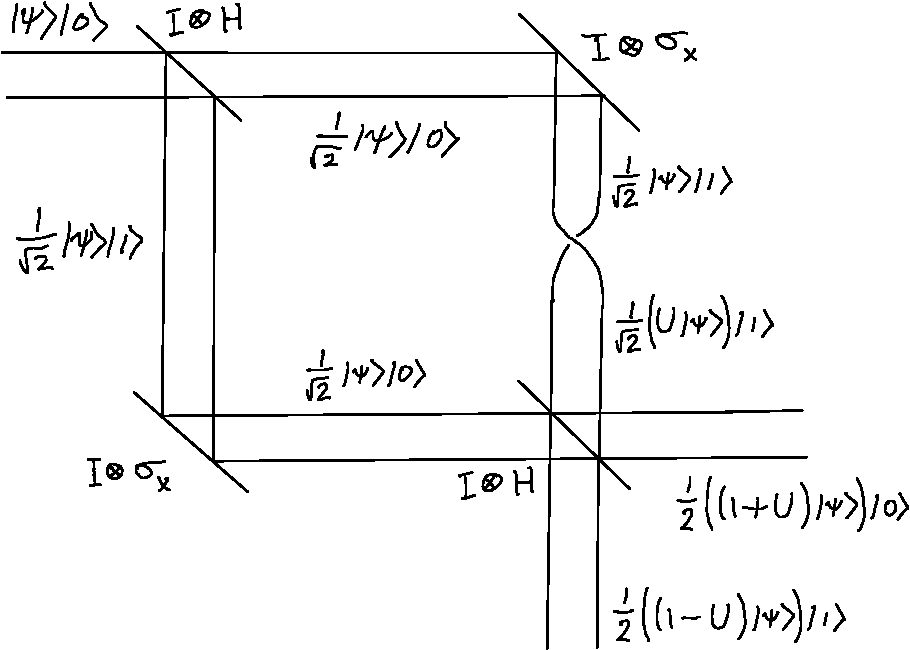
\includegraphics[width=0.8\textwidth]{img/exchange-interference-cropped.png}
  \caption{Schematic of a quantum circuit to measure the exchange operator $U$ via interference. TODO: Fix $H ↦ I⊗H$ and rotate the final mirror.}
  \label{fig:exchange interference}
\end{figure}

Let $\mathcal{H}_A$ be the Hilbert space of the two anyons and let $|0⟩$ and $|1⟩$ be two orthonormal states, spanning the Hilbert space $\mathcal{H}_B$, in \cref{fig:exchange interference} they represent horizontal and vertical propagation, respectively. Thus, the total Hilbert space is $\mathcal{H} = \mathcal{H}_A⊗\mathcal{H}_B$.

The Hadamard transform defined as
\begin{equation}
  \begin{aligned}
    H : \quad
    \begin{aligned}
      |0⟩ &↦ \tfrac{1}{\sqrt{2}}\big(|0⟩+|1⟩\big) \\
      |1⟩ &↦ \tfrac{1}{\sqrt{2}}\big(|0⟩-|1⟩\big)
    \end{aligned}
  \end{aligned}
\end{equation}
is a unitary transform that forms a superposition of states. Apply the Hadamard transform to the initial state
\begin{equation}
  |ψ⟩⊗|0⟩ \xmapsto{I⊗H} \frac{1}{\sqrt{2}} \Big( |ψ⟩⊗|0⟩ + |ψ⟩⊗|1⟩ \Big).
\end{equation}
Next, apply the unitary operator
\begin{equation}
  \widetilde{U} : \quad
  \begin{alignedat}{4}
    |ψ⟩⊗|0⟩ &{}↦{}& |ψ⟩\phantom{)}&⊗|0⟩ \\
    |ψ⟩⊗|1⟩ &{}↦{}& (U|ψ⟩)&⊗|1⟩
  \end{alignedat}
\end{equation}
that exchanges the particles if they are in the $|1⟩$ state. Note that in \cref{fig:exchange interference} we needed the $I⊗σₓ$ operator where
\begin{equation}
  σₓ : \quad
  \begin{aligned}
    |0⟩ &↦ |1⟩ \\
    |1⟩ &↦ |0⟩
  \end{aligned}
\end{equation}
to recombine the states after the split, this is only for the schematic, mathematically it can be ignored since $σₓ$ simply flips the $|0⟩$ and $|1⟩$ states. The state is thus mapped to
\begin{equation}
  \frac{1}{\sqrt{2}} \Big( |ψ⟩⊗|0⟩ + (U|ψ⟩)⊗|1⟩ \Big).
\end{equation}
Finally, perform a Hadamard transform again, mapping the state to
\begin{equation}
  \frac{1}{2} \Big( \big((I+U)|ψ⟩\big)⊗|0⟩ + \big((I-U)|ψ⟩\big)⊗|1⟩ \Big).
\end{equation}
To sum up we have performed the sequence of three operations $(I⊗H)\widetilde{U}(I⊗H)$. Note that if $U = I$ this sequence of operations does nothing, since $H² = I$.

The exchange phase $U$ can now be measured by performing a measurement in the $\mathcal{H}_B$ space. In the abelian case $U = e^{iθ}$ and the probability of measuring the final state to be in the state $|0⟩$ is
\begin{equation}
  \begin{aligned}
    \abs*{\frac{1+U}{2}}^2
    &= \abs*{\frac{1+e^{iθ}}{2}}^2 \\
    &= \frac{1}{4} \left( 1+e^{iθ} \right) \left( 1+e^{iθ} \right)^* \\
    &= \frac{1}{4} \left( 1 + e^{iθ}e^{-iθ} + e^{iθ} + e^{-iθ} \right) \\
    &= \frac{1}{4} \left( 2 + 2\cos(θ) \right) \\
    &= \frac{1}{2} \left( 1 + \cos(θ) \right).
  \end{aligned}
\end{equation}
The anyonic phase $θ$ can thus be measured, and in this setup $θ$ can be understood as a shift of the probability of measuring the final state in $|0⟩$ or $|1⟩$. In particular, bosons ($θ=0$) always end up in $|0⟩$ and fermions ($θ=π$) always end up in $|1⟩$.

In the case where $U$ is non-abelian, computing the probability of measuring the final state in $|0⟩$ becomes more involved because $U$ can no longer be moved between the two Hilbert spaces $\mathcal{H}_A$ and $\mathcal{H}_B$ as in the case where $U$ is abelian (in which case $U$ is a scalar). We need some more machinery for this, namely that of density operators and partial trace. These concepts are discussed in \cref{sec:density operators and partial trace}. This unfortunate forward reference allows the discussion of quantum computation in \cref{sec:intro qc} to be self-contained.

Denote the resulting state by
\begin{equation}
  |Ψ⟩ = \frac{1}{2} \Big( \big((I+U)|ψ⟩\big)⊗|0⟩ + \big((I-U)|ψ⟩\big)⊗|1⟩ \Big)
\end{equation}
and form the corresponding density operator
\begin{equation}
  ρ_ψ = |ψ⟩⟨ψ|.
\end{equation}
We measure the interference by measuring the probability $P(|0⟩)$ that $ρ_ψ$ is in the state $|0⟩$ in subsystem $B$. The available information of the total state $ρ_ψ$ in subsystem $B$ is given by the reduced density operator $ρ_ψᴮ$ with subsystem $A$ traced out, defined in \cref{eq:red dens op}. Thus,
\begin{equation}
  P(|0⟩) = ⟨0|ρ_ψᴮ|0⟩.
\end{equation}
We have
\begin{equation}
  \begin{aligned}
    ρ_ψ = |Ψ⟩⟨Ψ| =
    \frac{1}{4} \Bigg(
      & \bigg[(I+U)|ψ⟩⟨ψ|(I+U^*)\bigg] ⊗ |0⟩⟨0| {}+{} \\
      & \bigg[(I-U)|ψ⟩⟨ψ|(I-U^*)\bigg] ⊗ |1⟩⟨1| {}+{} \\
      & \bigg[(I+U)|ψ⟩⟨ψ|(I-U^*)\bigg] ⊗ |0⟩⟨1| {}+{} \\
      & \bigg[(I-U)|ψ⟩⟨ψ|(I+U^*)\bigg] ⊗ |1⟩⟨0|
    \Bigg).
  \end{aligned}
\end{equation}
Thus
\begin{equation}
  \begin{aligned}
    ⟨0|ρ_ψᴮ|0⟩_B
    &= \frac{1}{4} \operatorname{tr} \Big[(I+U)|ψ⟩⟨ψ|(I+U^*)\Big] \\
    &= \frac{1}{4} ∑ₖ ⟨k|(I+U)|ψ⟩⟨ψ|(I+U^*)|k⟩ \\
    &= \frac{1}{4} ∑ₖ |⟨k|(I+U)|ψ⟩|².
  \end{aligned}
\end{equation}

We recover the result for abelian anyons by letting $U = e^{iθ}$,
\begin{equation}
  \begin{aligned}
    ⟨0|ρ_ψᴮ|0⟩_B
    &= \frac{1}{4} ∑ₖ |⟨k|(I+U)|ψ⟩|² \\
    &= \frac{1}{4} ∑ₖ |1+e^{iθ}|² |⟨k|ψ⟩|² \\
    &= \frac{1}{2} (1+\cosθ),
  \end{aligned}
\end{equation}
where $∑ₖ |⟨k|ψ⟩|² = 1$ due to normalization of $|ψ⟩$.

For general $U$ it is difficult to say much more than this. The dependence of the probability $⟨0|ρ_ψᴮ|0⟩$ on the exchange operator $U$ can be rather involved. Assuming that we have control of the state $|ψ⟩$, with an appropriate set of choices for $|ψ⟩$ the elements of $U$ can be deduced by repeating the interference measurement. We outline this idea in the following example.

\begin{example}
  Let $ℋ_A$ be two-dimensional. We can then write
  \begin{equation}
    |ψ⟩ = c₀|0⟩ + c₁|1⟩
  \end{equation}
  and
  \begin{equation}
    U =
    \begin{pmatrix}
      u_{00} & u_{01} \\
      u_{10} & u_{11}
    \end{pmatrix}
    =
    \begin{pmatrix}
      a & b \\
      -e^{iθ}b^* & e^{iθ}a^*
    \end{pmatrix}
  \end{equation}
  Thus we have
  \begin{equation}
    \begin{aligned}
      ⟨0|ρ_ψᴮ|0⟩_B
      &= \frac{1}{4} \left( |(u_{00}+1)c₀ + u_{01}c₁|² + |u_{10}c₀ + (u_{11}+1)c₁|² \right) \\
      &= \frac{1}{4} \left( |(a+1)c₀ + bc₁|² + |-e^{iθ}b^*c₀ + (e^{iθ}a^*+1)c₁|² \right).
    \end{aligned}
  \end{equation}
  Determining $U$ amounts to determining four real parameters, $\operatorname{arg}(a)$, $\operatorname{arg}(b)$, $|a|$ and $θ$. For example, the choice $|ψ⟩=|0⟩$ gives
  \begin{equation}
    \begin{aligned}
      ⟨0|ρ_ψᴮ|0⟩_B
      &= \frac{1}{4} \left( |a+1|² + |-e^{iθ}b|² \right) \\
      &= \frac{1}{4} \left( |a|² + 1 + 2\operatorname{Re}(a) + |b|² \right) \\
      &= \frac{1}{2} \left( 1 + \cos(\operatorname{arg}(a)) \right),
    \end{aligned}
  \end{equation}
  allowing measurements of $\operatorname{arg}(a)$.
  Similarly, the other parameters of $U$ can be determined by appropriately choosing the state $|ψ⟩$.

  If we work in the eigenbasis of $U$ we have
  \begin{equation}
    U =
    \begin{pmatrix}
      e^{iθ₁} & 0 \\
      0 & e^{iθ₂}
    \end{pmatrix}
  \end{equation}
  and then
  \begin{equation}
    ⟨0|ρ_ψᴮ|0⟩_B = \frac{1}{2} \left( |c₀|²(1+\cos(θ₁)) + |c₁|²(1+\cos(θ₂)) \right).
  \end{equation}
\end{example}

This procedure can be straight-forward extended to let the the state $|ψ⟩$ represent more than two anyons, and thus allow the operator $\widetilde{U}$ to introduce a more complex braid. In this way, truly non-abelian properties of a larger system of anyons can in principle be probed.

Other methods of anyonic interferometry is discussed in \cite{bonderson}. Note that as one anyon is taken around one or several other anyons, the introduced phase can only be measured after one full loop as been traversed and the phase can be compared to another anyon. Thus, it is not physical to say that the phase continuously (or in any other way) changes during the exchange. That is, how the phase is affected before the particles meet is non-physical, we are free to choose this as long as the choice respects the result of a complete winding of particles; this illustrates the gauge invariance of the anyonic phase during braiding.









































\section{Anyon models and physical realizability}\label{sec:models and realizability}

This thesis focuses primarily on the mathematical aspects of anyons, however, in this section we give a short account of possible physical realizations for anyons. This topic is further discussed in for instance \cite{nayak,topological quantum compiling,slingerland bais}.

Abelian anyons have been claimed to have been detected in the fractional quantum hall (FQH) effect \cite{abelian fqh}. These results are not unambiguous and total consensus does not exist in the scientific community. It is  Furthermore, it has only been conjectured that non-abelian anyons can be realized in FQH liquids at the filling fractions $\nu = 5/2$, where anyons known as the Ising anyons are thought to exist \cite{wang book}. Partial experimental results exist which support the existence of non-abelian anyons \cite{non-abelian experimental}. The Fibonacci anyon model which is studied in \cref{fibonacci anyons} has support from the topological quantum field theory $SU(2)₃$ Chern-Simons-Witten (CSW). \cite{nayak}

There are different attempts to identify whether particles obey anyonic statistics. Interferometry methods have been developed, as in \cite{bonderson}. Another approach is to study the wave function density, as outlined in \cite{lundholm-rougerie,fractional angular momentum}. An unambiguous argument for abelian anyons in the context of FQH is given in \cite{lundholm-rougerie}. The benefit of using interferometry is that it is a direct way to identify braid statistics, while the wave function density is an indirect effect of the statistics. However, anyonic interferometry is in practice difficult to achieve, it can be argued that wave function density is easier to measure.

In the literature one generally encounters two types of anyons.
\begin{enumerate}
  \item Anyons with quantum dynamics, giving rise to anyonic particle statistics, i.e.\ braid statistics. Such particles must necessarily be allowed to move freely in space, such as in a gas. This is the type of anyons that one has in mind when discussion statistical repulsion.
  \item Anyons with fixed or controlled coordinates. In the strict sense this can be any quantum system that is governed by a representation of the braid group. This is the type of anyons that one has in mind when discussing the use of anyons for topological quantum computation. The anyons need to be fixed so that controlled braiding can be performed. In principle this can be achieved by forcing the position of dynamical anyons by placing each anyon in a deep potential that can be externally controlled.
\end{enumerate}

%!TEX root = nonabelions.tex

\chapter{Statistical repulsion}\label{chap:statistical repulsion}

In this chapter we give a lower bound for the kinetic energy of free anyons. This gives rise to what is known as statistical repulsion, an essentially geometric effect of the exchange operator that causes an effective repulsion of indistinguishable particles. This has consequences for the density of the wave function, and might thus be measured. This chapter is in part based on \cite{methmmp,lundholm-solovej,mancarella}. See also \cite{larson-lundholm} for the case of what is known as extended abelian anyons.


A quantum system is generally determined by a Hamiltonian $\hat{H} = \hat{T} + \hat{V}$ where $\hat{T} = \hat{p}⋅\hat{p} = -∇²$ is the kinetic energy operator, $\hat{p} = -i∇$ is the momentum operator, and $\hat{V}$ is the potential energy operator. We shall consider free particles, i.e.\ $\hat{V} = 0.$






\section{Fermionic statistical repulsion}

Recall that the exchange operator is the braid group representation of a simple exchange of particles. In the case of bosons and fermions in $d ≥ 3$ dimensions the exchange operator is simply the identity and $-1$, respectively. That is,
\begin{equation}
  ψ(x_2, x₁) = \pm ψ(x₁, x_2).
\end{equation}
For fermions, this leads to the well-known Pauli exclusion principle. Simply stated, if $x₁ = x_2$ it immediately follows that $ψ(x₁, x₁) = 0$, the particles cannot occupy the same position. More generally, the anti-symmetry of the fermionic wave function causes the kinetic energy to increase as the particles tend closer to each other. This is an effective repulsion due to the particle statistics. We shall now see this in more detail.

Consider $n$ indistinguishable particles on $ℝᵈ$. Let $x₁, …, x_n$ be the coordinates of the particles, i.e.\ $xⱼ ∈ ℝᵈ$. This collection of particles is described by an $n$-particle wave function $ψ(x₁, …, x_n) ∈ L^2(ℝ^{dn})$, i.e.\ a square integrable complex-valued function on $ℝ^{dn}$. The kinetic energy $T$ of this system is defined as
\begin{equation}
  T ≔ ⟨ψ|\hat{T}|ψ⟩ = ∑_{j=1}^n ∫_{ℝ^{dn}} |∇ⱼ ψ|^2 dx.
\end{equation}
In the present discussion we shall assume that $ψ$ is normalized and in the domain of the operator. A detailed discussion for abelian anyons can be found in \cite{larson-lundholm} and \cite{lundholm-solovejAHP}, see also \cite{dellantonio}.

Let the particles be fermions, i.e.\ $ψ ∈ L_\text{asym}^2(ℝ^{dn})$. This is the subspace of functions $ψ$ in $L^2(ℝ^{dn})$ such that $ψ(…, xⱼ, …, xₖ, …) = - ψ(…, xₖ, …, xⱼ, …)$ for $j \ne k$. In this case, we have the following theorem \cite{hoholt,methmmp}.

\begin{theorem}[Many-body Hardy inequality for fermions]\label{thm:hardy fermion}
  In the described setting with $ψ$ being an $n$-particle fermionic wave function, the following lower bound for the kinetic energy holds
  \begin{equation}\label{eq:fermion ineq}
    ∫_{ℝ^{dn}} ∑_{j=1}^n |∇ⱼψ|^2 dx \ge
    \frac{d²}{n} ∫_{ℝ^{dn}} ∑_{1≤j<k≤n} \frac{|ψ|^2}{|xⱼ-xₖ|^2} dx +
    \frac{1}{n} ∫_{ℝ^{dn}} \left|∑_{j=1}^n ∇ⱼ ψ \right|^2 dx.
  \end{equation}
\end{theorem}

The first integral shows that fermionic particles have an inverse-squared pairwise effective repulsion. The second integral on the right-hand side essentially gives the contribution of the motion of the center of mass.

We give an outline of the proof.

\begin{proof}
  First, one can show
  \begin{equation}
    ∑_{j=1}^n |∇ⱼ ψ|^2 = \frac{1}{n} ∑_{1 \le j < k \le n} \left| (∇ⱼ - ∇ₖ) ψ \right|^2 + \frac{1}{n} \left| ∑_{j=1}^n ∇ⱼ ψ \right|²,
  \end{equation}
  by expanding the expression, known as the many-body parallelogram identity. The last term sum to the center of mass motion and is not of interest. We focus on the first sum on the right-hand side.

  Introduce relative coordinates for each pair $(j,k)$ of particles,
  \begin{equation}
    \begin{aligned}
      x_{jk}^\text{rel} &≔ (xⱼ - xₖ)/2, & x_{jk}^\text{cm} &≔ (xⱼ + xₖ)/2, \\
      ∇_{x_{jk}^\text{rel}} &≔ ∇ⱼ - ∇ₖ, & ∇_{x_{jk}^\text{cm}} &≔ ∇ⱼ + ∇ₖ.
    \end{aligned}
  \end{equation}
  It shall be useful to split the coordinates as $x = (xⱼ, xₖ; x')$ where $x' ∈ ℝ^{d(n-2)}$ and $j < k$ fixed. Next, define the relative wave function
  \begin{equation}
    u(x_{jk}^\text{rel}, x_{jk}^\text{cm}) ≔ ψ(x₁, …, xⱼ=x_{jk}^\text{cm}+x_{jk}^\text{rel}, …, xₖ = x_{jk}^\text{cm}-x_{jk}^\text{rel}, …, x_n).
  \end{equation}
  We then have $u(-x_{jk}^\text{rel}, x_{jk}^\text{cm}) = -u(x_{jk}^\text{rel}, x_{jk}^\text{cm})$ for fermions, by the anti-symmetry of $ψ$.

  With this change of variables we have
  \begin{equation}
    \begin{aligned}
      ∫_{ℝ^{dn}} \left|(∇ⱼ-∇ₖ)ψ\right|^2 dx
      &= ∫_{ℝ^{d(n-2)}} ∫_{ℝᵈ \times ℝᵈ} \left|(∇ⱼ-∇ₖ)ψ\right|^2 dxⱼdxₖdx' \\
      &= ∫_{ℝ^{d(n-2)}} ∫_{ℝᵈ \times ℝᵈ} \left|∇_{x_{jk}^\text{rel}}u\right|^2  2 dx_{jk}^\text{rel}dx_{jk}^\text{cm} dx'.
    \end{aligned}
  \end{equation}

  Finally, one shows, for anti-symmetric (fermionic) wave functions,
  \begin{equation}
    ∫_{ℝᵈ} \left|∇_{x_{jk}^\text{rel}} u \right|^2 dx_{jk}^\text{rel} \ge \frac{d^2}{4} ∫_{ℝᵈ} \frac{|u|^2}{|x_{jk}^\text{rel}|^2} dx_{jk}^\text{rel}
  \end{equation}
  from which the result follows.
\end{proof}

In the outline of the proof we skipped the details of the last step. To obtain a similar inequality for anyons, it is exactly this step that shall be important, and we now look into this in more detail in the case $d = 2$.














\section{Anyonic statistical repulsion}

In the proof outline of \cref{thm:hardy fermion}, the assumption that $ψ$ is anti-symmetric is used only in the last step where the expression
\begin{equation}
  ∫_{ℝᵈ} \left|∇_{x_{jk}^\text{rel}} u(x) \right|^2 dx_{jk}^\text{rel}
\end{equation}
is considered. We now extend this to the more general case with
\begin{equation}\label{eq:rel boundary cond}
  u(-x_{jk}^\text{rel}, x_{jk}^\text{cm}) = U_γ u(x_{jk}^\text{rel}, x_{jk}^\text{cm})
\end{equation}
for general anyons with simple exchange represented by $U_γ$. This implicitly assumes $d = 2$ so that $U_γ$ determines braid statistics. Generally, $U_γ$ may denote simple exchange around a number of inner anyons, i.e.\ $γ$ denotes a loop in configuration space, enclosing a number of fixed anyons. We shall return to the details of this later.

In polar coordinates $x_{jk}^\text{rel} = (r, φ)$ we have
\begin{equation}
  ∫_{ℝ²} \left|∇_{x_{jk}^\text{rel}} u \right|^2 dx_{jk}^\text{rel} =
  ∫_{r=0}^∞ ∫_{φ=0}^{2π} \left( \left|∂ᵣu\right|^2 + \frac{\left|∂_φu\right|²}{r²} \right) r dφ dr.
\end{equation}
It is the angular derivative term that gives the contribution of the exchange statistics. Thus, we only consider this integral
\begin{equation}
  ∫₀^{2π} \left|∂_φu\right|² dφ.
\end{equation}
Since we consider $r$ fixed, we define $u(φ) ≔ u(r,φ)$. In this way, the loop $γ = γᵣ$ is determined by $r$ and the number of encircled fixed anyons varies with $r$. Loops with different number of encircled fixed anyons are not homotopically equivalent and thus the exchange operator $U_{γᵣ}$ depends on $r$. The boundary condition \cref{eq:rel boundary cond} may thus be written as $u(π) = U_{γᵣ} u(0)$. Furthermore,
\begin{equation}
  \begin{aligned}
    ∫₀^{2π} \left|∂_φu\right|² dφ
    &=
    ∫₀^π \left|∂_φu(φ)\right|² dφ +
    ∫₀^π \left|∂_φu(π+φ)\right|² dφ \\
    &=
    ∫₀^π \left|∂_φu(φ)\right|² dφ +
    ∫₀^π \left|∂_φU_{γᵣ}u(φ)\right|² dφ \\
    &=
    2∫₀^π \left|∂_φu\right|² dφ
  \end{aligned}
\end{equation}
since unitary operators are norm preserving.

Define the operator
\begin{equation}\label{eq:D}
  D = -i∂_φ, \quad \operatorname{Dom}D = \{u : u, ∂_φ u ∈ L²([0,π]), u(π) = U_{γᵣ}u(0)\}.
\end{equation}
The expectation value of $D²$ with $\operatorname{dom} D² = \{ u : u, Du ∈ \operatorname{dom}D \}$,
\begin{equation}
  \begin{aligned}
    ⟨u|D²|u⟩
    &= -∫₀^π \overline{u} ∂_φ² u \,dφ \\
    &= -\overline{u}∂_φu\Big|₀^π + ∫₀^π ∂_φ\overline{u} ∂_φ u \,dφ \\
    &= ∫₀^π ∂_φ\overline{u} ∂_φ u \,dφ \\
    &= ∫₀^π |∂_φu|² dφ
  \end{aligned}
\end{equation}
is precisely the integral we are considering. In the above calculation, the boundary term vanishes since $U_{γᵣ}$ is unitary,
\begin{equation}
  \begin{aligned}
    \overline{u}∂_φu\Big|₀^π
    &= \overline{u}(π)∂_φu(π) - \overline{u}(0)∂_φu(0) \\
    &= U_{γᵣ}^*\overline{u}(0)U_{γᵣ}∂_φu(0) - \overline{u}(0)∂_φu(0) \\
    &= (U_{γᵣ}^*U_{γᵣ} - I)\overline{u}(0)∂_φu(0) \\
    &= 0.
  \end{aligned}
\end{equation}
Similarly, one shows that $D$ is self-adjoint. Thus, also $D²$ is self-adjoint, so the Rayleigh quotient of $D²$ can be used to obtain a lower bound by the min-max theorem,
\begin{equation}
  ∫₀^π |∂_φu|² dφ = ⟨u|D²|u⟩ ≥ \inf σ(D²) ≕ λ_{0,γᵣ}²,
\end{equation}
where we assume that $u$ is normalized in $L²[0,π]$.

By the spectral theorem we have
\begin{equation}
  σ(D²) = \{λ² : λ ∈ σ(D)\}
\end{equation}
The spectrum of $D$ is straight forward to compute.

\begin{lemma}
  The spectrum of $D$ is given by
  \begin{equation}
    σ(D) = \{ λ : e^{iλπ} \text{ is an eigenvalue of $U_{γᵣ}$} \}
  \end{equation}
\end{lemma}
\begin{proof}
  The eigenequation for $D$ gives
  \begin{equation}
    Du = λu ⟺ -iu' = λu ⟺ u(φ) = C e^{iλφ}
  \end{equation}
  for a non-zero constant vector $C ∈ ℂᵏ$. Moreover, the boundary condition \cref{eq:D} implies
  \begin{equation}
    u(π) = U_{γᵣ} u(0) ⟹ Ce^{iλπ} = U_{γᵣ}C,
  \end{equation}
  i.e.\ $e^{iλπ}$ is an eigenvalue of $U_{γᵣ}$, with eigenvector $C$.
\end{proof}

Thus, we have a lower bound for the angular term, carrying the contribution of the anyonic statistics leading to statistical repulsion.

\begin{theorem}\label{thm:inf spec bound}
  Anyons with exchange operator $U_{γᵣ}$ satisfy the inequality
  \begin{equation}
    ∫₀^π |∂_φu|² dφ ≥ \inf \, \{ λ² : e^{iλπ} \text{ is an eigenvalue of $U_{γᵣ}$} \} = λ_{0,γᵣ}².
  \end{equation}
\end{theorem}

\begin{remark}
  Each eigenvalue of $U_{γᵣ}$ is on the form $e^{iαπ}$ with $0≤α<2$ since $U_{γᵣ}$ is unitary. By the theorem, each eigenvalue gives rise to a family of possible energy levels
  \begin{equation}
    \{ (α+2q)² : q ∈ ℤ \}
  \end{equation}
  for the angular Hamiltonian $H = D²$, with corresponding eigenfunctions
  \begin{equation}
    u_q(φ) = C₁e^{i(α+2q)φ}.\qedhere
  \end{equation}
\end{remark}


\begin{remark}
  Instead of introducing anyonic exchange as the condition $u(π) = U_{γᵣ} u(0)$ one can use the framework of fiber bundles to model anyons by changing the kinetic energy operator from
  \begin{flalign}
    &\text{\textit{Anyon gauge:}} & \widehat{T} &= ∑_{j=1}^n -∇ⱼ^2 &
  \intertext{to}
    &\text{\textit{Magnetic gauge:}} & \widehat{T}_A &= ∑_{j=1}^n \left( -i ∇ⱼ + Aⱼ \right)^2,&
  \end{flalign}
  where $A$ is a connection one-form on the bundle of which the wave function is a section. In this way the wave function may be chosen periodic $u(π)=u(0)$, i.e.\ the anyonic exchange is then completely captured by $Aⱼ$ and $ψ$ is bosonic \cite{nakahara}.
  % TODO: The following example illustrates this.
  % \begin{example}
  %   Skriv ner fr. tidigare anteckningar: Två abelska anyoner. Connection $Aⱼ = α ∑_{j≠k} \frac{(xⱼ-xₖ)^⟂}{|xⱼ-xₖ|²}$.
  % \end{example}
\end{remark}
















\section{Separating the state space}

In the above discussion, the exchange operator $U_{γᵣ}$ is defined to be a simple exchange of the pair $(xⱼ,xₖ)$, possibly around $p$ other anyons. We started by considering the expression
\begin{equation}
  ∫_{ℝ^{2(n-2)}} ∫_{ℝ² \times ℝ²} \left|∇_{x_{jk}^\text{rel}}u\right|^2  2 dx_{jk}^\text{rel}dx_{jk}^\text{cm} dx'.
\end{equation}
The inner integral concerns anyons $j$ and $k$ with the remaining $n-2$ considered fixed. The inner integral is rewritten as
\begin{equation}
  \begin{aligned}
    ∫_{ℝ²} \left|∇_{x_{jk}^\text{rel}} u \right|^2 dx_{jk}^\text{rel}
    &= ∫_{r=0}^∞ ∫_{φ=0}^{2π} \left( \left|∂ᵣu\right|^2 + \frac{\left|∂_φu\right|²}{r²} \right) r dφ dr \\
    &≥ ∫_{r=0}^∞ ∫_{φ=0}^{2π} \left( \left|∂ᵣu\right|^2 + λ_{0,γᵣ}²\frac{\left|u\right|²}{r²} \right) r dφ dr
  \end{aligned}
\end{equation}
and we assume $u$ satisfies the anyonic boundary condition $u(π) = U_{γᵣ} u(0)$. The exchange operator $U_{γᵣ}$ may depend on $r$ since the number of encircled anyons in the loop $γᵣ$ may affect the exchange operator $U_{γᵣ}$. To make this precise we separate the state space into open annuli (regions between two concentric circles) centered at $x_{jk}^\text{cm}$, such that none of the fixed $n-2$ anyons are at the interior of an annulus, cf.\ \cref{fig:annuli}. This gives a separation of $ℝ^2$ into regions with increasing number $p$ of the $n-2$ fixed anyons. Let $r₁ \le r₂ \le … \le r_{n-2}$ be the radial coordinate of the $n-2$ fixed anyons. The innermost annulus is an open disk (degenerate annulus) with radius $r₁$, the second innermost annulus is the region between circles of radius $r₁$ and $r_2$, etc. Note that the circles with radii $r₁, r₂, …, r_{n-2}$ are not contained in any annuli, since the anyons cannot pass through each other, and we are considering angular motion. If the radii of two fixed anyons coincide, then there is no annulus separating them. The removal of these circles removes more points than $\bbDelta$, however this is no issue since the circles of radius $rⱼ$ have measure zero.

In this way, exchange of particles $j$ and $k$ depend on $r$, i.e.\ $U_{γᵣ} = U_{γᵣ}(r)$. Since the dependence on $r$ is exclusively due to the $p$ number of encircled fixed anyons, we introduce the notation
\begin{equation}
  Uₚ ≔ U_{γᵣ}(r), \quad r_{p-1} < r < rₚ,
\end{equation}
with $r₀ = 0$ and $r_{n-1} = ∞$. This is precisely the exchange braid introduced in \cref{def:exchange braid}. The exchange corresponding to $Uₚ$ is visualized in \cref{fig:Up exchange}.

\begin{figure}[h]
  \centering
  \begin{tikzpicture}[scale=0.8]
    \draw[->] (-3.75,0) -- (3.75,0) node[below] {$x$};
    \draw[->] (0,-3.75) -- (0,3.75) node[right] {$y$};
    \draw (0,0) circle (1.25);
    \draw (0,0) circle (2);
    \draw (0,0) circle (3);
    \node at (0.55, 0.35) {$p = 0$};
    \node at (0.55, 1.5) {$p = 1$};
    \node at (0.55, 2.375) {$p = 2$};
    \node at (0.55, 3.25) {$p = 3$};
    \node at ({1.25*cos(220)}, {1.25*sin(220)}) {$\bullet$};
    \node at ({2*cos(130)}, {2*sin(130)}) {$\bullet$};
    \node at ({3*cos(-55)}, {3*sin(-55)}) {$\bullet$};
    \node at (1.5, -0.2) {$r₁$};
    \node at (2.25, -0.2) {$r_2$};
    \node at (3.25, -0.2) {$r_3$};
  \end{tikzpicture}
  \caption{Illustration of annuli separating $ℝ^2$ into regions with increasing number $p$ of contained anyons. A blob $\bullet$ denotes a fixed anyon. In each annulus, exchange of the two free anyons, i.e.\ as $φ$ increases from $0$ to $π$, a given number $p$ of fixed anyons will be encircled.}
  \label{fig:annuli}
\end{figure}

\begin{figure}[h]
  \centering
  \includegraphics{img/interchange_loop_p.pdf}
  \caption{Exchange of a pair of anyons around $p$ fixed anyons. Figure taken from \cite{lundholm-solovej}.}
  \label{fig:Up exchange}
\end{figure}








\subsection{Abelian anyons}\label{sec:statistical repulsion abelian ayons}

Abelian anyons have an exchange operator on the form $U₀ = e^{iαπ}$ for $0≤α<2π$. Moreover, by \cref{res:abelian repr} every simple exchange is determined by the same representation. Thus,
\begin{equation}
  Uₚ = ρ(σ₁)ρ(σ₂)⋯ρ(σₚ)ρ(σ_{p+1})ρ(σₚ)⋯ρ(σ₂)ρ(σ₁) = e^{i(2p+1)απ}.
\end{equation}
In this case, the spectrum for $D²$ is given by
\begin{equation}
  σ(D²) = \{ \left( (2p+1)α + 2q \right)² : q ∈ ℤ \}
\end{equation}
and thus \cref{thm:inf spec bound} yields the following result for $n → ∞$.

\begin{theorem}
  Abelian anyons with exchange operator $U₀ = e^{iαπ}$ satisfy the lower bound
  \begin{equation}
    \begin{gathered}
      ∫₀^π |∂_φu|² dφ ≥ λ_{0,γᵣ}² = \\
      % \inf_{p,q ∈ ℤ} \left( (1+2p)α + 2q \right)² = \\
      = \begin{cases}
        \frac{1}{ν^2}, & \text{if $α = \frac{μ}{ν}$ with $μ ∈ ℤ, ν ∈ ℕ₊$ relatively prime and $μ$ odd}, \\
        0, & \text{otherwise}
      \end{cases}
    \end{gathered}
  \end{equation}
\end{theorem}

The last equality in the theorem is essentially a number-theoretic result, proved in proposition 5 in \cite{lundholm-solovej}.

From this we have an immediate corollary for bosons ($α = 0$) and fermions ($α = 1$).

\begin{corollary}
  With $α = 0$, the exchange operator is
  \begin{equation}
    U_p = e^{i(1+2p)απ} = 1
  \end{equation}
  for all $p$, i.e.\ bosons do not ``see'' each other, and they have no statistical repulsion; $\inf σ(D²) = 0$.

  With $α = 1$, the exchange operator is
  \begin{equation}
    U_p = e^{i(2p+1)απ} = -1
  \end{equation}
  for all $p$, i.e.\ fermions do not ``see'' the encircled $p$ fermions. However, the particles in the exchange pair do ``see'' each other, in the sense that their wave function changes sign after they have been exchanged, as expected. This gives a non-zero statistical repulsion, $\inf σ(D²) = λ_{0,γᵣ}² = 1$ for all $γᵣ$.
\end{corollary}

The effects of the statistical repulsion may have consequences for the wave function density, e.g. the wave function may be forced to vanish on $\bbDelta$; as particles get close to each other. As we have discussed, the density may be measured. Thus, understanding the effects of the statistical repulsion may help in the experimental search for anyons. It may also affect the free energy and the stability of anyonic many-body systems, see \cite{lundholm-solovej,many-anyon trial states,lundholm-solovejAHP}.






\subsection{Non-abelian anyons}

The exchange operator $Uₚ$ of non-abelian anyons cannot be characterized in a straight forward way as for abelian anyons, essentially due to $ρ(σⱼ)$ and $ρ(σ_{j+1})$ not commuting. Because of this, determining the spectrum $σ(Uₚ)$ and thus the lower bound
\begin{equation}
    ∫₀^π |∂_φu|² dφ ≥ λ_{0,γᵣ}² = \inf \, \{ λ² : e^{iλπ} ∈ σ(Uₚ) \},
\end{equation}
becomes problematic. In light of this, we must better understand how the non-abelian exchange operator $Uₚ$ arises. To do this, we introduce the general framework of abstract anyon models in the following chapter. First we make the following general observation.

\begin{remark}
  The abelian part of $U ∈ U(k)$, i.e.\ the $U(1)$ part in the factorization $U(k) = U(1) × SU(k)$, is given by $e^{iθ}$ such that
  \begin{equation}
    U = e^{iθ} U₀
  \end{equation}
  where $\det U₀ = 1$. Note the relation
  \begin{equation}
    \det U = \det(e^{iθ}U_0) = e^{ikθ}.
  \end{equation}
  Varying the abelian phase $θ$ can be seen as shifting the eigenvalues of $U$ uniformly along the complex unit circle. In particular, with $U₀$ diagonalized as $U₀ = \operatorname{diag}(e^{iθ₁}, …, e^{iθₖ})$, changing the abelian phase according to $e^{iθ} ↦ e^{-iθⱼ}$ gives $U$ a zero eigenvalue. Thus, implying zero statistical repulsion. However, the abelian part can generally not be decoupled and controlled independently.
\end{remark}

%!TEX root = nonabelions.tex

\chapter{Abstract anyon models}\label{anyon models}

In this chapter we shall present the framework of abstract anyon models, leading up to the succeeding chapter that characterizes braiding of anyons described by abstract anyon models.

Anyon models can be modeled by unitary braided tensor categories, see \cite{kitaev,naaijkens,prakash,tensor categories,tuba}. However, setting up this framework in full generality is redundant for our purposes and we take a more straight forward approach, which is also most common in the literature. The benefit of the categorical approach is that consistency of braiding and fusion is most naturally shown this way. We shall see the ties between the straight forward approach and the categorical model when discussing the consistency conditions in \cref{sec:pentagon hexagon}.

This chapter is in part based on \cite{preskill,kitaev,bonderson}. We shall be using the notation that is standard in the literature, and when possible make use of and extend the fusion diagram notation, which greatly clarifies braiding of fusion states.

Starting with \cref{sec:anyonic braid representations in fusion space} we show how a given abstract anyon model gives rise to representations of the braid group.

\section{Preliminaries}

An abstract anyon model consists of a set of labels representing different types of anyons. These labels are known as anyonic charge, topological charge or superselection labels. Anyons can be combined, or fused, to give an anyon of some charge, possibly in different ways. This is modeled by a fusion algebra
\begin{equation}
  a \times b = \sum_c N_{ab}^c c
\end{equation}
representing the possible outcomes from fusion of anyons of type $a$ and $b$. The fusion multiplicities $N_{ab}^c$ are non-negative integers denoting the number of distinct ways $a$ and $b$ can fuse to $c$. In each anyon model there is the trivial label $1$, representing the vacuum, with the property $N_{a1}^b = N_{1a}^b = \delta_{ab}$, i.e.\ $1$ fuses trivially with every other charge. Furthermore, to each charge $a$ there is a corresponding conjugate charge $\bar{a}$ representing the antiparticle of $a$, with the property $N_{ab}^1 = \delta_{b\bar{a}}$, i.e.\ $a$ fuses to the vacuum only with its antiparticle.

The $N_{ab}^c$ distinguishable ways in which $a$ and $b$ can fuse to $c$ can be regarded as an orthonormal basis of a Hilbert space $V_{ab}^c$. This is the state space, or fusion space, of anyons of type $c$ resulting from fusion of $a$ and $b$. The states of $V_{ab}^c$ are called fusion states and we denote the basis for $V_{ab}^c$ by
\begin{equation}
  \{ \ket{ab;c,\mu}, \quad \mu = 1,2,\ldots,N_{ab}^c \}
\end{equation}
where $\ket{ab;c,\mu}$ represents the $\mu$:th way in which $a$ and $b$ can fuse to $c$. This is the notation used by \cite{preskill}.

The splitting space $V_c^{ab}$ is the dual space of the fusion space $V_{ab}^c$; it is the state space of particles with anyonic charge $a$ and $b$ that can be split from an anyon of charge $c$.

More generally, the fusion space of anyons of type $c$ resulting from fusion of anyons of type $a_1, \ldots, a_n$ is denoted by $V_{a_1 a_2 \cdots a_n}^c$. This space has a canonical decomposition
\begin{equation}
  V_{a_1 a_2 \cdots a_n}^c \cong \bigoplus_{b_1,b_2,\ldots,b_{n-2}} V_{a_1a_2}^{b_1} \otimes V_{b_1 a_3}^{b_2} \otimes V_{b_2 a_4}^{b_3} \ldots \otimes V_{b_{n-2} a_n}^c
\end{equation}
with an associated canonical orthonormal basis with elements being the fusion states
\begin{equation}
  \ket{a_1 a_2; b_1, \mu_1} \otimes \ket{b_1 a_3; b_2, \mu_2} \otimes \cdots \otimes \ket{b_{n-3} a_{n-1}; b_{n-2}, \mu_{n-2}} \otimes \ket{b_{n-2} a_n; c, \mu_{n-1}}
\end{equation}
for all possible $b_j$ and $\mu_j$. For convenience we may write $b_{0} = a_1$ and $b_{-1} = 1$.

Many anyon models of interest have the property that $N_{ab}^c \le 1$ for all particle types $a, b$ and $c$. When this is the case, such as for the Fibonacci anyons that we shall consider in \cref{fibonacci anyons}, the multiplicity label $\mu$ can be ignored. This makes the model easier to handle, and we introduce the fusion diagram notation.


\section{Fusion diagrams}

In the previous section we defined
\begin{equation}
  \ket{ab;c,μ}
\end{equation}
to represent the $μ$:th way in with $a$ and $b$ fuse to $c$. It shall be very convenient to use a diagrammatic notation for fusion states when considering braiding of anyons, as we shall see in the following sections. Thus, we introduce the notation
\begin{equation}
  \begin{tikzpicture}[scale=0.4,font=\footnotesize,anchor=mid,baseline={([yshift=-.5ex]current bounding box.center)}]
    \node at (0, 1.7) {$b$};
    \draw (0, 1.4) to (0, 0.45);
    \draw (-1.5, 0) to (-0.45, 0);
    \draw (0.45, 0) to (1.5, 0);
    \draw (0, 0) circle (0.45);
    \node at (0.003, 0.08) {$\mu$};
    \node at (-1.2, -0.4) {$a$};
    \node at (1.2, -0.4) {$c$};
  \end{tikzpicture}
  \coloneqq \ket{ab;c;\mu}
\end{equation}
Note that the diagram should be read left/top to right/bottom, i.e.\ $a$ fuses with $b$ resulting in $c$.
For simplicity we suppress the multiplicity label $\mu$ in the notation and write
\begin{equation}
  \fs{b}{a,c} \coloneqq
  \begin{tikzpicture}[scale=0.4,font=\footnotesize,anchor=mid,baseline={([yshift=-.5ex]current bounding box.center)}]
    \node at (0, 1.7) {$b$};
    \draw (0, 1.4) to (0, 0.45);
    \draw (-1.5, 0) to (-0.45, 0);
    \draw (0.45, 0) to (1.5, 0);
    \draw (0, 0) circle (0.45);
    \node at (0.003, 0.08) {$\mu$};
    \node at (-1.2, -0.4) {$a$};
    \node at (1.2, -0.4) {$c$};
  \end{tikzpicture}
  \coloneqq \ket{ab;c;\mu}.
\end{equation}
This is convenient, since most models we shall consider are such that the fusion multiplicities are trivial, $N_{ab}^c \le 1$. That is, if fusion of $a$ and $b$ to $c$ is possible, this happens in exactly one way. Then, the multiplicity label $\mu$ in $\ket{ab;c,\mu}$ can be ignored, because the only possibility is $\mu = 1$, if $\mu=0$ the state is not valid. This is not a major simplification in the notation, it shall always be straight forward to add back the multiplicity labels if needed.

The diagram notation is primarily useful when considering fusion of several anyons and extends naturally;
\begin{equation}
  \fs{b,c}{a,e,d}
\end{equation}
denotes fusion of $a,b,c$ to $d$ such that $a$ fuses with $b$ resulting in the intermediate charge $e$, finally $e$ fuses with $c$ to give the resulting charge $d$.

The canonical basis for the fusion space $V_{a_1a_2\cdots a_n}^c$ with canonical decomposition
\begin{equation}
  V_{a_1 \cdots a_n}^c \cong \bigoplus_{b_1,b_2,\ldots,b_{n-2}} V_{a_1a_2}^{b_1} \otimes V_{b_1 a_3}^{b_2} \otimes V_{b_2 a_4}^{b_3} \ldots \otimes V_{b_{n-2} a_n}^c
\end{equation}
can thus be written in terms of fusion diagrams, assuming trivial fusion multiplicities, as
\begin{equation}
  \left\{
  \begin{tikzpicture}[scale=0.3,font=\footnotesize,anchor=mid,baseline={([yshift=-.5ex]current bounding box.center)}]
    \node at (0, -0.6) {$a_1$};
    \node at (1, 2) {$a_2$};
    \node at (3, 2) {$a_3$};
    \node at (10, 2) {$a_{n-1}$};
    \node at (13, 2) {$a_n$};
%
    \draw (1, 0) to (1, 1.5);
    \draw (3, 0) to (3, 1.5);
%
    \draw (10, 0) to (10, 1.5);
    \draw (13, 0) to (13, 1.5);
%
    \draw (-1, 0) to (5, 0);
    \draw (7, 0) to (15, 0);
%
    \node at (2, -0.7) {$b_1$};
    \node at (4, -0.7) {$b_2$};
    \node at (6, 0.2) {$\cdots$};
%
    \node at (8.5, -0.7) {$b_{n-3}$};
    \node at (11.5, -0.7) {$b_{n-2}$};
    \node at (14, -0.7) {$c$};
  \end{tikzpicture}
  \;\;\;\bigg|\; \begin{array}{c}\text{for all possible intermediate} \\ \text{charges $b_1, b_2, \ldots, b_{n-2}$}\end{array}
  \right\}.
\end{equation}
It is thus clear that for given anyons $a_1, \ldots, a_n$ the fusion states are really determined by the intermediate charges $b_j$.

The real advantage of writing fusion states with fusion diagrams is that braiding is much easier to represent. This will be extremely useful now as we proceed in developing the abstract model for anyons, and characterize braiding.

Consider an arbitrary fusion state $\ket{\psi} = \sum_k c_k \ket{k}$ where $\ket{k}$ denotes the $k$:th basis fusion states and $cₖ∈ℂ$. Let $A$ be a linear operator on the fusion space. The basis fusion states are transformed according to
\begin{equation}\label{eq:linear op on basis state}
  A\ket{k} = \sum_j A_{jk} \ket{j}
\end{equation}
The action of a linear operator $A$ acting on $\ket{\psi}$ is then given by
\begin{equation}
  A \ket{\psi} = \sum_k c_k A \ket{k} = \sum_{k} c_k \sum_j A_{jk} \ket{j} = \sum_j \sum_k c_k A_{jk} \ket{j}.
\end{equation}
Alternatively, written in Dirac notation, using the resolution of identity $I = \sum_j \ket{j}\bra{j}$, we have
\begin{equation}
  A \ket{\psi} = \sum_{j,k} \ket{j} \underbrace{\bra{j} A \ket{k}}_{A_{jk}} \underbrace{\braket{k}{\psi}}_{c_k}
\end{equation}

In what follows, we shall define some important linear operators on fusion spaces. We shall define the operators in terms of their action on the standard fusion states, as in \cref{eq:linear op on basis state}.












\section{The \texorpdfstring{$F$}{F} operator: Associativity of fusion}

The result of fusing multiple anyons is required to be independent of which anyons are fused first. This is motivated by the physics as the conservation of the anyonic charge. Mathematically, this translates to requiring that fusion is associative,
\begin{equation}
  (a \times b) \times c = a \times (b \times c).
\end{equation}
This gives rise to a natural isomorphism between the two decompositions of the fusion space
\begin{equation}
  V_{abc}^d \cong
  \bigoplus_f V_{ab}^f \otimes V_{fc}^d
  \cong
  \bigoplus_e V_{bc}^e \otimes V_{ea}^d
  .
\end{equation}
In terms of fusion diagrams that is
\begin{equation}
  \bigoplus_f \fs{b,c}{a,f,d}
  \cong
  \bigoplus_e \fsfused{a}{b}{c}{d}{e}.
\end{equation}
The first decomposition should be understood as first fusing $a$ with $b$ in all possible ways giving an intermediate charge $f$, followed by fusing $c$ with $f$ to give the final charge $d$.
The second decomposition should be understood as first fusing $b$ with $c$ in all possible ways giving an intermediate charge $e$, followed by fusing $a$ with $e$ to give the final charge $d$.

The first of these two decompositions is referred to as the standard decomposition and the second is the fusion decomposition. We denote this isomorphism by
\begin{equation}
  F : \bigoplus_f V_{ab}^f \otimes V_{fc}^d \to \bigoplus_e V_{bc}^e \otimes V_{ae}^d
\end{equation}
and it can be represented by the $F$ matrix.

\begin{definition}
  The $F$ matrix $F_{abc}^c$ is given by
  \begin{equation}\label{F-matrix}
    F : \fs{b,c}{a,e,d} \mapsto \fsfused{a}{b}{c}{d}{e} = \sum_f \left(F_{abc}^d\right)_{fe} \fs{b,c}{a,f,d}.
  \end{equation}
\end{definition}

That is, the $F$-matrix is the change of basis matrix from the standard basis to the fused basis in the fusion space $V_{abc}^d$.

\begin{remark}[Implicit range for the index of summation]\label{rem:sum index range}
  In \cref{F-matrix} the summation index $f$ implicitly ranges over all possible labels in the given anyon model, with the obvious restriction that the corresponding fusion state in the summand is valid. That is, the summation index $f$ must be such that
  \begin{equation}
    \begin{aligned}
      a \times b &= f \\
      f \times c &= d.
    \end{aligned}
  \end{equation}
  Similarly, the label $e$ is restricted so that
  \begin{equation}
    \begin{aligned}
      b \times c &= e \\
      a \times e &= d.
    \end{aligned}
  \end{equation}
  In what follows we shall let the summation index be implicit in all sums with fusion states as summands.
\end{remark}

The following lemma will be useful when computing the $F$-matrix.

\begin{lemma}\label{res:F1}
  Consider the fusion space $V_{abc}^d$, when one of the particle types is trivial, i.e.\ $a,b,c$ or $d$ equals $1$, then $\dim V_{abc}^d = 1$, furthermore if $a,b$ or $c$ equals $1$, then the corresponding $F$-matrix $F_{abc}^d$ is trivial. Explicitly that is
  \begin{equation}
    \begin{aligned}
      F_{1bc}^d &= \left( F_{1bc}^d \right)_{bd} = 1, \\
      F_{a1c}^d &= \left( F_{a1c}^d \right)_{ac} = 1, \\
      F_{ab1}^d &= \left( F_{ab1}^d \right)_{db} = 1.
    \end{aligned}
  \end{equation}
\end{lemma}

\begin{proof}
  With $a = 1$ we have, by definition of the $F$-matrix,
  \begin{equation}
     \fsfused{1}{b}{c}{d}{e} = \sum_f \left(F_{1bc}^d \right)_{fe} \fs{b,c}{1,f,d}.
  \end{equation}
  From the fusion diagram on the right hand side we read out $1 \times b = f$ from the first fusion, this is valid only for $f = b$.
  Similarly, on the left hand side the final fusion reads $1 \times e = d$, implying $e = d$. Since the indices $e$ and $f$ are forced, this implicitly shows that the corresponding fusion spaces is one-dimensional. The other results follow analogously,
  \begin{equation}
    \begin{aligned}
      \fsfused{a}{1}{c}{d}{e} &= \sum_f \left(F_{a1c}^d \right)_{fe} \fs{1,c}{a,f,d} \implies e = c, f = a, \\
      \fsfused{a}{b}{1}{d}{e} &= \sum_f \left(F_{ab1}^d \right)_{fe} \fs{b,1}{a,f,d} \implies e = b, f = d.
    \end{aligned}
  \end{equation}
  The result can also be realized by noting that three anyons of type $a, b$ and $c$, where one of them is the trivial type $1$, is uniquely determined by their total charge. Indeed, these three anyons are really just two, since the trivial particle $1$ fuses trivially, it can be added or removed in the representation without changing anything. Thus, the corresponding $F$ matrix must be trivial in this case. In particular, if $c = 1$, then
  \begin{equation}
    F_{a1c}ᵈ : \fs{b,1}{a,,d} ↦ \fsfused{a}{b}{1}{d}{}
  \end{equation}
  but
  \begin{equation}
    \fs{b,1}{a,,d} = \fs{b}{a,d} = \fsfused{a}{b}{1}{d}{}
  \end{equation}
  because the vacuum fuses trivially. Finally, the $F$-operator does a priori act non-trivially in these one-dimensional fusion spaces. However, one imposes the physical axiom that fusion and splitting with the vacuum is trivial. This can also be dealt with as a gauge choice in defining the standard basis states \cite{bonderson}.
\end{proof}















\section{The \texorpdfstring{$R$}{R} operator: Commutativity of fusion}

The result of fusing $a$ with $b$ must be the same as fusing $b$ with $a$. That is, fusion is commutative,
\begin{equation}
  a \times b = b \times a.
\end{equation}
This gives rise to a natural isomorphism.
\begin{definition}
  The $R$ operator $R_{ab}$ is an isomorphism
  \begin{equation}\label{R-matrix}
    R_{ab} : V_{ba}^c \to V_{ab}^c
  \end{equation}
  such that
  \begin{equation}
    R_{ab} :
    \begin{tikzpicture}[scale=0.35,font=\footnotesize,anchor=mid,baseline={([yshift=-.5ex]current bounding box.center)}]
      \node at (0.7, 2.7) {$a$};
      \node at (2.3, 2.7) {$b$};
      \draw (0.5, -0.6) to (2.5, -0.6);
      \draw (0.7, 2.3) to [bend left=-20] (1.25, 1.35);
      \draw (2.3, 2.3) to [bend left=20] (1.75, 1.35);
      \draw (1.5, 1) circle (0.45);
      \node at (1.503, 1.08) {$\mu$};
      \draw (1.5, 0.55) to (1.5, -0.6);
      \node at (2, -0.05) {$c$};
    \end{tikzpicture}
    \mapsto
    \begin{tikzpicture}[scale=0.3,font=\footnotesize,anchor=mid,baseline={([yshift=-.5ex]current bounding box.center)}]
      \node at (0.7, 4.9) {$a$};
      \node at (2.3, 4.9) {$b$};
      \braid[width=1.6cm, height=2cm] at (0.7, 4.5) s_1^{-1};
      \draw (0.5, -0.75) to (2.5, -0.75);
      \draw (0.7, 2) to [bend left=-30] (1.25, 1.2);
      \draw (2.3, 2) to [bend left=30] (1.75, 1.2);
      \draw (1.5, 0.85) circle (0.45);
      \node at (1.503, 0.9) {$\nu$};
      \draw (1.5, 0.4) to (1.5, -0.75);
      \node at (2, -0.15) {$c$};
    \end{tikzpicture}
    = \sum_{\nu} \left( R_{ab}^c \right)_{\nu\mu}
    \begin{tikzpicture}[scale=0.35,font=\footnotesize,anchor=mid,baseline={([yshift=-.5ex]current bounding box.center)}]
      \node at (0.7, 2.7) {$a$};
      \node at (2.3, 2.7) {$b$};
      \draw (0.5, -0.6) to (2.5, -0.6);
      \draw (0.7, 2.3) to [bend left=-20] (1.25, 1.35);
      \draw (2.3, 2.3) to [bend left=20] (1.75, 1.35);
      \draw (1.5, 1) circle (0.45);
      \node at (1.503, 1.02) {$\nu$};
      \draw (1.5, 0.55) to (1.5, -0.6);
      \node at (2, -0.05) {$c$};
    \end{tikzpicture}.
  \end{equation}
  Disregarding the fusion multiplicities we see that the $R$ operator is diagonal,
  \begin{equation}
    R_{ab} : \fsfused{}{a}{b}{}{c} \mapsto \fsfusedbraided{}{a}{b}{}{c} = R_{ab}^c \fsfused{}{a}{b}{}{c}.
  \end{equation}
  That is, there is no mixing of the $c$ label. Note that mixing of $a$ and $b$ cannot occur since these are the charges to be braided and fused.
\end{definition}













\section{The \texorpdfstring{$B$}{B} operator: Braiding of standard fusion states}

We shall now consider braiding on the standard fusion states. This can be realized by applying the $F$-matrix to put the state in a basis where the $R$ matrix can be applied immediately, followed by reverting back to the standard basis via $F^{-1}$. That is, using the $F$ and $R$-matrix we obtain the relation
\begin{equation}
  \begin{aligned}
    \fs[1]{b,c}{a,e,d}
    &= \sum_f \left(\left(F^{-1}\right)_{acb}^d\right)_{fe} \fsfusedbraided{a}{b}{c}{d}{f} \\
    &= \sum_f \left(\left(F^{-1}\right)_{acb}^d\right)_{fe} R_{bc}^f \fsfused{a}{b}{c}{d}{f} \\
    &= \sum_g \sum_f \left(\left(F^{-1}\right)_{acb}^d\right)_{fe} R_{bc}^f \left(F_{abc}^d\right)_{gf} \fs{b,c}{a,g,d}.
  \end{aligned}
\end{equation}
Recall the implicit summation index convention described in \cref{rem:sum index range}.
From this we define the $B$-matrix.
\begin{definition}\label{def:B}
  The $B$ matrix $B_{abc}^d$ is given by
  \begin{equation}
    \left(B_{abc}^d\right)_{eg} = \sum_f \left(\left(F^{-1}\right)_{acb}^d\right)_{fe} R_{bc}^f \left(F_{abc}^d\right)_{gf}.
  \end{equation}
  Symbolically we write this as
  \begin{equation}
    B = F^{-1} R F.
  \end{equation}
\end{definition}
To sum up, the $B$-matrix braids the standard fusion states according to
\begin{equation}
  \fs[1]{b,c}{a,e,d} = \sum_g \left(B_{abc}^d\right)_{ge} \fs{b,c}{a,g,d}.
\end{equation}

As a consequence of the definition of the $B$-matrix and \cref{res:F1} we have the following lemma, which will be useful when computing the $B$-matrix.

\begin{lemma}\label{res:B1}
  Consider the fusion space $V_{abc}^d$, when one of the particle types is trivial, i.e.\ $a,b,c$ or $d$ equals $1$, then $\dim V_{abc}^d = 1$ and the corresponding $B$-matrix $B_{abc}^d$ is one-dimensional,
  \begin{equation}
    \begin{aligned}
      B_{1bc}^d &= \left( B_{1bc}^d \right)_{bc} = R_{bc}^d, \\
      B_{a1c}^d &= \left( B_{a1c}^d \right)_{ad} = R_{1c}^c = 1, \\
      B_{ab1}^d &= \left( B_{ab1}^d \right)_{da} = R_{b1}^b = 1.
      % B_{abc}^1 &= \left( B_{abc}^1 \right)_{\overline{c}\,\overline{a}} = R_{bc}^\overline{a}.
    \end{aligned}
  \end{equation}
\end{lemma}















































\section{The pentagon and hexagon equations}\label{sec:pentagon hexagon}

When considering an anyon model, it is ultimately the $B$ operator (braid operator) that describes how braiding affects the anyons. The $B$ operator gives the phase change introduced when braiding anyons. In the next chapter we shall explicitly see how the $B$ operator is used to characterize the braid group representation for anyon models. It is the braid group representation that is the relevant property both for the study the dynamics of anyons, but also for developing methods for quantum computation with anyons, known as topological quantum computation.

We have seen that the $B$-matrix is computed from the $F$ and $R$-matrices. These matrices are in turn determined by what is known as the pentagon equation
% \begin{equation}\label{eq:pentagon}
%   \left(F_{12c}^5\right)^d_a \left(F_{a34}^5\right)^c_b = \left(F_{234}^d\right)^c_e \left( F_{1e4}^5 \right)^d_b \left( F_{123}^b \right)^e_a
% \end{equation}
\begin{equation}\label{eq:pentagon}
  \left(F_{12c}^5\right)_{da} \left(F_{a34}^5\right)_{cb} = ∑ₑ\left(F_{234}^d\right)_{ce} \left( F_{1e4}^5 \right)_{db} \left( F_{123}^b \right)_{ea}
\end{equation}
and hexagon equation
\begin{equation}\label{eq:hexagon}
  R_{13}^c \left(F_{213}^4\right)_{ca} R_{12}^a = \sum_{b} \left(F_{231}^4\right)_{cb} R_{1b}^4 \left(F_{123}^4\right)_{ba}.
  % R_{ac}^g \left(F_{bac}^d\right)^g_e R_{ab}^e = \sum_{f} \left(F_{bca}^d\right)^g_f R_{af}^d \left(F_{abc}^d\right)^f_e.
\end{equation}
In these equations, all indices are taken as arbitrary particle labels \cite{preskill}.

These equations should be understood as coherence conditions for fusion and braiding. The diagrammatic version of these equations, found as commutative diagrams in \cref{fig:pentagon_diagram,fig:hexagon_diagram,fig:pentagon_space,fig:hexagon_space} make the point clear, and shows that these equations are commutativity constraints for fusion and braiding. Indeed, the pentagon equation is the formal constraint for associativity of fusion,
\begin{equation}
  (a \times b) \times c = a \times (b \times c).
\end{equation}
As previously hinted, anyon models can be described by braided tensor categories. In this setting, the pentagon and hexagon equations are precisely Mac Lane's coherence theorem \cite{mac lane}, showing that no further conditions are required for consistent fusion and braiding. Further details can be found in \cite{kitaev,preskill}.

Solving the pentagon and hexagon equations is in general highly non-trivial. The equations are multivariate polynomial equations and require elaborate techniques to be solved. First one must fix the gauge freedom that comes from the choice of basis for the fusion space, next an appropriate Gröbner basis can be used to solve the system. See \cite{bonderson} for more details on this approach.

\begin{figure}[!htb]
  \centering
  \includegraphics[width=1\linewidth]{img/pentagon_diagram.pdf}
  \caption{The pentagon equation in terms of fusion diagrams. Figure taken from \cite{kitaev}. Note that the $F$-matrix have super- and sub-scripts reversed.}
  \label{fig:pentagon_diagram}
\end{figure}

\begin{figure}[!htb]
  \centering
  \includegraphics[width=1\linewidth]{img/pentagon_space.pdf}
  \caption{The pentagon equation in terms of fusion spaces. Figure taken from \cite{kitaev}. Note that the fusion spaces and the $F$-matrix have super- and sub-scripts reversed.}
  \label{fig:pentagon_space}
\end{figure}

\begin{figure}[!htb]
  \centering
  \includegraphics[width=0.8\linewidth]{img/hexagon_diagram.pdf}
  \caption{The hexagon equation in terms of fusion diagrams. Figure taken from \cite{kitaev}.}
  \label{fig:hexagon_diagram}
\end{figure}

\begin{figure}[!htb]
  \centering
  \includegraphics[width=1\linewidth]{img/hexagon_space.pdf}
  \caption{The hexagon equation in terms of fusion spaces. Figure taken from \cite{kitaev}. Note that the fusion spaces, $F$-matrix and $R$-matrix have super- and sub-scripts reversed.}
  \label{fig:hexagon_space}
\end{figure}


\clearpage



%!TEX root = nonabelions.tex

\chapter{Anyonic braid group representations}\label{chap:anyonic braid repr}

In this chapter we show how a given anyon model gives rise to representations of the braid group. In particular, a general characterization of the exchange operator $U_p$ is derived. We begin by defining charge sectors of fusion spaces.


\section{Charge sectors}\label{sec:charge sectors}

Consider any abstract anyon model with a non-trivial particle label $t$. When considering braiding of two intermediate $t$ anyons in $V_{t^n}^1$, it suffices to work with the basis of $V_{t^n}^1$ restricted to the intermediate charge labels $a,b$ and $c$ in
\begin{equation}
  \cdots \fs{t,t,\bm{t},\bm{t},t,t}{\cdot,\cdot,a,b,c,\cdot,\cdot} \cdots
\end{equation}
The reason for this is that only these labels are part of the $B$ matrix describing braiding of the two $t$ anyons.
Note that we cannot make any assumptions for the charge $c$, it is not forced to be $1$ since we are considering intermediate anyons in the fusion space, only the total charge of the fusion space is specified, in this case $1$. The different possible values for $c$ is referred to as different right charge sector. Similarly, also the charge $a$ is unknown, because we are not considering the leftmost particle in the basis, there are really more anyons to the left, that fuse to different resulting charges $a$. This results in different left charge sectors.

If we fix the both the left and right charge sectors to be trivial, we are really considering braiding of
\begin{equation}
  \fs{t,t}{1,b,1}
\end{equation}
in $V_{t^2}^1$. This is a different fusion space, with much smaller dimension than $V_{t^n}^1$. There is just one free intermediate charge label here, compared to three free charge labels when not fixing the charge sectors.

Note that having trivial total charge, as in $V_{t^n}^1$, represents the fact that we have exactly $n$ anyons of type $t$. If the total charge would be $t$, there would really be $n+1$ anyons of type $t$ available.

%% Not needed
% As an example of the importance of the charge sectors, considering braiding of the last pair of anyons. Then, the charge sector is known, it must be $1$, the total charge of the fusion space $V_{t^n}^1$. This allows for a straight-forward computation of $ρ(σ_{n-1})$, as shown in \cref{res:sigma n-1 is R}. Similarly, the left charge sector of $ρ(σ₁)$ is $1$, c.f.\ \cref{res:sigma 1 is R}.

Since we seek to characterize general braiding in $V_{t^n}^1$, including intermediate anyons where both the left and right charge sector are unfixed, we introduce the following definition for convenience.

\begin{definition}\label{def:full fusion space}
  The fusion space $\widetilde{V}_{t^n}$ has basis elements on the form
  \begin{equation}
    \fswide{t,t}{b_1,b_2,b_3}
    \cdots
    \fswide{t,t}{b_{n-1},b_n,b_{n+1}}
  \end{equation}
  where the charge labels $b_1, b_2, \ldots, b_{n+1}$ range over all values allowed by the fusion rules. The space $\widetilde{V}_{t^n}$ should be thought of as the space $V_{t^n}^1$ but including all possible left and right charge sectors. That is, the space of $n$ anyons of type $t$ with unfixed charge sectors.
\end{definition}

The following new notation shall be convenient when working with such fusion spaces.

\begin{definition}
  The basis fusion states of the fusion space $\widetilde{V}_{t^n}$ are denoted
  \begin{equation}
    \ket{b_1 b_2 \cdots b_{n} b_{n+1}} \coloneqq
    \fswide{t,t}{b_1,b_2,b_3}
    \cdots
    \fswide{t,t}{b_{n-1},b_n,b_{n+1}},
  \end{equation}
  where the $n$ anyons of type $t$ are implicit in this notation.
\end{definition}

\begin{remark}
  We now have three slightly different notations for fusion spaces, to sum up:
  \begin{equation}
    \begin{aligned}
      V_{t^n}^1 &: =
      \operatorname{span} \left\{ \fswide{t,t}{\bm{1},t,b_1} \cdots \fswider{t,t}{b_{n-3},b_{n-2},\bm{1}} : \text{ for all possible $b_j$} \right\} \\
      V_{t^n} &: =
      \operatorname{span} \left\{ \fswide{t,t}{\bm{1},t,b_1} \cdots \fswider{t,t}{b_{n-3},b_{n-2},\bm{b_{n-1}}} : \text{ for all possible $b_j$} \right\} \\
      \widetilde{V}_{t^n} &: =
      \operatorname{span} \left\{ \fswide{t,t}{\bm{b_1},b_2,b_3} \cdots \fswider{t,t}{b_{n-1},b_n,\bm{b_{n+1}}} : \text{ for all possible $b_j$} \right\}
    \end{aligned}
  \end{equation}
  Note how the only thing that differs are the left and right charge sectors.
  % Recall the notation $V_{t^n} = \bigoplus_c V_{t^n}^c$, this is the space of $n$ anyons of type $t$ with free right charge sector.
\end{remark}

We shall now see how braid group representations arise in the fusion space $\widetilde{V}_{t^n}$ for given non-trivial anyonic charge $t$. We let the left and right charge sectors be unspecified, meaning that the $n$ anyons we consider may really be part of a larger ensemble of anyons. If we in total had exactly $n$ anyons, it would suffice to consider the fusion space $V_{t^n}^1$, i.e.\ with left and right charge sectors fixed to $1$, but we proceed without this restriction. Note that we could instead consider the more general fusion space $\widetilde{V}_{a_1 \cdots a_n}$, however one is most often interested in braiding of anyons of the same type. This is also exactly what we need for the purposes outlined in \cref{chap:statistical repulsion}. The fusion space $\widetilde{V}_{a_1 \cdots a_n}$ is in principle treated analogously to $\widetilde{V}_{t^n}$, but the dependence on the different charge labels $a_1, \ldots, a_n$ make the computations more involved.






















\section{Braid group representations in \texorpdfstring{$\widetilde{V}_{t^n}$}{V\~\_(τⁿ)}}\label{sec:anyonic braid representations in fusion space}

Each anyon model gives rise to representations of the braid group, the representations depend on the number of considered anyons and the possible charges sectors. In this and the following sections we give a detailed account of how braid group representations comes about in the framework of abstract anyon models. An account of the general theory of braid group representations, not necessarily arising from abstract anyon models, can be found in \cite{oskar}.

Single out a non-trivial anyonic charge and consider the fusion space $\widetilde{V}_{t^n}$ with the standard basis. In this space we naturally have $n-1$ braid group generators by exchanging neighbouring $t$ anyons, we introduce the following notation.

\begin{definition}\label{def:rho_n sigma_j}
  The representation of the $j$:th braid group generator $σ_j$ in $\widetilde{V}_{t^n}$ is denoted $ρ_n(σ_j)$.
\end{definition}

For example, we have
\begin{equation}
  \fswide{t,t}{b_1,b_2,b_3} \xmapsto{\rho_2(\sigma_1)} \fswide[1]{t,t}{b_1,b_2,b_3}
\end{equation}
this is precisely the $B$ operator
\begin{equation}
  B : \fswide{t,t}{b_1,b_2,b_3} \mapsto \fswide[1]{t,t}{b_1,b_2,b_3} =
  \sum_{e} \left( B_{b_1tt}^{b_3} \right)_{e b_2} \fswide{t,t}{b_1,e,b_3}.
  % \rho_2(\sigma_1)\left(\fswide{t,t}{b_1,b_2,b_3}\right)
\end{equation}
This shows that $ρ_2(σ_1)$ in $\widetilde{V}_{t^2}$ for fixed $b_1$ and $b_3$ is given by
\begin{equation}
  ρ_2(σ_1) = B_{b_1tt}^{b_3}.
\end{equation}
Thus, in the full basis that is
\begin{equation}
  ρ_2(σ_1) = \bigoplus_{b_1, b_3} B_{b_1tt}^{b_3}.
\end{equation}
Indeed, there is no mixing of the values for $b_1$ or $b_3$, as seen from the definition of the $B$ matrix, this matrix really only acts on the subspace generated by the possible values of the label $b_2$ while keeping the labels $b_1$ and $b_3$ fixed.

% , denoted $\ket{b_1 [b_2], b_3}$.
% We write this as
% TODO FIX NOTATION
% \begin{equation}
%   ρ_2(σ_1) \left( \fswide{t,t}{b_1,\langle b_2 \rangle,b_3} \right) = \fswide[1]{t,t}{b_1,\langle b_2 \rangle,b_3}
% \end{equation}
% where
% \begin{equation}
%   \fswide{t,t}{b_1,\langle b_2 \rangle,b_3}
%   \equiv (b_1, \langle b_2 \rangle, b_3)
%   \equiv \begin{pmatrix} (b_1, \langle b_2 \rangle_1, b_3) \\ (b_1, \langle b_2 \rangle_2, b_3) \\ \vdots \end{pmatrix}
% \end{equation}
% denotes the vector of fusion states for all allowed $b_2$ with given $b_1$ and $b_3$, i.e.\ such that the corresponding fusion state is valid. We denote the $j$:th possible value for $b_2$ by $\langle b_2 \rangle_j$. Explicitly, $\langle b_2 \rangle_j$ must be such that $b_1 \times \langle b_2 \rangle_j = b_3$ is a valid fusion.
Written out explicitly, we have
\begin{equation}
  B_{b_1tt}^{b_3} =
  \begin{pmatrix}
    \left( B_{b_1tt}^{b_3} \right)_{(b_2)_1, (b_2)_1} & \left( B_{b_1tt}^{b_3} \right)_{(b_2)_1, (b_2)_2} & \cdots \\
    \left( B_{b_1tt}^{b_3} \right)_{(b_2)_2, (b_2)_1} & \left( B_{b_1tt}^{b_3} \right)_{(b_2)_2, (b_2)_2} & \cdots \\
    \vdots & \vdots & \ddots
  \end{pmatrix}
\end{equation}
where $(b_2)_j$ denotes the $j$:th allowed value for the intermediate charge $b_2$. The allowed values for $b_2$ depend on $b_1$ and $b_3$, in particular we must have that $b_1 \times (b_2)_j = b_3$ is a valid fusion. Note how the number of possible values for $b_2$ determine the dimension of $B_{b_1tt}^{b_3}$. This also implicitly assumes we have chosen and specific order for our basis.

Here we have expressed $ρ_2(σ_1)$ in the full basis of the fusion space $\widetilde{V}_{t^2}$ with basis elements
\begin{equation}
  \ket{b_1 b_2 b_3} \equiv \fswide{t,t}{b_1,b_2,b_3}
\end{equation}
for all possible values of $b_1, b_2$ and $b_3$.
The action of $ρ_2(σ_1)$ on $\ket{b_1 (b_2)_j b_3}$ can thus be written as
\begin{equation}
  ρ_2(σ_1)\ket{b_1 (b_2)_j b_3} = \sum_{k} \left( B_{b_1tt}^{b_3} \right)_{(b_2)_k, (b_2)_j} \ket{b_1 (b_2)_k b_3}.
\end{equation}

Consider now the larger fusion space $\widetilde{V}_{t^n}$ with standard fusion states
\begin{equation}
  \ket{b_1 b_2 \cdots b_n b_{n+1}} \equiv \fswide{t,t}{b_1,b_2,b_3} \ldots \fswider{t,t}{b_{n-1},b_n,b_{n+1}}.
\end{equation}
for all allowed values of the labels $b_1, b_2, \dots, b_{n+1}$. The braid generator $σ_1$ still braids the first two $t$ anyons. However, the basis of the space is now larger, giving us a larger representation $ρ_n(σ_1)$. The right charge sector for $σ_1$ can now be seen to consist of all the labels $b_3, b_4, \ldots, b_{n+1}$. The $B$ matrix still only depends on $b_1$ and $b_3$, so the block structure is similar to the previous example, but with the exception that there are more possible instances of the $b_3$ label, due to the presence of $b_4, \ldots b_{n+1}$. Thus,
\begin{equation}\label{eq:rho_n sigma_n repr}
  ρ_n(σ_1) = \bigoplus_{b_1, b_3, \ldots, b_{n+1}} B_{b_1tt}^{b_3}.
\end{equation}
This can also be understood by decomposing the fusion space as
\begin{equation}
  \widetilde{V}_{t^n} = \bigoplus_c V_{t^2}^c ⊗ \widetilde{V}_{ct^{n-2}}
\end{equation}
and realizing that $ρ_n(σ_1)$ acts only on the $V_{t^2}^c$ part of the space. However, in order to use this decomposition we must first use the $F$ operator to put the state in this fused state.

In order for \cref{eq:rho_n sigma_n repr} to be valid, and for the blocks to not interweave, i.e.\ so that we don't have a situation like
\begin{equation}
  ρ_n(σ_1) =
  \begin{pmatrix}
    \left(B_{(b_1)_1 t t}^{(b_3)_1}\right)_{11} & 0 & \left(B_{(b_1)_1 t t}^{(b_3)_1}\right)_{12} & \cdots \\
    0 & \left(B_{(b_1)_2 t t}^{(b_3)_1}\right)_{11} & 0 & \cdots \\
    \left(B_{(b_1)_1 t t}^{(b_3)_1}\right)_{21} & 0 & \left(B_{(b_1)_1 t t}^{(b_3)_1}\right)_{22} & \cdots \\
    \vdots & \vdots & \vdots & \ddots
  \end{pmatrix}
\end{equation}
but rather
\begin{equation}
  ρ_n(σ_1) =
  \begin{pmatrix}
    \left(B_{(b_1)_1 t t}^{(b_3)_1}\right)_{11} & \left(B_{(b_1)_1 t t}^{(b_3)_1}\right)_{12} & 0 & \cdots \\
    \left(B_{(b_1)_1 t t}^{(b_3)_1}\right)_{21} & \left(B_{(b_1)_1 t t}^{(b_3)_1}\right)_{22} & 0 & \cdots \\
    0 & 0 & \left(B_{(b_1)_2 t t}^{(b_3)_1}\right)_{11} & \cdots \\
    \vdots & \vdots & \vdots & \ddots
  \end{pmatrix},
\end{equation}
we must have that the basis is ordered such that each for each value of $b_2$ all basis elements for given $b_2$ follow immediately after each other, and ordered in the same way for each value of $b_2$. Such a choice for the order of the basis can of course be made, however, this order will most likely cause $ρ_n(σ_2), ρ_n(σ_3), \dots, ρ_n(σ_{n-1})$ to have charge sectors appearing in non-contiguous order, giving interweaving blocks. To somewhat remedy this, we shall order the basis by the leftmost and rightmost charge sectors $b_1$ and $b_n$. The values for these labels can never be mixed, while all other intermediate charges can be mixed. Thus, all representations of the braid generators $ρ_n(σ_j)$ respect these outer charge sector blocks. There is however no ordering of the basis that gives a consistent non-interweaving block structure for $ρ_n(σ_2)$, see \cref{res:general fibonacci braiding 3} as a concrete example of this. It is clear that for each generator $σ_j$ there is a choice of the order of the basis such that its representation $ρ_n(σ_j)$ has this described block form. That is, the basis can be partitioned into subsets where each subset spans an invariant subspace under $ρ_n(σ_j)$. This discussion is summed up in the following result.

\begin{theorem}
  In a given anyon model with non-trivial charge label $t$, the fusion space $\widetilde{V}_{t^n}$ gives rise to a representation for the braid group $B_n$, where the generators are represented by
  \begin{equation}
    ρ_n(σ_j) = P_j^{-1} \left[\bigoplus_{b_1, \ldots, b_j, b_{j+2}, \ldots, b_{n+1}} B_{b_{j}tt}^{b_{j+2}} \right]P_j
  \end{equation}
  where $P_j$ is some permutation matrix, permuting the basis of the fusion space as described above.
\end{theorem}

It is now clear that only the immediate left and right charges $b_j$ and $b_{j+2}$ respectively are essentially all that is needed to determine $ρ_n(σ_j)$, regardless of $n$. Writing out $ρ_n(σ_j)$ in the full basis of the fusion space $\widetilde{V}_{t^n}$ gives repeated blocks which may be interweaved as described. The number of times that a given block is repeated is given by the number of corresponding left and right charge sectors in the full basis. More specifically, consider $ρ_n(σ_j)$ and the block associated with $b_j$ and $b_{j+2}$. The number of times this block is repeated is given by the number of possible values for $b_j$ and $b_{j+2}$, so that the following fusions are allowed
\begin{equation}
  \begin{aligned}
    b_1 \times \cdots \times b_{j-1} &= b_j \\
    b_{j+2} \times \cdots \times b_n &= b_{n+1}.
  \end{aligned}
\end{equation}
Indeed, the bold symbols in
\begin{equation}
  \cdots \fswider{t,\bm{t},\bm{t},t}{b_{j-1},\bm{b_j},\bm{b_{j+1}},\bm{b_{j+2}},b_{j+3}} \cdots
\end{equation}
are the ones that correspond to one instance of the corresponding block of $ρ_n(σ_j)$. For fixed $b_j$ and $b_{j+2}$ there may be several values for the labels $b_1, \ldots, b_{j-1}$ and $b_{j+3}, \ldots, b_{n+1}$ corresponding the same block.


Finally, we verify that the obtained representation indeed satisfies the braid group relations.
\begin{lemma}
  The mapping $ρ(σ_j) = \bigoplus B_{b_j t t}^{b_{j+2}}$ is a representation of the braid group.
\end{lemma}
\begin{proof}
  It suffices to show that $ρ(σ_j)$ satisfies the braid group relations \cref{eq:braid relations}.
  \begin{enumerate}
    \item The first relation \cref{eq:braid relation 1} is trivially satisfied since the $B$ operator $B_{b_jtt}^{b_{j+2}}$ holds all labels fixed except $b_{j+1}$. Thus, for $\abs{j-k} \ge 2$ the free label of $ρ(σ_j)$ does not affect $ρ(σ_k)$ and vice versa.
    \item The second relation \cref{eq:braid relation 2} requires the hexagon equation. Note that the commutativity forced by the hexagon equation \cref{fig:hexagon_diagram} implies the braid relation for trivial left charge sector. The case of non-trivial left charge sector is handled by using the $F$ operator to ``factor out'' the left charge sector, so that $\widetilde{V}_{t^3} = \bigoplus_{b_1, b_4} V_{b_1}^{b_{1}} \otimes V_{t^3}^{b_{4}}$ and use the hexagon equation on the $V_{t^3}^{b_{4}}$-part of the fusion space.
  \end{enumerate}
\end{proof}

























% \section{Braid group representations \texorpdfstring{$ρ(σ_j)$}{ρ(σⱼ)}: Braiding of general fusion states}\label{sec:general braiding}
\section{Computing the braid group generators \texorpdfstring{$ρₙ(σⱼ)$}{ρₙ(σⱼ)}}\label{sec:general braiding}

Consider the fusion space $V_{a_1 \cdots a_n}^c$ in a given anyon model, the representation $ρ(σ_j)$ gives the anyonic phase introduced to the total wave function when particles $a_j$ and $a_j+1$ are exchanged (counter)clockwise. Recall from \cref{chap:how anyons arise} that the braid group is generated by $σ_1, \ldots, σ_n$, thus it suffices to give expressions for $ρ(σ_j)$ in order to be able to compute any braid in a given anyon model.
% Computing the representations $ρ(σ_j)$ of the generators in the general case will thus be of paramount importance.

Before showing how $ρ(σ_j)$ is computed, we begin by making our notation slightly more flexible. Consider the fusion space $V_{a_1\ldots a_n}^c$. As we have seen, the fusion states are on the form
\begin{equation}
  \fswide{a_2,a_3}{a_1,b_1,b_2} \ldots \fswider{a_{n-1},a_n}{b_{n-3},b_{n-2},c}.
\end{equation}
We shall sometimes write such states on the form of the standard basis states of $V_{1a_1\ldots a_n}^c$, i.e.\ as
\begin{equation}
  \fswide{a_1,a_2}{1,a_1,b_1} \ldots \fswider{a_{n-1},a_n}{b_{n-3},b_{n-2},c}.
\end{equation}
The reason being that it is then simpler to represent braiding of $a_1$ with $a_2$. This observation allows us to extend the fusion diagrams with trivial charges when convenient.

In the following results, we use the convention of representing braid operators in the smallest relevant part of the fusion space, as described in \cref{sec:anyonic braid representations in fusion space}. Extending the representation to any size of the fusion space involves duplicating blocks depending on the charge sectors of the smaller space.

\begin{lemma}\label{res:sigma 1 is R}
  In a general anyon model, in the standard basis of the fusion space $V_{a_1\cdots a_n}^c$ we have
  \begin{equation}
    ρ(σ_1)_{ij} = \delta_{ij} R_{a_1 a_2}^{j} \quad \iff \quad ρ(σ_1) = R_{a_1 a_2}
  \end{equation}
  in the basis spanned by $b_1$. The indices $i,j$ range over the possible values for $b_1$, which essentially represent the basis elements of the reduced space $\langle b_1 \rangle$.
\end{lemma}

\begin{proof}
  In the general case, the representation $ρ(σ_1)$ for the first generator $σ_1$ that braids $a_1$ with $a_2$, is given by
  \begin{equation}
    ρ(σ_1) \left( \fswide{a_1,a_2}{1,a_1,b_1} \ldots \right) = \left( \fswide[1]{a_1,a_2}{1,a_2,b_1} \ldots \right) = \sum_g \left[ \left(B_{1 a_1 a_2}^{b_1}\right)_{g a_2} \left( \fswide{a_1,a_2}{1,g,b_1} \ldots \right)\right]
  \end{equation}
  Since $1$ fuses trivially we must have $g = a_1$ and thus $ρ(σ_1)$ is one-dimensional with
  \begin{equation}
    ρ(σ_1) = \left( B_{1 a_1 a_2}^{b_1} \right)_{a_1, a_2} = \sum_f \left( \left(F^{-1}\right)_{1 a_2 a_1}^{b_1} \right)_{f a_2} R_{a_1 a_2}^{f} \left( F_{1 a_1 a_2}^{b_1} \right)_{a_1 f} = R_{a_1 a_2}^{b_1},
  \end{equation}
  where the last equality follows from \cref{res:F1}.
\end{proof}

\begin{remark}\label{remark:abuse notation}
  Above, $ρ(σ_1)$ is expressed in the basis for the reduced space $V_{a_1 a_2} = \bigoplus_{b_1} V_{a_1 a_2}^{b_1}$, having basis determined by the possible anyonic labels $b_1$. The full space $V_{a_1 \cdots a_n}^c$ has basis states $(b_1,\ldots,b_{n-2})$ and we implicitly used the operator on the space reduced to fusion states $(b_1)$.

  Extending $ρ(σ_1)$ to the full space is straight forward: In order to determine the action of $ρ(σ_1)$ on a given fusion state in the basis of the full fusion space it suffices to consider the action of $ρ(σ_1)$ on the labels $a_1$ and $a_2$ in the given fusion state. This information is precisely captured in the representation of $ρ(σ_1)$ in the reduced basis. This results in repeating blocks in the matrix representing $ρ(σ_1)$ when considering the basis of the full fusion space. This motivates the slight abuse of notation.

  This discussion applies to any braiding operator, and we shall often use this abuse of notation, it should always be clear what part of the space that the operator acts on. See \cref{sec:anyonic braid representations in fusion space} for further discussion of the braid group representation.
\end{remark}

\begin{lemma}\label{res:sigma j is B}
  In a general anyon model, consider the fusion space $V_{a_1\cdots a_n}^c$ with the standard basis $(b_1,\ldots,b_{n-1})$, then
  \begin{equation}
    ρ(σ_j) = \bigoplus_{b_{j-2},b_j} B_{b_{j-2} a_j a_{j+1}}^{b_j},
  \end{equation}
\end{lemma}

\begin{proof}
  Note that $ρ(σ_j)$ is precisely the $B$-matrix applied appropriately,
  \begin{equation}
    \left( \ldots \fswider[1]{a_j,a_{j+1}}{b_{j-2},e,b_{j}} \ldots \right) = \sum_{b_{j-1}} \left[ \left(B_{b_{j-2} a_j a_{j+1}}^{b_{j}}\right)_{b_{j-1} e} \left( \ldots \fswider{a_j,a_{j+1}}{b_{j-2},b_{j-1},b_{j}} \ldots \right) \right],
  \end{equation}
  thus the result follows.
\end{proof}

With the convention $b_{0} = a_1$ and $b_{-1} = 1$, \cref{res:sigma j is B} subsumes \cref{res:sigma 1 is R}, and also the following result, which we state explicitly for convenience. Recall that $\overline{a}$ denotes the antiparticle of $a$.

\begin{lemma}\label{res:sigma n-1 is R}
  In a general anyon model, consider the fusion space $V_{a_1\cdots a_n}^1$ with its standard basis $(b_1, \ldots, b_{n-3})$ (note that $c=1$ forces $b_{n-2} = \overline{a_n}$), then
  \begin{equation}
    ρ(σ_{n-1})_{ij} = \delta_{ij} R_{a_{n-1} a_n}^{\overline{j}},
  \end{equation}
  acting on the $b_{n-3}$-part of the space.
\end{lemma}

\begin{proof}
  Since the result of the fusion is assumed to be the trivial particle $1$, we must have the indices as follows,
  \begin{equation}
    \begin{gathered}
      ρ(σ_{n-1}) \left( \ldots \fswider{a_{n-1},a_n}{b_{n-3},\overline{a_n},1} \right)
      = \left( \ldots \fswider[1]{a_{n-1},a_n}{b_{n-3},\overline{a_{n-1}},1} \right) \\
      = \sum_g \left[ \left(B_{b_{n-3} a_{n-1} a_n}^{1}\right)_{g \overline{a_{n-1}}} \left( \ldots \fswider{a_{n-1},a_n}{b_{n-3},g,1} \right) \right].
    \end{gathered}
  \end{equation}
  Since the last fusion reads $g \times a_n = 1$ we must have $g = \overline{a_n}$ and thus
  \begin{equation}
    \begin{aligned}
      ρ(σ_{n-1}) &= \left( B_{b_{n-3} a_{n-1} a_n}^{1} \right)_{\overline{a_n} \overline{a_{n-1}}} \\
      &= \sum_f \left( \left(F^{-1}\right)_{b_{n-3} a_n a_{n-1}}^1 \right)_{f \overline{a_{n-1}}} R_{a_{n-1} a_n}^f \left( F_{b_{n-3} a_{n-1} a_n}^1 \right)_{\overline{a_n} f} \\
      &= R_{a_{n-1} a_n}^{\overline{b_{n-3}}}
    \end{aligned}
  \end{equation}
  where the last equality follows from \cref{res:F1}.
\end{proof}

\begin{remark}
  Note that $ρ(σ_1)$ and $ρ(σ_{n-1})$ are equal in the restricted basis, up to charge conjugation of the basis. Furthermore, note that if time is reversed, the roles of $ρ(σ_1)$ and $ρ(σ_j)$ are interchanged. Reversing the fusion in time means reading the fusion diagram from right/bottom to left/top. This is an example of time reversal symmetry; time reversal corresponds to charge conjugation, see \cite{nayak}.
\end{remark}

Time reversal as charge conjugation is also simply manifested in the following lemma, as a result of \cref{res:sigma 1 is R} and \ref{res:sigma n-1 is R}.
\begin{lemma}
  In the standard basis the $R$ matrix can be written as
  \begin{equation}
    \fsfusedbraided{}{a}{b}{}{c} = R_{ab}^c \fsfused{}{a}{b}{}{c}
    \quad \iff \quad
    \fs[1]{a,b}{1,b,c} = R_{ab}^c \fs{a,b}{1,a,c}
    \quad \iff \quad
    \fs[1]{a,b}{c,\overline{a},1} = R_{ab}^{\overline{c}} \fs{a,b}{c,\overline{b},1}.
  \end{equation}
\end{lemma}



























\section{Anyonic exchange operator \texorpdfstring{$Uₚ$}{Uₚ}}\label{sec:general Up}

Given any abstract anyon model, single out a non-trivial anyonic charge $t$ and consider exchange of a pair of anyons around $p$ enclosed anyons. That is consider the fusion space $\widetilde{V}_{t^{p+2}}$.

In the standard basis of $\widetilde{V}_{t^n}$, we can compute the braid group generators $ρ_n(σ_j)$ for $j = 1, 2, \ldots, n-1$ as shown in \cref{sec:general braiding}. The exchange operator $U_p$ (as introduced in \cref{sec:braid group}) is then
\begin{equation}
  U_p = σ_1 σ_2 \cdots σ_p σ_{p+1} σ_p \cdots σ_2 σ_1,
\end{equation}
c.f.\ \cref{fig:abelian Up}. However, working in the standard basis is rather problematic for computing $U_p$, instead we change basis.

With the $F$ matrix we change basis from the standard basis to a basis where the enclosed $p$ anyons are fused. If $p = 2$ we have
\begin{equation}
  \fsfusedUp{t}{t}{t}{t}{a}{b}{c}{d}{e}
  =
  \sum_{f} \left( F_{btt}^d \right)_{fc}
  \fs{t,t,t,t}{a,b,f,d,e}.
\end{equation}
This extends to arbitrary number $p$ of enclosed particles by repeated application of the $F$ matrix. For any $p \ge 2$ we can thus change basis from the standard basis to the fused basis
\begin{equation}
  \fs{t,c,t}{a,b,d,e}
\end{equation}
where $c$ is the resulting charge of the fused enclosed $p$ particles. More explicitly that is
\begin{equation}\label{eq:F U_p basis}
  % \begin{tikzpicture}[scale=0.15,font=\footnotesize,anchor=mid,baseline={([yshift=-.5ex]current bounding box.center)}]
  \begin{tikzpicture}[scale=0.18,font=\footnotesize,anchor=mid]
    \draw (-27, -1) to (-27, -3); % vertical
    \node at (-27, 0) {$t$};
    \draw (-24, -1) to (-24, -3); % vertical
    \node at (-24, 0) {$t$};
    \node at (-21, -1.5) {$\cdots$};
    \draw (-18, -1) to (-18, -3); % vertical
    \node at (-18, 0) {$t$};
    \draw (-15, -1) to (-15, -3); % vertical
    \node at (-15, 0) {$t$};
    \draw (-30, -3) to (-12, -3); % horizontal
    \node[font=\large] at (-8, -1.5) {$\xmapsto{F}$};
    \draw (2, 6) to [bend left=-30] (3, 4);
    \draw (4, 6) to [bend left=30]  (3, 4);
    \draw (1, 4) to [bend left=-30] (2, 2);
    \draw (3, 4) to [bend left=30]  (2, 2);
    \draw (0, 2) to [bend left=-30] (1, 0);
    \draw (2, 2) to [bend left=30]  (1, 0);
    \draw (1, 0) to (1, -3); % vertical under bend
    \node at (1+0.75, -0.75) {$c$};
    \node[font=\scriptsize] at (3, 1.5) {$c_1$};
    \node[font=\scriptsize] at (4, 3.5) {$c_2$};
    \node[font=\scriptsize] at (5, 5.5) {$c_3$};
    \node at (0, 2+1) {$t$};
    \node at (1, 4+1) {$t$};
    \node at (2, 6+1) {$t$};
    \node[rotate=-20] at (4.25, 6+1.25) {$\vdots$};
    \draw (-5, -3) to (7, -3); % horizontal
    \draw (-2.5, 0) to (-2.5, -3); % vertical left of bend
    \draw (4.5, 0) to (4.5, -3); % vertical right of bend
    \node at (-2.5+0.75, -0.75) {$t$};
    \node at (4.5+0.75, -0.75) {$t$};
    %
    \node[font=\normalsize] at (11, -1.5) {$\eqqcolon$};
    \draw (17, -1) to (17, -3); % vertical
    \draw (20, -1) to (20, -3); % vertical
    \draw (23, -1) to (23, -3); % vertical
    \node at (17, 0) {$t$};
    \node at (20, 0) {$c$};
    \node at (23, 0) {$t$};
    \draw (15, -3) to (25, -3); % horizontal
  \end{tikzpicture}
\end{equation}
The intermediate charge $c$ depends on $p$ such that $c$ is a possible result of the fusion $\underbrace{t \times t \times \cdots \times t}_{p}$. Explicitly that is
\begin{equation}
  \begin{aligned}
    p &= 0 \implies c = 1 \\
    p &= 1 \implies c = t \\
    p &= 2 \implies c \text{ is a possible result of the fusion } t \times t \\
    p &= 3 \implies c \text{ is a possible result of the fusion } t \times t \times t \\
    & \vdotswithin{=}
  \end{aligned}
\end{equation}

This can be written as a decomposition of the fusion space
\begin{equation}
  \widetilde{V}_{t^{p+2}} = ⨁_c V_{t^p}^c ⊗ \widetilde{V}_{tct}.
\end{equation}
The braid $U_p$ acts only on the subspace $\widetilde{V}_{tct}$. In particular, the braid corresponding to $Uₚ$ does not depend on the intermediate charges $c₁, c₂, …, c_{p-2}$. We are now ready to compute $Uₚ$ for general $p$,
\begin{equation}\label{eq:U_p braid}
  \begin{aligned}
    U_p \left( \fs{t,c,t}{a,b,d,e} \right) &=
    \begin{tikzpicture}[scale=0.4,font=\footnotesize,anchor=mid,baseline={([yshift=-.5ex]current bounding box.center)}]
      \braid s_1^{-1} s_2^{-1} s_1^{-1};
      \node at (1, 0.5) {$t$};
      \node at (2, 0.5) {$c$};
      \node at (3, 0.5) {$t$};
      \draw (0, -3.5) to (4, -3.5);
      \node at (0.5, -4.25) {$a$};
      \node at (1.5, -4.25) {$b$};
      \node at (2.5, -4.25) {$d$};
      \node at (3.5, -4.25) {$e$};
    \end{tikzpicture} \\
    &=
    \sum_{f} \left( B_{act}^d \right)_{fb}
    \begin{tikzpicture}[scale=0.4,font=\footnotesize,anchor=mid,baseline={([yshift=-.5ex]current bounding box.center)}]
      \braid s_1^{-1} s_2^{-1};
      \node at (1, 0.5) {$t$};
      \node at (2, 0.5) {$c$};
      \node at (3, 0.5) {$t$};
      \draw (0, -2.5) to (4, -2.5);
      \node at (0.5, -3.25) {$a$};
      \node at (1.5, -3.25) {$f$};
      \node at (2.5, -3.25) {$d$};
      \node at (3.5, -3.25) {$e$};
    \end{tikzpicture} \\
    &=
    \sum_{f} \left( B_{act}^d \right)_{fb}
    \sum_{g} \left( B_{ftt}^e \right)_{gd}
    \begin{tikzpicture}[scale=0.4,font=\footnotesize,anchor=mid,baseline={([yshift=-.5ex]current bounding box.center)}]
      \braid s_1^{-1};
      \draw (3, 0) to (3, -1.5);
      \node at (1, 0.5) {$t$};
      \node at (2, 0.5) {$c$};
      \node at (3, 0.5) {$t$};
      \draw (0, -1.5) to (4, -1.5);
      \node at (0.5, -2.25) {$a$};
      \node at (1.5, -2.25) {$f$};
      \node at (2.5, -2.25) {$g$};
      \node at (3.5, -2.25) {$e$};
    \end{tikzpicture} \\
    &=
    \sum_{f} \left( B_{act}^d \right)_{fb}
    \sum_{g} \left( B_{ftt}^e \right)_{gd}
    \sum_{h} \left( B_{at c}^g \right)_{hf}
    \begin{tikzpicture}[scale=0.4,font=\footnotesize,anchor=mid,baseline={([yshift=-.5ex]current bounding box.center)}]
      \draw (1, 0) to (1, -1);
      \draw (2, 0) to (2, -1);
      \draw (3, 0) to (3, -1);
      \node at (1, 0.5) {$t$};
      \node at (2, 0.5) {$c$};
      \node at (3, 0.5) {$t$};
      \draw (0, -1) to (4, -1);
      \node at (0.5, -1.75) {$a$};
      \node at (1.5, -1.75) {$h$};
      \node at (2.5, -1.75) {$g$};
      \node at (3.5, -1.75) {$e$};
    \end{tikzpicture}.
  \end{aligned}
\end{equation}
Thus, we have the following theorem.

\begin{theorem}\label{thm:general Up}
  In a given abstract anyon model, exchange of a pair of $t$-anyons around $p$ enclosed $t$-anyons is described by the exchange operator $U_p$ given by
  \begin{equation}
    U_p = \bigoplus_{c} U_{1,c}
  \end{equation}
  where $U_{1,c}$ denotes the exchange operator for two $t$ anyons around one anyon of type $c$, and $c$ ranges over all possible total charges of the $p$ enclosed anyons, that is, the possible total charges $c$ for the fusion space $V_{t^p}^c$. $U_{1,c}$ is given by
  \begin{equation}
    \begin{aligned}
      U_{1,c} \left( \fs{t,c,t}{a,b,d,e} \right) =
      \begin{tikzpicture}[scale=0.4,font=\footnotesize,anchor=mid,baseline={([yshift=-.5ex]current bounding box.center)}]
        \braid s_1^{-1} s_2^{-1} s_1^{-1};
        \node at (1, 0.5) {$t$};
        \node at (2, 0.5) {$c$};
        \node at (3, 0.5) {$t$};
        \draw (0, -3.5) to (4, -3.5);
        \node at (0.5, -4.25) {$a$};
        \node at (1.5, -4.25) {$b$};
        \node at (2.5, -4.25) {$d$};
        \node at (3.5, -4.25) {$e$};
      \end{tikzpicture} =
      \sum_{f,g,h} \left( B_{act}^d \right)_{fb} \left( B_{ftt}^e \right)_{gd} \left( B_{at c}^g \right)_{hf}
      \begin{tikzpicture}[scale=0.4,font=\footnotesize,anchor=mid,baseline={([yshift=-.5ex]current bounding box.center)}]
        \draw (1, 0) to (1, -1);
        \draw (2, 0) to (2, -1);
        \draw (3, 0) to (3, -1);
        \node at (1, 0.5) {$t$};
        \node at (2, 0.5) {$c$};
        \node at (3, 0.5) {$t$};
        \draw (0, -1) to (4, -1);
        \node at (0.5, -1.75) {$a$};
        \node at (1.5, -1.75) {$h$};
        \node at (2.5, -1.75) {$g$};
        \node at (3.5, -1.75) {$e$};
      \end{tikzpicture}.
    \end{aligned}
  \end{equation}
\end{theorem}





































\section{Abelian representations: Abelian anyons}

In this section we show how abelian anyons are modeled in the framework of abstract anyon models. First, note that abelian anyons are characterized by that each fusion has a unique result, i.e.\ fusion of $a$ with $b$ results in a unique label $c$ for all $a$ and $b$,
\begin{equation}
  a \times b = c.
\end{equation}
As a consequence of this we have that any fusion space of abelian anyons is trivial and one-dimensional. All intermediate charges are uniquely determined by the simple fusion rules.

As a first example we shall see how fermionic statistics fits into the framework of abstract anyon models. In the computations, recall that $R_{ab}^c = R_{ba}^c$. In this section we deviate from our convention and denote the trivial particle by $0$ and positive integers denote non-trivial label, the reason being that fusion is defined as the sum of the labels.

\begin{example}[$\mathbb{Z}_2^{(n)}$]
  Let the set of anyonic charges be $\mathbb{Z}_2 = \{0, 1\}$, the trivial vacuum particle $0$ and one non-trivial particle $1$, with corresponding fusion corresponding to addition in $\mathbb{Z}_2$, in particular
  \begin{equation}
    1 × 1 = 0.
  \end{equation}
  Since the fusion spaces are trivial, we take $F_{abc}^{a+b+c} = 1$ for all $a, b$ and $c$. Thus, the pentagon equation \cref{eq:pentagon} is trivial and the hexagon equation \cref{eq:hexagon} reduces to
  \begin{equation}
    \begin{aligned}
      % R_{ab}^{a+b} R_{ac}^{a+c} = \sum_d R_{ad}^{b+c}.
      R_{ac}^g \left(F_{bac}^d\right)^g_e R_{ab}^e &= \sum_{f} \left(F_{bca}^d\right)^g_f R_{af}^d \left(F_{abc}^d\right)^f_e \\
      \iff
      R_{ac}^{a+c} R_{ab}^{a+b} &= \sum_{f} R_{af}^{a+b+c}.
    \end{aligned}
  \end{equation}
  We have $d = a + b + c$ from the $F$ symbol $\left(F_{bac}^d\right)$, this gives $a + f = a + b + c$, i.e.\ $f = b + c$. The hexagon equation is thus reduced to
  \begin{equation}
    R_{ac}^{a+c} R_{ab}^{a+b} = R_{a,(b+c)}^{a+b+c}.
  \end{equation}
  Since $R_{ab}^{a+b} = 1$ if $a$ or $b$ equals $0$. The only non-trivial case is
  \begin{equation}
    R_{11}^{0} R_{11}^{0} = 1 \quad \iff \quad R_{11}^{0} = ±1.
  \end{equation}
  Thus, the chosen model, i.e.\ charges and fusion modeled by $\mathbb{Z}_2$ gives two distinct abelian anyon models which we parametrize by $n = 0, 1$ so that we have
  \begin{equation}
    R_{11}^0 = e^{inπ}.
  \end{equation}
  We denote these two models by $\mathbb{Z}_2^{(n)}$ for $n = 0, 1$. In conclusion, we see that fermionic statistics are modeled by $\mathbb{Z}_2^{(1)}$. Similarly, bosonic statistics is modeled by $\mathbb{Z}_2^{(0)}$.
\end{example}

In the above example we considered fusion modeled by $\mathbb{Z}_2$ and saw that this gives rise to two distinct models. Before stating the general result, we first extend the example to see more clearly how the hexagon equation determines the $R$ matrices.

\begin{example}[$\mathbb{Z}_3^{(n)}$]
  Let fusion be modeled on $\mathbb{Z}_3$, so that the charge label set is $\mathbb{Z}_3 = \{0, 1, 2\}$ and fusion is given by addition modulo 3,
  \begin{equation}
    a \times b = [a + b]_3.
  \end{equation}
  The only non-trivial instances of the hexagon equation are
  \begin{equation}
    \begin{aligned}
      \left( R_{11}^2 \right)^2 &= R_{12}^0 \\
      \left( R_{12}^2 \right)^2 &= R_{11}^2 \\
      \left( R_{22}^1 \right)^2 &= R_{12}^2 \\
      R_{11}^2 R_{12}^0 &= 1 \\
      R_{12}^0 R_{22}^1 &= 1.
    \end{aligned}
  \end{equation}
  The first two equations combined give $\left( R_{11}^2 \right)^3 = 1 \iff R_{11}^2 = e^{i2πn/3}$. Each of the three solutions for $R_{11}^2$, corresponding to $n = 0, 1, 2$ give a solution for $R_{12}^2$ and $R_{22}^1$. This gives rise to three distinct models:
  \begin{itemize}
    \item $\mathbb{Z}_3^{(0)}$: The trivial solution $R_{ab}^{a+b} \equiv 1$ for all $a, b$.
    \item $\mathbb{Z}_3^{(1)}$: Take $R_{11}^2 = e^{i2π/3}$, the fourth equation gives $R_{12}^0 = e^{i4π/3}$ and the fifth equation gives $R_{22}^1 = e^{i2π/3}$.
    \item $\mathbb{Z}_3^{(2)}$: Take $R_{11}^2 = e^{i4π/3}$, the fourth equation gives $R_{12}^0 = e^{i2π/3}$ and the fifth equation gives $R_{22}^1 = e^{i2π/3}$.
  \end{itemize}
  The possible solutions can be compactly written as
  \begin{equation}
    R_{ab}^{a+b} = e^{i\frac{2πn}{3}ab}
  \end{equation}
\end{example}

Indeed, the more general result holds, discussed further in \cite{bonderson}, motivating the following definition.

\begin{definition}
  The abelian model $\mathbb{Z}_N^{(n)}$ is given by taking the charge label set to be $\mathbb{Z}_N$ and fusion given by addition modulo $N$,
  \begin{equation}
    a \times b = [a + b]_N.
  \end{equation}
  In this model we have
  \begin{align}
    \label{eq:abelian F}
    F_{abc}^{a+b+c} &\equiv 1 \\
    \label{eq:abelian R}
    R_{ab}^{a+b} &= e^{i\frac{2πn}{N}ab}.
  \end{align}
  By \cref{def:B} we thus have
  \begin{align}\label{eq:abelian B}
    B_{abc}^{a+b+c} = R_{bc}^{b+c},
  \end{align}
  note that the left charge $a$ does not enter the expression.
\end{definition}

Consider $\mathbb{Z}_N^{(n)}$ and the fusion space $\widetilde{V}_{1^m}$ which now is one-dimensional containing one standard fusion state
\begin{equation}
  \fswideflex{1,1}{a,a+1,a+2}{3} \ldots \fswideflex{1,1}{a+m-1,a+m,a+m+1}{5}
\end{equation}
where $a$ is any charge in $\mathbb{Z}_N$ representing the fact that the $m$ considered anyons may be part of a larger set of anyons. In \cref{res:sigma j is B} we showed
\begin{align}
  ρ(σ_j) = B_{b_{j-2} a_j a_{j+1}}^{b_j}.
\end{align}
\Cref{eq:abelian B,eq:abelian R} reduces this to
\begin{align}
  ρ(σ_j) = R_{11}^2 = e^{i\frac{2πn}{N}}
\end{align}
for all $j$. This precisely models abelian anyons with anyonic phase $α = \frac{2n}{N}$, i.e.\ any fractional phase. What we have obtained here precisely corresponds to the discussion of abelian anyons in \cref{sec:statistical repulsion abelian ayons} which was treated before we had the general framework of abstract anyon models.

Furthermore, in the fusion space $\widetilde{V}_{1^m}$ of the $\mathbb{Z}_N^{(n)}$ model, the exchange operator $U_p$ is
\begin{equation}
  \begin{aligned}
    U_p &=
    ρ(σ_1) ρ(σ_2) \cdots ρ(σ_p) ρ(σ_{p+1}) ρ(σ_p) \cdots ρ(σ_2) ρ(σ_1) \\
    &= \left( ρ(σ_1) \right)^{2p+1} = e^{i(2p+1)α}.
  \end{aligned}
\end{equation}
\Cref{thm:general Up} is clearly not needed in the abelian case, we instantly have all information of $U_p$. However, \cref{thm:general Up} still applies, first change basis to the fused basis
\begin{gather*}
  \fswideflex{1,1}{a,a+1,a+2}{3} \cdots \fswideflex{1,1}{a+p+1,a+p+2,a+p+3}{5} \\
  \xmapsto{F}
  \fswideflex{1,p,1}{a,a+1,a+p+1,a+p+2}{5}
\end{gather*}
and \cref{thm:general Up} gives
\begin{align}
  U_p \left( \fs{1,c,1}{a,b,d,e} \right) =
  \sum_{f} \left( B_{act}^d \right)_{fb}
  \sum_{g} \left( B_{ftt}^e \right)_{gd}
  \sum_{h} \left( B_{at c}^g \right)_{hf}
  \fs{1,c,1}{a,h,g,e}.
\end{align}
As we've seen, the intermediate charges play no role, indeed the fusion space is one-dimensional. In the $\mathbb{Z}_N^{(n)}$model this expression for $U_p$ immediately reduces to
\begin{align}
  U_p =
  R_{c1} R_{11} R_{1c} =
  e^{ipαπ} e^{iαπ} e^{ipαπ} =
  e^{i(2p+1)απ}
\end{align}
as expected.

%!TEX root = nonabelions.tex

\chapter{Fibonacci anyons}\label{fibonacci anyons}

The Fibonacci anyon model is one of the simplest non-abelian anyon models containing all the interesting features of non-abelian anyons. It is commonly studied as a prototypical example of non-abelian anyons. Another common model is the Ising model, however Ising anyons cannot be used for general quantum computation.

Fibonacci anyons can be realized in the $k=3$ Reed-Rezayi state \cite{topological quantum compiling}, cf. \cref{sec:models and realizability}. In this state there will be additional abelian phases present, which do not occur in the model that we shall describe in this chapter. These additional abelian phases may have physical consequences for some experiments, but they are not of interest for the higher-dimensional non-abelian representation, which is what we are primarily interested in. In the context of conformal field theory the Fibonacci model is called the Yang-Lee model.

This chapter is partly based on \cite{preskill,topological quantum compiling,short intro fib}. The literature is rather vague on deriving the properties of Fibonacci anyons, in this chapter we spelled out the details more clearly.

\section{Preliminaries}\label{sec:fibonacci preliminaries}

The Fibonacci anyon model consists of two particle types, $1$ (the mandatory trivial particle type) and $τ$ (non-trivial) with the corresponding fusion rules
\begin{equation}
  1 \times 1 = 1, \quad
  1 \times τ = τ \times 1 = τ, \quad
  τ \times τ = 1 + τ.
\end{equation}
Furthermore, $\tau$ is its own anti-particle $\overline{τ}$. We shall refer to the $τ$ anyon as Fibonacci anyons.

As we shall now see, the dimension of the fusion space of $n$ Fibonacci anyons grows as the Fibonacci numbers as $n$ increases. Thus motivating the name of the model. First, recall the definition of the Fibonacci numbers.

\begin{definition}
  The $n$:th Fibonacci number $\Fib(n)$ is defined by the recurrence relation
  \begin{equation}
    \begin{aligned}
      \Fib(0) &= 0 \\
      \Fib(1) &= 1 \\
      \Fib(n) &= \Fib(n-1) + \Fib(n-2).
    \end{aligned}
  \end{equation}
  For example:
  \begin{center}
    \renewcommand{\arraystretch}{1.5}
    \begin{tabular}{c|ccccccccccc}
      $n$       & $-3$ & $-2$ & $-1$ & $0$ & $1$ & $2$ & $3$ & $4$ & $5$ & $6$ & $7$ \\ \hline
      $\Fib(n)$ & $2$ & $-1$ & $1$ & $0$ & $1$ & $1$ & $2$ & $3$ & $5$ & $8$ & $13$
    \end{tabular}
  \end{center}
  Furthermore, we have the closed-form formula
  \begin{equation}
    \Fib(n) = \frac{φ^n-(-φ)^{-n}}{\sqrt{5}}
  \end{equation}
  where $φ = \frac{1+\sqrt{5}}{2}$ is the golden ratio
  \begin{equation}
    φ = \lim_{n\to\infty} \frac{\Fib(n+1)}{\Fib(n)}.
  \end{equation}
\end{definition}

Consider the fusion spaces $V_{τ^n}^1$, where $τ^n$ denotes $n$ repetitions of $τ$. This is the space of possible fusions of $n$ Fibonacci anyons, having total charge $1$. Writing out the canonical basis for these spaces we find
\begin{equation}
  \begin{aligned}
    V_{τ^2}^1 :&
      \left\{
        \fs{τ,τ}{1,τ,1}
      \right\} \\
    V_{τ^3}^1 :&
      \left\{
        \fs{τ,τ,τ}{1,τ,τ,1}
      \right\} \\
    V_{τ^4}^1 :&
      \left\{
        \fs{τ,τ,τ,τ}{1,τ,\boldsymbol{1},τ,1},
        \fs{τ,τ,τ,τ}{1,τ,\boldsymbol{τ},τ,1}
      \right\} \\
    V_{τ^5}^1 \simeq \widetilde{V}_{τ} :&
      \left\{
        \fs{τ,τ,τ,τ,τ}{1,τ,\boldsymbol{1},\boldsymbol{τ},τ,1},
        \fs{τ,τ,τ,τ,τ}{1,τ,\boldsymbol{τ},\boldsymbol{1},τ,1},
        \fs{τ,τ,τ,τ,τ}{1,τ,\boldsymbol{τ},\boldsymbol{τ},τ,1}
      \right\} \\
      \simeq&
      \left\{
        \fs{τ}{1,τ},
        \fs{τ}{τ,1},
        \fs{τ}{τ,τ}
      \right\} \\
    V_{τ^6}^1 \simeq \widetilde{V}_{τ^2} :&
      \left\{
        \fs{τ,τ,τ,τ,τ,τ}{1,τ,\boldsymbol{1},\boldsymbol{τ},\boldsymbol{1},τ,1},
        \fs{τ,τ,τ,τ,τ,τ}{1,τ,\boldsymbol{1},\boldsymbol{τ},\boldsymbol{τ},τ,1}, \right.\\
        &\phantom{\Bigg\{}\left.\fs{τ,τ,τ,τ,τ,τ}{1,τ,\boldsymbol{τ},\boldsymbol{τ},\boldsymbol{1},τ,1},
        \fs{τ,τ,τ,τ,τ,τ}{1,τ,\boldsymbol{τ},\boldsymbol{1},\boldsymbol{τ},τ,1},
        \fs{τ,τ,τ,τ,τ,τ}{1,τ,\boldsymbol{τ},\boldsymbol{τ},\boldsymbol{τ},τ,1}
      \right\} \\
      \simeq&
      \left\{
        \fs{τ,τ}{1,τ,1},
        \fs{τ,τ}{1,τ,τ},
        \fs{τ,τ}{τ,τ,1},
        \fs{τ,τ}{τ,1,τ},
        \fs{τ,τ}{τ,τ,τ}
      \right\}.
  \end{aligned}
\end{equation}
Note that $V_{τ^n}^1 \simeq \widetilde{V}_{τ^{n-4}}$ in the sense that the two $τ$ anyons on the left and right side in $V_{τ^n}^1$ give all possible charge sectors for $\widetilde{V}_{τ^{n-4}}$.
Continuing this list is straight forward. Note that the bottom line in the fusion diagrams of the fusion states in the bases can be seen as strings of $τ$ and $1$, having $1τ$ at the start and $τ1$ at the end. Furthermore, the string is subject to the condition that $1$ may not be followed by $1$. Indeed, $1$ on the bottom row fuses with $τ$ from the top, to give $τ$. We now make this more precise.

\begin{definition}\label{def:fibonacci strings}
  A Fibonacci string of length $n$ on two symbols, say $1$ and $τ$, is a string of length $n$ on the symbols $1$ and $τ$ subject to the condition that $1$ may not be followed by $1$.
\end{definition}

There are two Fibonacci string of length one, namely $1$ and $τ$, of length two we have three Fibonacci strings, $1τ, τ1, ττ$, etc. Note that the free charge labels, marked in bold in the above fusion states, are precisely Fibonacci strings. Let $f_n$ denote the number of Fibonacci strings of length $n$. We then have
\begin{equation}
  \begin{aligned}
    \dim V_{τ^n} &= \dim V_{τ^n}^1 + \dim V_{τ^n}^τ = f_{n-3} + f_{n-2} = f_{n-1} \\
    \dim \widetilde{V}_{τ^n} &= f_{n+1}.
  \end{aligned}
\end{equation}
The following result determines the number $f_n$.

\begin{lemma}\label{lemma:fibonacci string length}
  The number $f_n$ of Fibonacci strings of length $n$ is $\Fib(n + 2)$, where $\Fib(n)$ denotes the $n$:th Fibonacci number.
\end{lemma}

\begin{proof}
  Let $f_n$ denote the number of Fibonacci strings of length $n$, and let $f^a_n$ denote the number of Fibonacci strings of length $n$ ending with $a$, where $a = 1, τ$. We then have $f_n = f^1_n + f^τ_n$. This, together with the definition of Fibonacci strings gives
  \begin{equation}
    \begin{aligned}
      f_{n+1}
      &= f^1_{n+1} + f^τ_{n+1} \\
      &= f^τ_n + \left(f^1_n + f^τ_n\right) \\
      &= \left(f^τ_n + f^1_n\right) + \left(f^1_{n-1} + f^τ_{n-1}\right) \\
      &= f_n + f_{n-1}.
    \end{aligned}
  \end{equation}
  This is precisely the recursion relation for the Fibonacci numbers. Finally, initial values $f_1 = 2, f_2 = 3$ shows that
  \begin{equation}
    f_n = \Fib(n+2).
  \end{equation}
\end{proof}

We can now use this to characterize the dimension of fusion spaces.

\begin{lemma}\label{lemma:fibonacci fusion space dimension}
  The dimension of the fusion space with $n$ Fibonacci, with different charge sectors, is given by
  \begin{equation}
    \begin{aligned}
      \dim V_{τ^n}^1 &= \Fib(n-1) \\
      \dim V_{τ^n}^τ &= \Fib(n) \\
      \dim V_{τ^n} &= \Fib(n+1) \\
      \dim \widetilde{V}_{τ^n} &= \Fib(n+3)
    \end{aligned}
  \end{equation}
\end{lemma}

\begin{proof}
  The first equality follows from
  \begin{equation}
    \dim V_{τ^n}^1 = f_{n-3} = \Fib((n-3)+2) = \Fib(n-1).
  \end{equation}
  Next,
  \begin{equation}
    \dim V_{τ^n}^τ = \dim V_{τ^{n+1}}^1 = \Fib(n).
  \end{equation}
  Next,
  \begin{equation}
    \begin{aligned}
      \dim V_{τ^n}
      =& \dim V_{τ^n}^1 \oplus V_{τ^n}^τ \\
      =& \dim V_{τ^n}^1 + \dim V_{τ^n}^τ \\
      =& \Fib(n-1) + \Fib(n) \\
      =& \Fib(n+1).
    \end{aligned}
  \end{equation}
  Finally,
  \begin{equation}
    \dim \widetilde{V}_{τ^n} = f_{n+1} = \Fib((n+1)+2) = \Fib(n+3).
  \end{equation}
\end{proof}

The above approach, using Fibonacci strings, reveals how the possible intermediate charges determine how the Fibonacci fusion space grows. A more direct approach is to identify the labels $1$ and $\tau$ by the vectors
\begin{equation}
  1 \equiv \begin{pmatrix}1\\0\end{pmatrix}, \quad
  \tau \equiv \begin{pmatrix}0\\1\end{pmatrix}.
\end{equation}
We can then represent fusion with $\tau$ by the matrix
\begin{equation}
  \begin{pmatrix}
    0 & 1 \\
    1 & 1
  \end{pmatrix}
\end{equation}
so that
\begin{equation}
  \begin{aligned}
    \tau \times 1 &=
    \begin{pmatrix}
      0 & 1 \\
      1 & 1
    \end{pmatrix}
    \begin{pmatrix}
      1 \\ 0
    \end{pmatrix} =
    \begin{pmatrix}
      0 \\ 1
    \end{pmatrix}
    = \tau
    \\
    \tau \times \tau &=
    \begin{pmatrix}
      0 & 1 \\
      1 & 1
    \end{pmatrix}
    \begin{pmatrix}
      0 \\ 1
    \end{pmatrix} =
    \begin{pmatrix}
      1 \\ 1
    \end{pmatrix}
    = 1 + \tau.
  \end{aligned}
\end{equation}

It is easy to verify that
\begin{equation}
  \begin{pmatrix}
    0 & 1 \\
    1 & 1
  \end{pmatrix}^n
  =
  \begin{pmatrix}
    \Fib(n-1) & \Fib(n) \\
    \Fib(n) & \Fib(n+1)
  \end{pmatrix}
\end{equation}

We can now use this to determine fusion of $n$ Fibonacci anyons,
\begin{equation}
  \begin{pmatrix}
    0 & 1 \\
    1 & 1
  \end{pmatrix}^n
  \begin{pmatrix}
    1 \\ 0
  \end{pmatrix} =
  \begin{pmatrix}
    \Fib(n-1) \\ \Fib(n)
  \end{pmatrix}
\end{equation}
i.e.\
\begin{equation}
  \tau^n = \Fib(n-1) 1 + \Fib(n) \tau.
\end{equation}
This counts the dimension of the fusion spaces $V_{\tau^n}^1$ and $V_{\tau^n}^\tau$, respectively, in a agreement with \cref{lemma:fibonacci fusion space dimension}.


As we have seen in \cref{anyon models}, an anyon model is determined by the corresponding $F$- and $R$-matrices. We continue determining these operators for the case of Fibonacci anyons.


% By the product rule for quantum dimensions \eqref{eq:quantum dimension product rule} we have
% \begin{equation}
%   d_1^2 &= d_1 \implies d_1 = 1 \\
%   d_τ^2 &= τ + d_τ \implies d_τ = \varphi
% \end{equation}
% where $\varphi = \frac{1+\sqrt{5}}{2}$ is the golden ratio. Furthermore, the series $(d_1(n))_n$ is the Fibonacci series.




\section{Determining the model: Computing the \texorpdfstring{$F$}{F} and \texorpdfstring{$R$}{R} matrices}

TODO: Write down computation.

TODO: Discuss the free parameter in F that is fixed by gauge fixing. Preskill p. 60.

TODO: Mention clockwise mapsto anticlockwise.

% The $F$-matrix is determined by solving the pentagon equation. This is in general highly non-trivial, but for the case of Fibonacci anyons this is rather straight forward. In order to simplify the calculations we make the observation that $F_{abc}^d = 1$, i.e.\ fusion acts trivially when there is just two non-trivial charges involved in the fusion. Thus, it remains to determine $F_{τττ}^1$ and $F_{τττ}^τ$. We make a second observation, namely
% \begin{equation}
%   (F_{τττ}^1)_{ab} = \delta_{aτ}\delta_{bτ},
% \end{equation}
% since $τ$ is the only allowed intermediate charge when three Fibonacci anyons fuse to the vacuum. Next

% \cite[p. 389-390]{short intro fib} argues that the only non-trivial $F$-matrix is $F^{τττ}_τ \eqqcolon F$.
% Since $F$ is unitary, $FF^* = I$, it can be written on the form
% \begin{equation*}
%   F = \begin{pmatrix} a & b \\ -e^{i\theta}b^* & e^{i\theta}a^* \end{pmatrix}
% \end{equation*}
% for $\theta \in [0, 2π)$ and $a, b \in \mathbb{C}$ such that $|a|^2 + |b|^2 = 1$.
% Furthermore, $F$ is its own inverse. (This is clear from the diagrammatic representation of $F$, since reversing the order of fusion twice takes us back to the initial order of fusion. TODO: Show this from nPOV). Thus
% \begin{equation*}
%   F = F^*
%   \iff
%   \begin{pmatrix} a & b \\ -e^{i\theta}b^* & e^{i\theta}a^* \end{pmatrix}
%   =
%   \begin{pmatrix} a^* & -e^{-i\theta}b \\ b^* & e^{-i\theta}a^* \end{pmatrix}.
% \end{equation*}
% Equality for the first element shows that $a \in R$, equality for the second and third element give the same condition, namely $-e^{i\theta} = 1$, that is $\theta = π$. Finally, equality for the fourth element gives no more information. Thus,
% \begin{equation*}
%   F = \begin{pmatrix} a & b \\ b^* & -a \end{pmatrix}.
% \end{equation*}
% Let $F$ be expressed in the $\{1, τ\}$ basis, The pentagon equation then reduces to
% \begin{equation*}
%   F_{1,1} = F_{1,τ} F_{τ,1} \iff a = |b|^2 \quad (\implies a \ge 0).
% \end{equation*}
% The unitarity condition $|a|^2 + |b|^2 = 1$ thus reduces to
% \begin{equation*}
%   a^2 + a = 1, a \ge 0 \iff a = \varphi^{-1}
% \end{equation*}
% where $\varphi = \frac{1+\sqrt{5}}{2}$ is the golden ratio. Finally, $a = |b|^2 \implies b = e^{i\phi}\varphi^{-1/2}$, where the phase $\phi$ is arbitrary and by a suitable phase convention can be set to zero TODO: Why?. Hence
% \begin{equation*}
%   F = \begin{pmatrix} \varphi^{-1} & \varphi^{-1/2} \\ \varphi^{-1/2} & -\varphi^{-1} \end{pmatrix}
% \end{equation*}


% \hrule

% The only non-trivial $F$-matrix is $F_{τττ}^τ$, which is two-dimensional. By considering the valid fusion channels for $F_{τττ}^1$,
% \begin{equation}
%   \fs{τ,τ}{τ,e,1} = \sum_f \left(F_{τττ}^1\right)_e^f \fsfused{τ}{τ}{τ}{1}{f}
% \end{equation}
% we see that only $e=f=τ$ correspond to valid fusions, thus $\left(F_{τττ}^1\right)_τ^τ$ acts trivially. With the same argument applied to the remaining $F$-matrices we obtain
% \begin{alignat*}{100}
%   % 1 =
%   \left(F_{1ττ}^τ\right)_τ^τ &{}={}&
%   \left(F_{τ1τ}^τ\right)_τ^τ &{}={}&
%   \left(F_{ττ1}^τ\right)_τ^τ &{}=
%   \\
%   \left(F_{11τ}^τ\right)_1^τ &{}={}&
%   \left(F_{1τ1}^τ\right)_τ^τ &{}={}&
%   \left(F_{τ11}^τ\right)_τ^1 &{}=
%   \\
%   \left(F_{1ττ}^1\right)_τ^1 &{}={}&
%   \left(F_{τ1τ}^1\right)_τ^τ &{}={}&
%   \left(F_{ττ1}^1\right)_1^τ &{}=
%   \\
%   \left(F_{τττ}^1\right)_τ^τ &{}={}&
%   \left(F_{111}^1\right)_1^1&=1\hspace{-2em}
% \end{alignat*}
% Other indices correspond to invalid fusions, and the corresponding $F$-matrices never show up in computations since there is no fusion state on which they act.

\begin{equation}
  \begin{array}{r @{{}={}} c @{{}={}} c}
    R_{ττ} &
    \begin{pmatrix}
      R_{ττ}^1 & 0 \\[0.5em]
      0 & R_{ττ}^τ
    \end{pmatrix}
    &
    \begin{pmatrix}
      e^{4π i/5} & 0 \\[0.5em]
      0 & e^{-3π i/5}
    \end{pmatrix},
    \\[1.5em]
    F_{τττ} &
    \begin{pmatrix}
      F_{τττ}^{11} & F_{τττ}^{1τ} \\[0.5em]
      F_{τττ}^{τ1} & F_{τττ}^{ττ}
    \end{pmatrix}
    &
    \begin{pmatrix}
      \varphi^{-1} & \varphi^{-1/2} \\[0.5em]
      \varphi^{-1/2} & -\varphi^{-1}
    \end{pmatrix}.
  \end{array}
\end{equation}

For convenience, when discussing Fibonacci anyons, let
\begin{equation}
  \begin{aligned}
    F \coloneqq F_{τττ}^τ, &&
    R \coloneqq R_{ττ}, &&
    B \coloneqq F^{-1} R F.
  \end{aligned}
\end{equation}



\section{Braiding of Fibonacci anyons}

In this section we shall compute the braid group generators for various number of Fibonacci anyons. Ultimately, we shall compute $ρ(σ_j)$ for $V_{τ^n}^1$. Having trivial total charge represents the fact that we have exactly $n$ Fibonacci anyons. If the total charge would be $τ$, there would really be $n+1$ Fibonacci anyons available. As we shall see, there will be some subtleties regarding different charge sectors, i.e.\ different total charge, when considering braiding of intermediate $τ$ anyons in $V_{τ^n}^1$. We begin with some elementary examples.

Recall the decomposition
\begin{equation}
  V_{a_1\cdots a_n} = \bigoplus_{c} V_{a_1 \cdots a_n}^c,
\end{equation}
in particular
\begin{equation}
  V_{τ^n} = V_{τ^n}^1 \oplus V_{τ^n}^τ.
\end{equation}


\subsection{Prototypical examples}

\begin{example}[Braiding in $V_{τ^2}$]
  The two charge sectors of $V_{τ^2}$ have the standard basis
  \begin{equation}
    V_{ττ}^1    = \operatorname{span} \left\{ \fs{τ,τ}{1,τ,\boldsymbol{1}} \right\}, \quad
    V_{ττ}^τ = \operatorname{span} \left\{ \fs{τ,τ}{1,τ,\boldsymbol{τ}} \right\}.
  \end{equation}
  That is, the fusion space $V_{τ^2}$ is two-dimensional and we denote the ordered basis by $\{1, τ\}$. Since there is only two $τ$-anyons, there are only one generator for the braid group, $σ_1$. We compute $ρ(σ_1)$ by considering its action on the standard fusion states,
  \begin{equation}
    \begin{aligned}
      ρ(σ_1) \fs{τ,τ}{1,τ,1}    &= \fs[1]{τ,τ}{1,τ,1}    = R_{ττ}^1    \fs{τ,τ}{1,τ,1} \\
      ρ(σ_1) \fs{τ,τ}{1,τ,τ} &= \fs[1]{τ,τ}{1,τ,τ} = R_{ττ}^τ \fs{τ,τ}{1,τ,τ}.
    \end{aligned}
  \end{equation}
  Thus we have
  \begin{equation}
    \left.\begin{aligned}
      ρ(σ_1)_{11} &= R_{ττ}^1 \\
      ρ(σ_1)_{1τ} &= 0 \\
      ρ(σ_1)_{ττ} &= R_{ττ}^τ \\
      ρ(σ_1)_{τ1} &= 0
    \end{aligned}\right\}
    \quad\iff\quad
    ρ(σ_1) =
    \begin{pmatrix}
      R_{ττ}^1 & 0 \\
      0 & R_{ττ}^τ
    \end{pmatrix}.
  \end{equation}
  This also follows immediately from \cref{res:sigma 1 is R}.
\end{example}


\begin{example}[Braiding in $V_{τ^3}$]
  The two charge sectors of $V_{τ^3}$ have the standard basis
  \begin{equation}
    V_{τττ}^1    = \operatorname{span} \left\{ \fs{τ,τ,τ}{1,τ,\boldsymbol{τ},\boldsymbol{1}} \right\}, \quad
    V_{τττ}^τ = \operatorname{span} \left\{ \fs{τ,τ,τ}{1,τ,\boldsymbol{1},\boldsymbol{τ}}, \fs{τ,τ,τ}{1,τ,\boldsymbol{τ},\boldsymbol{τ}} \right\}.
  \end{equation}
  That is, the fusion space $V_{τ^3}$ is three-dimensional, and we denote the ordered basis by $\{τ1, 1τ, ττ\}$. Since there are three $τ$-anyons, there are two generators for the braid group, $σ_1$ and $σ_2$.
  \Cref{res:sigma 1 is R} gives
  \begin{equation}
    \begin{aligned}
      ρ(σ_1)_{(τ1),(τ1)} &= R_{ττ}^τ \\
      ρ(σ_1)_{(1τ),(1τ)} &= R_{ττ}^1 \\
      ρ(σ_1)_{(ττ),(ττ)} &= R_{ττ}^τ \\
      ρ(σ_1)_{i,j} &= 0 \text{ for } i \ne j.
    \end{aligned}
  \end{equation}
  In matrix form that is
  \begin{equation}
    ρ(σ_1) =
    \begin{pmatrix}
      R_{ττ}^τ \\
      & R_{ττ}^1 \\
      & & R_{ττ}^τ
    \end{pmatrix}
    = R_{ττ}^τ \oplus R.
  \end{equation}
  The empty entries in the matrix are zero, we shall use this convention throughout the thesis, to make the notation less cluttered.

  \Cref{res:sigma n-1 is R} gives
  \begin{equation}
    ρ(σ_2)_{(τ1),(τ1)} = R_{ττ}^τ.
  \end{equation}
  We compute $ρ(σ_2)$ for the $τ$-charge sector by considering its action on the standard fusion states
  \begin{equation}
    \begin{aligned}
      ρ(σ_2) \fs{τ,τ,τ}{1,τ,\bm{1},τ} &= \fs[2]{τ,τ,τ}{1,τ,\bm{1},τ}    = \left( B_{τττ}^τ \right)_{11} \fs{τ,τ,τ}{1,τ,\bm{1},τ} + \left( B_{τττ}^τ \right)_{τ1} \fs{τ,τ,τ}{1,τ,\bm{τ},τ}, \\
      ρ(σ_2) \fs{τ,τ,τ}{1,τ,\bm{τ},τ} &= \fs[2]{τ,τ,τ}{1,τ,\bm{τ},τ} = \left( B_{τττ}^τ \right)_{1τ} \fs{τ,τ,τ}{1,τ,\bm{1},τ} + \left( B_{τττ}^τ \right)_{ττ} \fs{τ,τ,τ}{1,τ,\bm{τ},τ}.
    \end{aligned}
  \end{equation}
  Thus we have
  \begin{equation}
    \begin{aligned}
      ρ(σ_2)_{(1τ),(1τ)} &= \left(B_{τττ}^τ\right)_{11} \\
      ρ(σ_2)_{(1τ),(ττ)} &= \left(B_{τττ}^τ\right)_{1τ} \\
      ρ(σ_2)_{(ττ),(1τ)} &= \left(B_{τττ}^τ\right)_{τ1} \\
      ρ(σ_2)_{(ττ),(ττ)} &= \left(B_{τττ}^τ\right)_{ττ}.
    \end{aligned}
  \end{equation}
  In matrix form that is
  \begin{equation}
    ρ(σ_2) =
    \begin{pmatrix}
      R_{ττ}^τ \\
      & B_{11} & B_{1τ} \\
      & B_{τ1} & B_{ττ}
    \end{pmatrix}
    = R_{ττ}^τ \oplus B.
  \end{equation}

\end{example}


\begin{example}[Braiding in $V_{τ^4}^1$]
  Consider $V_{τ^4}^1$, this is the smallest non-trivial proper fusion space having dimension two. The fusion space is proper in the sense that the there is only one charge sector and it is the trivial (vacuum) charge sector. That is, there are really only $4$ Fibonacci anyons. The following result determines the braid group representation determined by exchange of Fibonacci anyons in the standard basis of $V_{τ^4}^1$. This shall be used in the discussion of topological quantum computation with Fibonacci anyons in \cref{sec:computing with fibonacci}.

  \begin{proposition}\label{res:fibonacci qubit braiding}
    The representation of the braid group generators determined by $V_{τ^4}^1$ in the standard basis is
    \begin{equation}
      ρ(σ_1) = R,\quad
      ρ(σ_2) = B,\quad
      ρ(σ_3) = R.
    \end{equation}
  \end{proposition}

  \begin{proof}
    \Cref{res:sigma 1 is R} gives
    \begin{equation}
      ρ(σ_1) = B_{1ττ}^{τ} = R_{ττ} =
      \begin{pmatrix}
        R_{ττ}^1 & 0 \\
        0 & R_{ττ}^τ
      \end{pmatrix}.
    \end{equation}
    \Cref{res:sigma j is B} gives
    \begin{equation}
      ρ(σ_2)_{ij} = \left( B^τ_{τττ} \right)_{ij} = \sum_f \left( \left(F^{-1}\right)_{τττ}^τ \right)_{fi} R_{ττ}^f \left( F_{τττ}^τ \right)_{jf}
    \end{equation}
    i.e.
    \begin{equation}
      ρ(σ_2) = F^{-1} R F \eqqcolon B.
    \end{equation}
    Finally, \cref{res:sigma n-1 is R} gives
    \begin{equation}
      ρ(σ_3)_{ij} = \delta_{ij} R_{ττ}^{\overline{j}}
      \implies
      ρ(σ_3) = R_{ττ}
    \end{equation}
    since $τ$ is its own antiparticle, $\overline{τ} = τ$.
  \end{proof}
\end{example}






\subsection{General braiding in \texorpdfstring{$\widetilde{V}_{τ^n}$}{V\~\_(τⁿ)}}

Recall the discussion of charge sectors from \cref{sec:charge sectors}. Since we cannot, in general, restrict the fusion space to a fixed charge sector, we shall compute the braid group generators in all charge sectors for two, three and four $τ$ anyons. That is, we shall compute $ρ_n(σ_j)$ in $\widetilde{V}_{τ^n}$ for $n=2,3,4$. (This notation was introduced in \cref{def:full fusion space,def:rho_n sigma_j}.) These examples give important insights of how the braid representation grows with the number of anyons, but most importantly these braids shall later be crucial when determining $U_p$ in \cref{thm:fibonacci U_p}.

\begin{example}[Braiding in $\widetilde{V}_{τ^2}$]\label{res:general fibonacci braiding 2}
  % Consider $V_{τ^n}^1$ with the standard basis. Restrict attention to a pair of neighbouring $τ$ anyons. That is, we restrict attention to a part of the space with basis
  The fusion space $\widetilde{V}_{τ^2}$ has standard
  \begin{equation}
    \left\{
      \text{valid intermediate charges $abc$ in } \fs{τ,τ}{a,b,c}
    \right\}
    \equiv
    \left\{
      1τ1, \,\,
      1ττ, \,\,
      ττ1,
      \begin{array}{c}
        τ1τ,\\τττ
      \end{array}
    \right\},
  \end{equation}
  grouped into the four charge sector, $11$, $1τ$, $τ1$ and $ττ$, respectively, where the first symbol denotes the left charge sector and the right symbol denotes the right charge sector..
  From \cref{res:sigma j is B} we have
  \begin{equation}
    ρ_2(σ_1) = B_{aττ}^c \quad\iff\quad ρ_2(σ_1)_{ij} = \left( B_{aττ}^c \right)_{ij}
  \end{equation}
  where the indices $i$ and $j$ run over the given basis element. In the above given order of the basis fusion states the $B$-matrix is block diagonal. That is, in the obvious identification of the fusion space with $\mathbb{C}^{5}$ we have
  \begin{equation}
    \begin{aligned}
      ρ_2(σ_1) &=
      \begin{pmatrix}
        (B_{1ττ}^1)_{ττ} & & & & \\
        & (B_{1ττ}^τ)_{ττ} & & & \\
        & & (B_{τττ}^1)_{ττ} & & \\
        & & & (B_{τττ}^τ)_{11} & (B_{τττ}^τ)_{1τ} \\
        & & & (B_{τττ}^τ)_{τ1} & (B_{τττ}^τ)_{ττ}
      \end{pmatrix} \\
      &=
      \begin{pmatrix}
        R_{ττ}^1 & & & & \\
        & R_{ττ}^τ & & & \\
        & & R_{ττ}^τ & \\
        & & & B_{1 1} & B_{1 τ} \\
        & & & B_{τ 1} & B_{τ τ}
      \end{pmatrix} \\
      &= R_{ττ}^1 \oplus R_{ττ}^τ \oplus R_{ττ}^τ \oplus B.
    \end{aligned}
  \end{equation}
\end{example}


\begin{example}[Braiding in $\widetilde{V}_{τ^3}$]\label{res:general fibonacci braiding 3}
  Next, taking a third Fibonacci anyon $τ$ into account gives the fusion space $\widetilde{V}_{τ^3}$ with standard basis
  \begin{equation}
    \left\{
      \begin{array}{c}
        \text{valid intermediate charges} \\
        \text{$abcd$ in } \fs{τ,τ,τ}{a,b,c,d}
      \end{array}
    \right\}
    \equiv
    \left\{
        1ττ1 ,
      \begin{array}{c}
        1τ1τ,\\
        1τττ,
      \end{array}
      \begin{array}{c}
        τ1τ1,\\
        τττ1,
      \end{array}
      \begin{array}{c}
        τ1ττ,\\
        ττ1τ,\\
        ττττ
      \end{array}
    \right\}.
  \end{equation}
  Again, we have grouped the states by charge sectors. In this order of the basis we have
  \begin{alignat*}{10}
    ρ_3(σ_1) &= R_{ττ}^τ &{}\oplus{}& \centermathcell{R}  &{}\oplus{}& B           &{}\oplus{}&
    \begin{pmatrix}
      B_{11} & & B_{12} \\
      & R_{ττ}^{τ} \\
      B_{21} & & B_{22}
    \end{pmatrix} \\
    ρ_3(σ_2) &= R_{ττ}^τ &{}\oplus{}& B            &{}\oplus{}& \centermathcell{R} &{}\oplus{}&
    \begin{pmatrix}
      R_{ττ}^τ \\
      & B_{11} & B_{1τ} \\
      & B_{τ1} & B_{ττ}
    \end{pmatrix}
  \end{alignat*}
\end{example}


\begin{example}[Braiding in $\widetilde{V}_{τ^4}$]\label{res:general fibonacci braiding 4}
  In the ordered basis
  \centermath{\begin{equation}
    \left\{
      \begin{array}{c}
        \text{valid intermediate charges} \\
        \text{$abcde$ in } \fs{τ,τ,τ,τ}{a,b,c,d,e}
      \end{array}
    \right\}
    \equiv
    \left\{
      \begin{array}{c}
        1τ1τ1, \\
        1τττ1,
      \end{array}
      \begin{array}{c}
        1τ1ττ, \\
        1ττ1τ, \\
        1ττττ,
      \end{array}
      \begin{array}{c}
        τ1ττ1, \\
        ττ1τ1, \\
        ττττ1,
      \end{array}
      \begin{array}{c}
        τ1τ1τ, \\
        τ1τττ, \\
        τττ1τ, \\
        ττ1ττ, \\
        τττττ
      \end{array}
    \right\}
  \end{equation}}
  we have
  \begin{equation}
    \begin{aligned}
      ρ_4(σ_1) &=
      \begin{pmatrix}
        R_{ττ}^1 \\
        & R_{ττ}^τ
      \end{pmatrix}
      \oplus
      \begin{pmatrix}
        R_{ττ}^1 \\
        & R_{ττ}^τ \\
        & & R_{ττ}^τ
      \end{pmatrix}
      \oplus \\
      & \oplus
      \begin{pmatrix}
        B_{11} & & B_{1τ} \\
        & R_{ττ}^τ \\
        B_{τ1} & & B_{ττ}
      \end{pmatrix}
      \oplus
      \begin{pmatrix}
        B_{11} &        &          & B_{12} & \\
               & B_{11} &          &        & B_{12} \\
               &        & R_{ττ}^τ \\
        B_{21} &        &          & B_{22} & \\
               & B_{21} &          &        & B_{22}
      \end{pmatrix}
    \end{aligned}
  \end{equation}
  \begin{equation}
    \begin{aligned}
      ρ_4(σ_2) &=
      \begin{pmatrix}
        B_{11} & B_{1τ} \\
        B_{τ1} & B_{ττ}
      \end{pmatrix}
      \oplus
      \begin{pmatrix}
        B_{11} & & B_{1τ} \\
        & R_{ττ}^τ \\
        B_{τ1} & & B_{ττ}
      \end{pmatrix}
      \oplus \\
      & \oplus
      \begin{pmatrix}
        R_{ττ}^τ \\
        & B_{11} & B_{1τ} \\
        & B_{τ1} & B_{ττ} \\
      \end{pmatrix}
      \oplus
      \begin{pmatrix}
        R_{ττ}^1 \\
        & R_{ττ}^τ \\
        & & R_{ττ}^τ \\
        & & & B_{11} & B_{12} \\
        & & & B_{21} & B_{22}
      \end{pmatrix}
    \end{aligned}
  \end{equation}
  \begin{equation}
    \begin{aligned}
      ρ_4(σ_3) &=
      \begin{pmatrix}
        R_{ττ}^1 \\
        & R_{ττ}^τ
      \end{pmatrix}
      \oplus
      \begin{pmatrix}
        R_{ττ}^τ \\
        & B_{11} & B_{1τ} \\
        & B_{τ1} & B_{ττ} \\
      \end{pmatrix}
      \oplus \\
      & \oplus
      \begin{pmatrix}
        R_{ττ}^τ \\
        & R_{ττ}^1 \\
        & & R_{ττ}^τ
      \end{pmatrix}
      \oplus
      \begin{pmatrix}
        B_{11} & B_{1τ} \\
        B_{τ1} & B_{ττ} \\
        & & B_{11} & & B_{1τ} \\
        & & & R_{ττ}^τ \\
        & & B_{τ1} & & B_{ττ}
      \end{pmatrix}
    \end{aligned}
  \end{equation}

  Note that in this order of the basis, the last block of $ρ_{4}(σ_2)$ is precisely $ρ_2(σ_1)$. Indeed, basis elements in the $ττ$-sector is ordered by the internal charge sectors.
\end{example}

\begin{remark}\label{remark:fibonacci sigma dimension}
  As is clearly manifested in the three examples, the representation of the braid group generators is always split into four blocks, one block for each two-sided charge sector, $11, 1τ, τ1$ and $ττ$. These blocks will always be disjoint since there is no way of transforming between them. Compare with the decomposition $V_{ab} = \bigoplus_c V_{ab}^c$. The dimension of each of these blocks grows as the Fibonacci numbers because the basis states in each block are Fibonacci strings of $1$'s and $τ$'s, essentially of length $n-3, n-2, n-2, n-1$ respectively (disregarding the fixed labels due to charge sectors). Thus, by \cref{lemma:fibonacci string length} we have that the dimension of $ρ_n(σ_j)$ for $n$ Fibonacci anyons is given by
  \begin{equation}
    \operatorname{dim} ρ_n (σ_j) = \underbrace{F_{n-1} + F_{n}}_{F_{n+1}} + \underbrace{F_{n} + F_{n+1}}_{F_{n+2}} = F_{n+3} = \dim \widetilde{V}_{\tau^n}.
  \end{equation}
\end{remark}

This can be continued to compute $ρ_n(σ_j)$ in $\widetilde{V}_{τ^n}$ for any $n$ and $j$. This is done programmatically in \cref{sec:code}.

% \begin{remark}
%   This can be continued to construct the braid group represented by any number of $τ$ anyons. However, note that the action of braiding two $τ$ anyons around $p$ other $τ$ anyons of total charge $c$ is the same as braiding two $τ$ anyons around an anyon of charge $c$. The charge $c$ is either $1$ or $τ$, but how is it determined? By fusion, yes, but the outcome of the fusion is not deterministic (depends on the quantum dimension). A large number of $τ$ anyons fuse to a $τ$ anyon with about 72 \% probability, see below. Can the general case (of braiding around several anyons) be reduced to braiding around one anyon with given charge? Perhaps adding the two cases, weighted with the corresponding fusion probabilities?
% \end{remark}









\subsection{Spectrum of \texorpdfstring{$ρₙ(σⱼ)$}{ρₙ(σⱼ)}}

\begin{theorem}
  The spectrum without multiplicities of the representation of the braid group generator $ρ_n(σ_j)$ is independent of $n$ and $j$ and given by
  \begin{equation}
    \operatorname{spec}(ρ_n(σ_j)) = \big\{ R_{\tau\tau}^1, R_{\tau\tau}^\tau \big\}.
  \end{equation}
\end{theorem}

\begin{proof}
  From \cref{res:braid generator conjugate} we have that the all braid group generators $σ_j$ are conjugate, this translates to that the corresponding representations $ρ_n(σ_j)$ are similar for fixed $n$. That is, for fixed $n$ there exists an invertible matrix $S$ such that
  \begin{equation}
    ρ_n(σ_{j+1}) = S ρ_n(σ_j) S^{-1}.
  \end{equation}
  (In particular we have $S = ρ_n(σ_j) ρ_n(σ_{j+1})$ from the proof of \cref{res:braid generator conjugate}.) Thus, the eigenvalues of $ρ_n(σ_j)$ are independent of $j$. Fix $j = 1$, the representation $ρ_n(σ_1)$ of $σ_1$ acts on $\widetilde{V}_{τ^n}$ with basis elements
  \begin{equation}
    \fswide{\tau,\tau}{b_1,b_2,b_3} \cdots \fswide{\tau,\tau}{b_{n-1},b_n,b_{n+1}}.
  \end{equation}
  However, only the labels $b_1,b_2,b_3$ enter in the expression for $ρ_n(σ_1)$, thus it is really only the space $\widetilde{V}_{τ^2}$ with basis elements
  \begin{equation}
    \fswide{\tau,\tau}{b_1,b_2,b_3}
  \end{equation}
  that $ρ_n(σ_1)$ acts on. Thus, as discussed in \cref{remark:abuse notation}, as $n$ increases the matrix $ρ_n(σ_1)$ increases and gets repeated block. These repeated blocks give no new eigenvalues (but give increased multiplicity for the existing eigenvalues). Thus, the spectrum of $ρ_n(σ_1)$ is independent of $n$, not counting multiplicities.

  To sum up, the spectrum of $ρ_n(σ_j)$, not counting multiplicities, is independent of both $n$ and $j$. Thus, we can compute the spectrum from the special case $ρ_2(σ_1)$, computed in \cref{res:general fibonacci braiding 2}.
\end{proof}

\begin{remark}
  This theorem trivially generalizes to \emph{any} anyon model. However, the specific eigenvalues are of course different.
\end{remark}






\section{Exchange operator \texorpdfstring{$Uₚ$}{Uₚ}}\label{sec:fibonacci Up}

Consider the fusion space $\widetilde{V}_{τ^n}$ and exchange of a pair of anyons, $j$ and $k$, around $p$ enclosed anyons, $j+1, j+2, \ldots, k-1$.
We shall use \cref{sec:general Up}, in particular \cref{thm:general Up}, to compute $U_p$ for general $p$ for Fibonacci anyons. As discussed in \cref{sec:anyonic braid representations in fusion space}, the dimension of the representation of the braid group depends on the number of considered anyons, in the case of Fibonacci anyons we saw in \cref{remark:fibonacci sigma dimension} that the dimension of $\widetilde{V}_{τ^n}$ increases as the Fibonacci numbers as $n$ increases. If considering a fusion space with more particles than what enters the represented braid, the braid operator will simply get repeated block. Thus, we shall represent $U_p$ in the fusion space $\widetilde{V}_{p+2}$. This is sufficient to compute the spectrum. Furthermore, representing $U_p$ in a higher-dimensional fusion space is in principle straight forward and described in full generality in \cref{sec:anyonic braid representations in fusion space}.

\begin{theorem}\label{thm:fibonacci U_p}
  Exchange of a pair of $τ$ anyons around $p$ enclosed $τ$ anyons introduces a non-abelian anyonic phase $U_p$, given by
  \begin{equation}
    \begin{aligned}
      U_0 &= ρ_2(σ_1) \\
      U_1 &= ρ_3(σ_1) ρ_3(σ_2) ρ_3(σ_1) \\
      U_p &= U_0^{\oplus\Fib(p-1)} \oplus U_1^{\oplus\Fib(p)}, \quad p \ge 2
    \end{aligned}
  \end{equation}
  expressed in the fused basis \cref{eq:F U_p basis}, and the expression for $U_p$ is written in a basis ordered so that all repeating blocks align nicely. The braid generators $ρ_n(σ_j)$ are computed in \cref{res:general fibonacci braiding 2,res:general fibonacci braiding 3}.
  Explicitly that is
  \begin{equation}
    \begin{aligned}
      U_0 &= R_{ττ}^1 \oplus R_{ττ}^τ \oplus R_{ττ}^τ \oplus B \\
      U_1 &= \left( R_{ττ}^τ \right)^3 \oplus \left( RBR \right) \oplus \left( BRB \right)
      \oplus \\
      & \oplus
      \begin{pmatrix}
        R_{\tau\tau}^\tau \left(B_{11}\right)^2+B_{12} B_{21} B_{22} & B_{12} B_{21} R_{\tau\tau}^\tau & B_{12} \left(B_{22}\right)^2+B_{11} B_{12} R_{\tau\tau}^\tau \\
        B_{12} B_{21} R_{\tau\tau}^\tau & B_{11} \left(R_{\tau\tau}^\tau\right)^2 & B_{12} B_{22} R_{\tau\tau}^\tau \\
        B_{21} \left(B_{22}\right)^2+B_{11} B_{21} R_{\tau\tau}^\tau & B_{21} B_{22} R_{\tau\tau}^\tau & \left(B_{22}\right)^3+B_{12} B_{21} R_{\tau\tau}^\tau \\
      \end{pmatrix}
    \end{aligned}
  \end{equation}
\end{theorem}

\begin{proof}
  The braid corresponding to $U_0$ is given by \cref{thm:general Up} with $c = 1$. That is, (using \cref{res:B1})
  \begin{equation}
    \begin{aligned}
      \begin{tikzpicture}[scale=0.5,font=\footnotesize,anchor=mid,baseline={([yshift=-.5ex]current bounding box.center)}]
        \braid s_1^{-1} s_2^{-1} s_1^{-1};
        \node at (1, 0.5) {$τ$};
        \node at (2, 0.5) {$1$};
        \node at (3, 0.5) {$τ$};
        \draw (0, -3.5) to (4, -3.5);
        \node at (0.5, -4) {$a$};
        \node at (1.5, -4) {$b$};
        \node at (2.5, -4) {$b$};
        \node at (3.5, -4) {$e$};
      \end{tikzpicture}
      &=
      \sum_{g} \left( B_{aττ}^e \right)_{bg}
      \begin{tikzpicture}[scale=0.5,font=\footnotesize,anchor=mid,baseline={([yshift=-.5ex]current bounding box.center)}]
        \draw (1, 0) to (1, -1);
        \draw (2, 0) to (2, -1);
        \draw (3, 0) to (3, -1);
        \node at (1, 0.5) {$τ$};
        \node at (2, 0.5) {$1$};
        \node at (3, 0.5) {$τ$};
        \draw (0, -1) to (4, -1);
        \node at (0.5, -1.5) {$a$};
        \node at (1.5, -1.5) {$g$};
        \node at (2.5, -1.5) {$g$};
        \node at (3.5, -1.5) {$e$};
      \end{tikzpicture} \\
      \iff
      \begin{tikzpicture}[scale=0.5,font=\footnotesize,anchor=mid,baseline={([yshift=-.5ex]current bounding box.center)}]
        \braid s_1^{-1};
        \node at (1, 0.5) {$τ$};
        \node at (2, 0.5) {$τ$};
        \draw (0, -1.5) to (3, -1.5);
        \node at (0.5, -2) {$a$};
        \node at (1.5, -2) {$b$};
        \node at (2.5, -2) {$e$};
      \end{tikzpicture}
      &=
      \sum_{g} \left( B_{aττ}^e \right)_{bg}
      \begin{tikzpicture}[scale=0.5,font=\footnotesize,anchor=mid,baseline={([yshift=-.5ex]current bounding box.center)}]
        \draw (1, 0) to (1, -1);
        \draw (2, 0) to (2, -1);
        \node at (1, 0.5) {$τ$};
        \node at (2, 0.5) {$τ$};
        \draw (0, -1) to (3, -1);
        \node at (0.5, -1.5) {$a$};
        \node at (1.5, -1.5) {$g$};
        \node at (2.5, -1.5) {$e$};
      \end{tikzpicture}
    \end{aligned}
  \end{equation}
  This braid is computed as $ρ_2(σ_1)$ in \cref{res:general fibonacci braiding 2}.

  Similarly, the braid corresponding to $U_1$ is given by \cref{thm:general Up} with $c=τ$ and is computed as $ρ_3(σ_1) ρ_3(σ_2) ρ_3(σ_1)$ in \cref{res:general fibonacci braiding 3}.

  Finally, for $p \ge 2$ the possible values for $c$, i.e.\ the possible results from fusion of $p$ Fibonacci anyons, are $1$ and $τ$. Furthermore, in the fused basis \cref{eq:F U_p basis} the exchange operator $U_p$ does not mix $c$, only the intermediate charges may be mixed when braiding. Since the two possible values for $c$ are accounted for in $U_0$ and $U_1$, we conclude that $U_2 = U_0 \oplus U_1$. Next, \cref{lemma:fibonacci fusion space dimension} shows that fusion of $p$ anyons result in $1$ in $\Fib(p-1)$ ways and $τ$ in $\Fib(p)$ ways. Thus, we conclude
  \begin{equation}
    U_p = U_0^{\oplus\Fib(p-1)} \oplus U_1^{\oplus\Fib(p)}.
  \end{equation}
  From this we have
  \begin{equation}
    \begin{aligned}
      \dim U_p
      &= \dim(U_0) \Fib(p-1) + \dim(U_1) \Fib(p) \\
      &= 5 \Fib(p-1) + 8 \Fib(p) \\
      &= 5 \left(\Fib(p-1) + \Fib(p) \right) + 3 \Fib(p) \\
      &= 5 \Fib(p+1) + 3 \Fib(p) \\
      % &= 3 \left(\Fib(p+1)+\Fib(p)\right) + 2 \Fib(p+1) \\
      &= 3 \Fib(p+2) + 2 \Fib(p+1) \\
      % &= 2 \left(\Fib(p+1)+\Fib(p+2)\right) + \Fib(p+2) \\
      &= 2 \Fib(p+3) + \Fib(p+2) \\
      % &=   \left(\Fib(p+2) + \Fib(p+3)\right) + \Fib(p+3) \\
      &=   \Fib(p+4) + \Fib(p+3) \\
      &=   \Fib(p+5)
    \end{aligned}
  \end{equation}
  in agreement with \cref{remark:fibonacci sigma dimension}, since $n = p + 2$.

  % Finally, the braid corresponding to $U_p$ for $p \ge 2$ is given by \cref{thm:general Up} where the intermediate charge $c$ can be both $1$ and $τ$. The intermediate charges $c_1, c_2, \ldots, c_{p-2}$ in \cref{eq:F U_p basis} do not affect the braid $U_p$. Indeed these labels do not enter equation \cref{thm:general Up} determining $U_p$ Thus, it suffices to consider the subspace of the fusion space containing only the labels $a,b,c,d,e$. First, use the $F$ matrix to change basis as described in \cref{eq:F U_p basis} so that \cref{thm:general Up} can be used, finally, change back to the standard basis with $F^{-1}$.

  % To simplify the computation, note that the braid in the proof of \cref{thm:general Up} can be modeled by letting the intermediate charge $c$ be the intermediate charge of fusion of two $τ$-anyons. That is, this braid is same as the braid described in \cref{res:general fibonacci braiding 4}, up to change of basis by the $F$-matrix. Hence the result follows.
\end{proof}

\begin{remark}
  The fact that $U_p$ only gets repeated blocks for $p$ for $p \ge 2$ is due to the fact that fusion of $p$ anyons of type $τ$ always results in $1$ or $τ$. However, if we consider an anyon model with fusion rules
  \begin{equation}
    t \times t = a, \quad
    t \times a = t
  \end{equation}
  so that
  \begin{equation}
    t \times t \times t = t
  \end{equation}
  then $U_2$ and $U_3$ are different, since the intermediate charge $c$ is different.
\end{remark}

We now have an explicit expression for the exchange operator $U_p$, allowing us to compute the spectrum for $U_p$.

\begin{corollary}

  The eigenvalues of $U_p$ for Fibonacci anyons are
  \begin{equation}
      \sigma(U_p) =
      \left\{
      \begin{array}{rl}
        e^{i4π/5}  &\text{\rm with multiplicity }\,\; \Fib(p+3), \\
        e^{iπ/5}   &\text{\rm with multiplicity }\,\; 2\Fib(p), \\
        e^{-iπ/5}  &\text{\rm with multiplicity }\,\; 3\Fib(p), \\
        e^{-i3π/5} &\text{\rm with multiplicity }\,\; 3\Fib(p-1)
      \end{array}
      \right\}.
  \end{equation}

  \begin{center}
    \begin{tikzpicture}[scale=2]
      \draw[->] (-1.25,0) -- (1.25,0) node[below] {Re};
      \draw[->] (0,-1.25) -- (0,1.25) node[right] {Im};
      \draw (0,0) circle (1);
      \node[font=\large] at ({cos(deg(pi/5))}, {sin(deg(pi/5))}) {$\bullet$};
      \node at ({cos(deg(pi/5))+0.3}, {sin(deg(pi/5))+0.15}) {$e^{iπ/5}$};
      \node[font=\large] at ({cos(-deg(pi/5))}, {sin(-deg(pi/5))}) {$\bullet$};
      \node at ({cos(-deg(pi/5))+0.3}, {sin(-deg(pi/5))-0.15}) {$e^{-iπ/5}$};
      \node[font=\large] at ({cos(deg(4*pi/5))}, {sin(deg(4*pi/5))}) {$\bullet$};
      \node at ({cos(deg(4*pi/5))-0.2}, {sin(deg(4*pi/5))+0.15}) {$e^{i4π /5}$};
      \node[font=\large] at ({cos(-deg(3*pi/5))}, {sin(-deg(3*pi/5))}) {$\bullet$};
      \node at ({cos(-deg(3*pi/5))-0.15}, {sin(-deg(3*pi/5))-0.25}) {$e^{-3iπ/5}$};
    \end{tikzpicture}
  \end{center}

\end{corollary}

Note that this expression is valid for all $p \ge 0$ since $\Fib(p)$ is defined also for negative $p$. In particular we have
\begin{align}
  σ(U_0) &=
  \left\{
  \begin{array}{rl}
    e^{i4π/5}  &\text{\rm mult. }\,\; 2, \\
    e^{iπ/5}   &\text{\rm mult. }\,\; 0, \\
    e^{-iπ/5}  &\text{\rm mult. }\,\; 0, \\
    e^{-i3π/5} &\text{\rm mult. }\,\; 3
  \end{array}
  \right\}, \\
  σ(U_1) &=
  \left\{
  \begin{array}{rl}
    e^{i4π/5}  &\text{\rm mult. }\,\; 3, \\
    e^{iπ/5}   &\text{\rm mult. }\,\; 2, \\
    e^{-iπ/5}  &\text{\rm mult. }\,\; 3, \\
    e^{-i3π/5} &\text{\rm mult. }\,\; 0
  \end{array}
  \right\}, \\
  \sigma(U_2) &=
  \left\{
  \begin{array}{rl}
    e^{i4π/5}  &\text{\rm mult. }\,\; 5, \\
    e^{iπ/5}   &\text{\rm mult. }\,\; 2, \\
    e^{-iπ/5}  &\text{\rm mult. }\,\; 3, \\
    e^{-i3π/5} &\text{\rm mult. }\,\; 3
  \end{array}
  \right\}.
\end{align}

\begin{proof}
  Since $U_p$ consists of repeated block, it suffices to compute the eigenvalues for each block, multiplied by the number of occurrences for each block to get the multiplicities. Note that $B = F^{-1}R F$ is similar to $R$. The multiplicity for $e^{i4π/5}$ is $2\Fib(p-1) + 3\Fib(p) = \Fib(p+3)$, the other multiplicities are straight forward.
\end{proof}

In \cref{chap:statistical repulsion} we showed the connection between eigenvalues for the exchange operator and bounds for the kinetic energy. The distance of the eigenvalues from $1$ along the complex unit circle gives this energy bound. We thus see that simple exchange of two anyons has a higher corresponding kinetic energy than exchange of two anyons around $p \ge 1$ anyons. In particular $U_p$ for $p \ge 1$ has the eigenvalue $e^{\pm iπ/5}$ closest to $1$, corresponding to kinetic energy proportional to $λ^2 = (1/5)^2$.

% We see that exchange of Fibonacci described by $U_p$ always corresponds to a non-zero kinetic energy, it is natural to ask if there are braids that do have zero energy. The following corollary positively answers this.

% \begin{corollary}[Zero energy braid for Fibonacci anyons]
%   With $U_p$ as in \cref{thm:fibonacci U_p} we have
%   \begin{equation}
%     \sigma\left( U_p^5 \right) = \{1,-1\}
%   \end{equation}
%   for all $p \ge 0$, by straight-forward computation. This shows that braiding a pair of Fibonacci anyons five times around any number of Fibonacci anyons behaves as both fermions and bosons simultaneously. In particular, the occurrence of the eigenvalue $1$ shows that the braid $U_p^5$ is a zero-energy braid, according to the discussion in \cref{chap:statistical repulsion}.
% \end{corollary}

% This can be seen as a consequence of the fact that $\left( R_{ττ}^1 \right)^5 = 1$ and $\left( R_{ττ}^τ \right)^5 = -1$.










\section{Quantum dimension and fusion probabilities}

As discussed in detail in \cite{preskill}, the quantum dimension $d_a$ of an anyon of type $a$ is the rate of growth in dimension of the fusion space $V_{a^n}^1$ as $n$ grows.
Explicitly that is
\begin{align}
  d_a = \lim_{n\to\infty} \frac{\operatorname{dim}\left( V^1_{a^{n+1}} \right)}{\operatorname{dim}\left( V^1_{a^{n}} \right)}.
\end{align}
For Fibonacci anyons we thus have
\begin{align}
  d_\tau = \lim_{n\to\infty} \frac{\operatorname{dim}\left( V^1_{\tau^{n+1}} \right)}{\operatorname{dim}\left( V^1_{\tau^{n}} \right)}
  = \lim_{n\to\infty} \frac{\Fib(n)}{\Fib(n-1)} = \varphi
\end{align}
and $d_1 = 1$.

Recall from \cref{sec:fibonacci preliminaries} that fusion with a $\tau$ anyon can be represented as the matrix
\begin{align}
  \begin{pmatrix}
    0 & 1 \\
    1 & 1
  \end{pmatrix}
\end{align}
which we call the Fibonacci matrix. It acts on
\begin{align}
  1 \equiv \begin{pmatrix} 1 \\ 0 \end{pmatrix}, \quad \tau \equiv \begin{pmatrix} 0 \\ 1 \end{pmatrix}.
\end{align}
Thus, fusion with $τ$ can be seen as a Markov process where the transition matrix is precisely the matrix giving fusion with $τ$. The corresponding stationary states of the Markov process is given by the eigenvectors. The characteristic polynomial of the Fibonacci matrix is
\begin{align}
  \begin{vmatrix}
    -λ & 1 \\
    1 & 1-λ
  \end{vmatrix} =
  λ^2-λ-1 = 0 \iff \lambda = \frac{1±\sqrt{5}}{2} = φ, -φ^{-1}.
\end{align}
Note the resemblance to the fusion rule, if we replace charge labels by the corresponding quantum dimension we get
\begin{align}
  τ × τ = 1 + τ \implies d_τ^2 = 1 + d_τ \iff d_τ = \frac{1±\sqrt{5}}{2} = φ, -φ^{-1}.
\end{align}
The igenvectors of the Fibonacci matrix corresponding to eigenvalues $φ$ and $-φ^{-1}$ are
\begin{align}
  \begin{pmatrix}
    1 \\ φ
  \end{pmatrix}, \quad
  \begin{pmatrix}
    1 \\ -φ^{-1}
  \end{pmatrix}
\end{align}
respectively. This represent the steady state distribution of anyons of type $1$ and $τ$, corresponding to the first and second component respectively, in the limit of fusion with $\tau$ anyons an infinite number of times. The first eigenvector gives the first steady state. We read off the probabilities of getting $1$ or $\tau$ as a result from this infinite fusion as
\begin{align}
  P(1) = \frac{1}{1+φ} = φ^{-2}, \quad
  P(τ) = \frac{φ}{1+φ} = φ^{-1}.
\end{align}
The second eigenvector is non-physical, since it has a negative component.

That the quantum dimension $d_τ = φ$ of $τ$ is irrational illustrates the fact that the fusion space has no decomposition as a tensor product of subsystems. That is, the dimension of the fusion space does not increase by an integer factor when one more Fibonacci anyon is added, hence there is no part of the fusion space that can be factored out which describes one single particle. Indeed, if we have independent identical particles, such that each particle can be associated with a Hilbert space $h$, then the total Hilbert space of $n$ such particles is $\mathcal{H}_n = h^{⊗n}$ and the quantum dimension is simply $\frac{\dim \mathcal{H}_{n+1}}{\dim \mathcal{H}_n} = \dim h$. Thus, quantum information encoded in the fusion space is necessarily a collective property of all anyons. Furthermore, quantum information can be encoded in the non-abelian phase of the system, and we have seen that this anyonic phase is topological. This is the key observation motivating topological quantum computation, which we explore in the next chapter.


% The quantum dimension can be immediately computed from the fusion rules. For the Fibonacci anyons we have the fusion rule
% \begin{equation}
%   τ \times τ = 1 + τ
% \end{equation}
% which gives the quantum dimension
% \begin{equation}
%   d_τ^2 = 1 + d_τ
%   \, \implies \,
%   d_τ = \varphi
% \end{equation}
% note that only the positive solution is meaningful. Furthermore, the trivial particle $1$ has quantum dimension $d_1 = 1$. Indeed, the corresponding fusion space $V_{1^n}^1$ does not grow in dimension as $n$ increases.

% Using the quantum dimension, \cite{preskill} shows the following result.
% \begin{proposition}\label{fusion probability}
%   The probability $P(ab \to c)$ that anyons of type $a$ and $b$ fuse to an anyon of type $c$ is given by
%   \begin{equation}
%     P(ab \to c) = \frac{N_{ab}^c d_c}{d_a d_b}.
%   \end{equation}
% \end{proposition}

% Consider fusion of $n$ Fibonacci $τ$ anyons. \Cref{fusion probability} together with $d_τ = \varphi$ and $d_1 = 1$ gives
% \begin{equation}
%   P(ττ \to τ) = \varphi^{-1}, \quad P(ττ \to 1) = \varphi^{-2}.
% \end{equation}
% We then have the probability of $n$ Fibonacci $τ$ anyons fusing to charge $τ$ given by the recursion relation
% \begin{equation}
%   P(τ^n \to τ)
%   &= P(τ^{n-1} \to τ) P(τ τ \to τ) + P(τ^{n-1} \to 1) P(1τ \to τ) \\
%   &= \varphi^{-1} P(τ^{n-1} \to τ) + P(τ^{n-1} \to 1) \\
%   &= \varphi^{-1} P(τ^{n-1} \to τ) + P(τ^{n-2} \to τ) P(ττ \to 1) \\
%   &= \varphi^{-1} P(τ^{n-1} \to τ) + \varphi^{-2} P(τ^{n-2} \to τ).
% \end{equation}
% With initial values $P(τ \to τ) = 1$ and $P(ττ \to τ) = \varphi^{-1}$ we get
% \begin{equation}
%   P(τ^n \to τ) = \Fib(n) \varphi^{1-n}.
% \end{equation}
% Using the closed form expression
% \begin{equation}
%   \Fib(n) = \frac{\varphi^n-(-\varphi)^{-n}}{\sqrt{5}}
% \end{equation}
% we get the limit
% \begin{equation}
%   \lim_{n\to\infty} P(τ^n \to τ) = \frac{\varphi}{\sqrt{5}} \approx 0.72
% \end{equation}
% and thus
% \begin{equation}
%   \lim_{n\to\infty} P(τ^n \to 1) \approx 0.28.
% \end{equation}

% julia
% φ = (1+√5)/2
% fib(n) = round(Int, φ^n/√5)
% P(n) = fib(n)*φ^(1-n)
% for n in 0:9 @printf("%s: %.4f\n", n, P(n)) end
% @printf("∞: %.4f\n", φ/√5)


% TODO: Can this be used to say anything more abut the eigenvalues of $U_p$? Some eigenvalues correspond to $c=1$, some correspond to $c=τ$, as we've now seen the latter case is more probable.



% \section{$SU(2)_3 \cong SO(3)$}

% See ``Topological Quantum Compiling, Section II''.

%!TEX root = nonabelions.tex

\chapter{Topological Quantum Computation}\label{chap:tqc}

This chapter can be seen as an application of non-abelian anyons to perform topological quantum computation. For further details see \cite{nayak,freedman kitaev larsen wang,shor fault-tolerant,braid topologies,ainsworth slingerland}.

The motivation for considering topological quantum computers is that most existing attempts at constructing quantum computers, such as ion traps, superconducting Josephson junctions and optical lattices, all share one pressing limitation; decoherence. Quantum decoherence is the effect where a quantum system, such as one implementing a quantum computer, essentially looses information to the environment. When a system is coupled to the environment, the dynamics of the system is no longer necessarily unitary, however, the total system still evolves unitarily, but it is not feasible to keep track of the exact state of the environment. The environment can introduce noise simply from heat, this eventually leads to errors in the quantum information. Efforts of completely isolating quantum systems from the environment have yet not proved successful. In some cases this can be (partially) remedied by quantum error correction algorithms.

Topological quantum computation solves the issue of decoherence by representing the quantum information in a topological state, namely the braids that we have discussed in length in previous chapters. A braid is topological in the sense that homotopy equivalent braid represent the same physical state, characterized solely by the braid group representation. There may still be an error rate, however, it decreases exponentially with the spatial separation the computational anyons \cite{freedman kitaev larsen wang}, and is thus not an issue in principle.

Abelian anyons cannot be used for quantum computation, since the fusion space of abelian anyons is necessarily one-dimensional while a qubit is two-dimensional. In \cref{sec:computing with fibonacci} we shall see how Fibonacci anyons, as introduced in \cref{fibonacci anyons}, can be used to perform quantum computation. First we give an introduction to quantum computation in general, defining the concepts that are built upon in topological quantum computation.


\section{Introduction to quantum computation}\label{sec:intro qc}

% Skipped topics: Mixed states, quantum vs classical complexity, quantum informatics

This section gives a concise introduction to quantum computation, this discussion is self-contained and can be read in isolation from the rest of the thesis, or skipped if the reader is already familiar with the concepts. The mentioned results and further information can be found in \cite{nielsen chuang}.



\subsection{Qubits}

Quantum computation performs computation by manipulating qubits, similar to how classical computation performs computation by manipulating bits. A classical bit consists of exactly two discrete states, $0$ and $1$. A qubit is much richer, it has two orthonormal states, $\ket{0}$ and $\ket{1}$, analogous to the classical case, in addition to this a qubit can also be in linear combinations (superpositions) of these states. In other words, a qubit is a two-dimensional quantum state
\begin{equation}
  \ket{\psi} = a e^{i\alpha} \ket{0} + b e^{i\beta} \ket{1}.
\end{equation}
As it stands, $\ket{\psi}$ depends on four real parameters, $a\ge 0$, $b\ge 0$, $\alpha$ and $\beta$. However, $a^2$ and $b^2$ are the probabilities of finding the state $\ket{\psi}$ in state $\ket{0}$ and $\ket{1}$, respectively, the superposition cannot be directly observed. This is the Born rule. Because of this, we must have $a^2+b^2 = 1$, thus fixing one parameter $a = \sqrt{1-b^2}$ which ranges between $0$ and $1$. Furthermore, the global phase of a quantum system is not physical, see \cref{sec:global vs relative phase}, thus an overall factor $e^{i\omega}$ is not visible and we have
\begin{equation}
  \ket{\psi} = e^{i\omega}\left( a e^{i(\alpha-\omega)} \ket{0} + b e^{i(\beta-\omega)} \ket{1} \right)
\end{equation}
where $\omega$ is not known. Therefore, information of both $\alpha$ and $\beta$ is not available, only the difference $\beta-\alpha$, as seen by eliminating $\omega$ by letting $\omega = \alpha$ so that we have
\begin{equation}
  \ket{\psi} = e^{i\omega}\left( a\ket{0}+be^{i(\beta-\alpha)}\ket{1} \right),
\end{equation}
or if we instead choose $\omega = \beta$ we put the relative phase $\alpha-\beta$ on the $\ket{0}$ state
\begin{equation}
  \ket{\psi} = e^{i\omega}\left( ae^{i(\alpha-\beta)}\ket{0}+b\ket{1} \right).
\end{equation}
In conclusion, the state $\ket{\psi}$ is determined by two real parameters, $0 \le a \le 1$, and $\beta - \alpha$ which is $2\pi$ periodic. Finally, note that for $a = 0$ and $a = 1$, the relative phase is no longer physical, it is part of the global phase. In conclusion, the elements of the Hilbert space are not in one-to-one correspondence with physical states. We now characterize the space obtained by identifying physically indistinguishable states.



\subsection{The Bloch sphere}

The space of the two parameters determining a qubit is the Cartesian product of the interval $[0,1]$ representing the possible values for $a$, and the circle $[0,2\pi]$ with endpoints $0$ and $2\pi$ identified, representing the possible values for the relative phase $\beta - \alpha$. Thus, we have a cylinder with the property that all points on the circles at $a = 0$ and $a = 1$, respectively, are identified, since the relative phase is non-physical at these points. The resulting space of physically distinguishable states is topologically equivalent to a sphere. This space is called the Bloch sphere, see \cref{fig:bloch sphere}. The Bloch sphere can be parameterized by spherical coordinates and every qubit state can be written uniquely as
\begin{equation}
  \ket{\psi} = \cos(\theta/2) \ket{0} + e^{i\phi}\sin(\theta/2) \ket{1}
\end{equation}
where $0 \le \theta \le \pi$ and $0 \le \phi < 2\pi$. This provides geometric intuition for single-qubit operations.

\begin{figure}[!htb]
  \centering
  \includegraphics{img/bloch-sphere.pdf}
  \caption{The Bloch sphere, uniquely representing all states of a qubit.}
  \label{fig:bloch sphere}
\end{figure}



\subsection{Multi-qubit systems}

We can define $d$-dimensional analogues of qubits, referred to as qudits, by
\begin{equation}
  \ket{\psi} = a_0 e^{i\theta_0} \ket{0} + \ldots + a_{d-1} e^{i \theta_{d-1}} \ket{d-1}.
\end{equation}
Similarly, classical bits can be generalized to computational units of $d$ states. However, the most common approach to have a larger computational space is to instead introduce additional qubits. The state space of a single qubit is Hilbert space $\mathbb{C}^2$, the state space of $n$ qubits is the Hilbert space $ℋ_n \cong (\mathbb{C}^2)^{\otimes n} \cong \mathbb{C}^{2n}$ and the basis states are
\begin{equation}
  |000⋯0⟩, |100⋯0⟩, |010⋯0⟩, |110⋯0⟩, |001⋯0⟩, …, |11⋯1⟩,
\end{equation}
where we use the notation
\begin{equation}
  \ket{x_1x_2\cdots x_n} = \ket{x_1}\otimes\ket{x_2}\otimes\cdots\otimes\ket{x_n}.
\end{equation}

Note the striking difference between quantum and classical bits:
The state of one classical bit is determined by one number ($0$ or $1$).
The state of one qubit is determined by two continuous parameters, the amplitude trade-off and the relative phase.
The state of $n$ classical bits is determined by $n$ numbers (each $0$ or $1$), the number of parameters grows linearly.
The state of $n$ qubits is determined by $2^{n+1}-2$ continuous parameters, the term $-2$ is due to the fact that two parameters are fixed by normalization and the global phase. These parameters are the coefficients in the linear combination of basis states, the number of parameters grows exponentially. In conclusion, $n$ qubits can be seen as holding exponentially more information than classical bits. However, only $n$ classical bits can be read out from $n$ qubits, because a measurement collapses entanglement. This is an important consideration when designing quantum algorithms.

Quantum information can be entangled across qubits. As an example, consider the case of $n = 2$ qubits, the state
\begin{equation}
  \frac{1}{√2}\big(|0⟩⊗|1⟩ + |1⟩⊗|0⟩\big)
\end{equation}
is entangled, the two qubits are necessarily in opposite states. If one knows that the first qubit is in state $|0⟩$ then the second qubit is necessarily in state $|1⟩$, and vice versa. Both possibilities occur with probability $1/2$. The notion of entanglement is captured exactly by the following definition.

\begin{definition}
  A state $|ψ⟩ ∈ ℋ = ⨂ⱼHⱼ$ is said to be entangled if it cannot be written on the form $⨂ⱼ|ψⱼ⟩$.
\end{definition}


\subsection{Computing with qubits}

Now, how do we actually compute with qubits? The dynamics of every quantum system is determined by the Schrödinger equation,
\begin{equation}
  i\frac{∂}{∂t}\ket{\psi(t)} = H\ket{ψ(t)}
\end{equation}
for some Hamiltonian $H$, necessarily being Hermitian and $\ket{\psi(t)}$ an element of a complex Hilbert space. The solution to this equation is
\begin{equation}
  \ket{\psi(t)} = e^{-iHt}\ket{\psi(0)}.
\end{equation}
Since every unitary matrix can be written on the form $e^{-iHt}$, we see that quantum states have unitary time evolution. Quantum computation is performed by taking an initial state $\ket{\psi}$, often $\ket{\psi} = \ket{00\cdots0}$, and unitarily evolving it by acting with a unitary operator $U$ on $\ket{\psi}$ to give a new state $U\ket{\psi}$. If the system consists of $n$ qubits, the unitary operator is an element of $U(2)^{\otimes n} = U(2^n)$, where $U(m)$ is the group of $m$-dimensional unitary matrices. Similarly, evolution of qudits is described by $U(d)$ matrices. Such a unitary action is achieved by appropriately manipulating the Hamiltonian $H$. How this happens in practice depends heavily on how the qubit system is implemented. In the case of ion traps, single qubit gates are performed by shooting a lase at the ion, and entanglement is established via electromagnetic coupling. In the case of non-abelian anyons, quantum gates are implemented via braids, as we shall see in \cref{sec:computing with fibonacci}. Note that since unitary operators are invertible, quantum computation is necessarily reversible (provided that no wave function collapse occurs).



\subsection{Quantum gates and universality}\label{sec:gates and universality}

Quantum gates refer to a finite set of specific unitary operators, ones that are implemented in the given physical system. Other unitary operations can then be implemented in terms of the basic quantum gates, expressed as a finite product of quantum gates. Ideally, the set of quantum gates can implement any unitary operator, if this is the case the set of quantum gates is called universal. To be precise, this is never possible since the set of unitary operators is uncountable while finite sequences of finite sets (representing products of quantum gates) is countable. Instead, universality of a set of quantum gates requires that any unitary operator can be approximated to arbitrary precision with a finite sequence of quantum gates. That is, the subset of operators generated by the set of gates is dense in $U(d)$.

Unitary operators can be interpreted as rotations in Hilbert space, single-qubit operations are effectively rotations on the Bloch sphere.

When performing explicit calculations, one often represents the basis states as the vectors
\begin{equation}
  \ket{0} = \begin{pmatrix} 1 \\ 0\end{pmatrix}, \quad \ket{1} = \begin{pmatrix} 0 \\ 1 \end{pmatrix}
\end{equation}
and the tensor product (for multi-qubit systems) is computed as the Kronecker product
\begin{equation}
  \begin{pmatrix} a \\ b \end{pmatrix} \otimes \begin{pmatrix} c \\ d \end{pmatrix}
  = \begin{pmatrix} ac \\ ad \\ bc \\ bd \end{pmatrix}.
\end{equation}
This can be repeated for any number of tensor products. Thus, we represent quantum gates as matrices. Common single-qubit gates include the Pauli operators
\begin{equation}
  σₓ  = σ₁ = \begin{pmatrix} 0 & 1 \\ 1 & 0 \end{pmatrix}, \quad
  σ_y = σ₂ = \begin{pmatrix} 0 & -i \\ i & 0 \end{pmatrix}, \quad
  σ_z = σ₃ = \begin{pmatrix} 1 & 0 \\ 0 & -1 \end{pmatrix}
\end{equation}
rotating the state $\pi$ radians along the $x$-, $y$- and $z$-axis, respectively. Note that $\sigma_x$ corresponds to the classical NOT gate, flipping $\ket{0}$ and $\ket{1}$. Often one writes $σ₀ = I$. The Pauli matrices are especially interesting since the set $\{σ₀,σ₁,σ₂,σ₃\}$ is a basis for $GL₂(ℂ)$. Furthermore, $c₀σ₀ + c₁σ₁ + c₂σ₂ + c₃σ₃$ is Hermitian precisely when the coefficients $c₀,…,c₃$ are real. This is verified by straight-forward calculations.

The phase shift gate
\begin{equation}
  R(\phi) =
  \begin{pmatrix}
    1 & 0 \\
    0 & e^{i\phi}
  \end{pmatrix};\quad
  \ket{0} \mapsto \ket{0},\quad
  \ket{1} \mapsto e^{i\phi} \ket{1}
\end{equation}
generalizes $σ_z$, since $R(\pi) = \sigma_z$.

None of these gates introduce superpositions, for this one can use the Hadamard gate
\begin{equation}\label{eq:hadamard}
  H = \frac{1}{\sqrt{2}} \begin{pmatrix} 1 & 1 \\ 1 & -1 \end{pmatrix}
\end{equation}
which maps the basis states according to
\begin{equation}
  \ket{0} \mapsto \frac{1}{\sqrt{2}} \left( \ket{0} + \ket{1} \right), \quad
  \ket{1} \mapsto \frac{1}{\sqrt{2}} \left( \ket{0} - \ket{1} \right).
\end{equation}
This gate has no classical counterpart.

Single-qubit cannot introduce entanglement, which is inherently a property of multiple qubit. For this, one can use the CNOT gate
\begin{equation}
  \operatorname{CNOT} =
  \begin{pmatrix}
    1 & 0 & 0 & 0 \\
    0 & 1 & 0 & 0 \\
    0 & 0 & 0 & 1 \\
    0 & 0 & 1 & 0
  \end{pmatrix} : \mathbb{C}^2 ⊗ \mathbb{C}^2 \to \mathbb{C}^2 ⊗ \mathbb{C}^2
\end{equation}
that acts on pairs of qubits, flipping the second qubit if and only if the first qubit is in the state $\ket{1}$, i.e.
\begin{equation}
  \begin{aligned}
    \ket{00} \mapsto \ket{00},\quad &\quad \ket{10} \mapsto \ket{11}. \\
    \ket{01} \mapsto \ket{01},\quad &\quad \ket{11} \mapsto \ket{10}.
  \end{aligned}
\end{equation}
It is called a controlled-NOT gate, similarly one defines the controlled-$U$ gate for any single-qubit gate $U$. A fundamental result of quantum computing shows that the set $\{H, \operatorname{CNOT}, R(\pi/4)\}$ is universal \cite{nielsen chuang}. In order have a single universal gate, it must act on at least three qubits, an example of this is the Deutsch gate $D(\theta)$ give by
\begin{equation}
  D(\theta) = \ket{a,b,c} \mapsto
  \begin{cases}
    i \cos(\theta) \ket{a,b,c} + \sin(\theta) \ket{a,b,1-c} & \mbox{for }a=b=1 \\
    \ket{a,b,c} & \mbox{otherwise,}
  \end{cases}
\end{equation}
or represented as a matrix
\begin{equation}
  D(\theta) =
  \begin{pmatrix}
    1 & 0 & 0 & 0 & 0 & 0 & 0 & 0 \\
    0 & 1 & 0 & 0 & 0 & 0 & 0 & 0 \\
    0 & 0 & 1 & 0 & 0 & 0 & 0 & 0 \\
    0 & 0 & 0 & 1 & 0 & 0 & 0 & 0 \\
    0 & 0 & 0 & 0 & 1 & 0 & 0 & 0 \\
    0 & 0 & 0 & 0 & 0 & 1 & 0 & 0 \\
    0 & 0 & 0 & 0 & 0 & 0 & i\cos(\theta) & \sin(\theta) \\
    0 & 0 & 0 & 0 & 0 & 0 & \sin(\theta) & i\cos(\theta)
  \end{pmatrix}.
\end{equation}
This can be seen as a controlled-controlled-$\begin{pmatrix}i\cos(\theta)&\sin(\theta)\\\sin(\theta)&i\cos(\theta)\end{pmatrix}$ gate. It is in general a purely quantum gate, as it introduces phase shift, superposition and entanglement. In classical computing, a three bit gate known as the Toffoli gate is universal, it is precisely the $D(\pi/2)$ gate, i.e.\ the CCNOT (Controlled CNOT) gate. This shows that any classical computation can be performed as a quantum computation. In fact, the other direction also holds, classical computation can simulate quantum computation. However, in general this requires an exponential increase in the number of bits.

\subsection{Quantum algorithms}

One of the most well-known quantum algorithms is Shor's algorithm for integer factorization. It runs exponentially faster than the fastest known classical factoring algorithm. Time complexity is essentially determined by the number of gates needed to perform the algorithm. It is worth noting that quantum and classical gates are physically very different. Many quantum algorithms, including Shor's, gain their exponential speedup from using the quantum Fourier transform (QFT). Because of this, the QFT will serve as a good example of how quantum algorithms work. We now describe the QFT in some detail.

Define the $n$-qubit QFT on the basis states as
\begin{equation}
  \mathcal{F}\ket{k} = \frac{1}{\sqrt{2^n}} \sum_{j=0}^{2^n-1} e^{2πijk/2^n} \ket{j}
\end{equation}
where we use the notation $\ket{k_1k_2\cdots k_n} = \ket{k}$ where $k$ is the decimal representation of the binary string $k_1k_2\cdots k_n$.
That is, the QFT transforms the amplitudes of a general state according to
\begin{equation}
  \mathcal{F} \left( \sum_{k=0}^{2^n-1} x_k \ket{k} \right) = \sum_{k=0}^{2^n-1} y_k \ket{k}
\end{equation}
where
\begin{equation}
  y_{k} = \frac{1}{\sqrt{2^n}} \sum_{j=0}^{2^n-1} x_j e^{2\pi i j k / 2^n}.
\end{equation}
It is straight-forward to show that this transformation indeed is unitary.
The vector $(y_k)_{k=0}^{2^n-1}$ is precisely the classical discrete Fourier transform (DFT) of the vector $(x_k)_{k=0}^{2^n-1}$. Thus, QFT on $n$ qubits performs DFT on the $2^n$ complex amplitudes. This vividly illustrates the computational power of qubits. Note, however, that the entire result $(y_k)_{k=0}^{2^n-1}$ cannot be read out at once from the resulting quantum state, the amplitudes $y_k$ can only be read off probabilistically one at a time due to the nature of quantum measurement. The full power of the QFT can be used by having the QFT as an intermediate step in a quantum algorithm.

The QFT can be decomposed as
\begin{equation}
  \mathcal{F}\ket{k} =
  \frac{1}{\sqrt{2^n}} \sum_{j=0}^{2^n-1} e^{2πijk/2^n} \ket{j} =
  \frac{1}{\sqrt{2^n}} \bigotimes_{\ell=1}^n \left( \ket{0} + e^{2πik/2^\ell} \ket{1} \right),
\end{equation}
showing that one only needs the Hadamard and phase shift gates to implement the QFT. In fact, only $n(n-1)/2$ of these gates are needed to implement the QFT, asymptotically that is $\mathcal{O}(n^2)$ number of (quantum) gates, while the classic DFT takes $\mathcal{O}(n2^n)$ number of (classical) gates.



\subsection{Density operators and partial trace}\label{sec:density operators and partial trace}

A quantum state $|ψ⟩$ can be represented as the density operator $ρ = |ψ⟩⟨ψ|$. Recall that the expectation value $⟨A⟩$ of an observable $A$ for the state $|ψ⟩$ is given by
\begin{equation}
  ⟨A⟩ = ⟨ψ|A|ψ⟩.
\end{equation}
With $|ψ⟩$ represented as a density operator we the following.
\begin{lemma}\label{lemma:expectation trace}
  The expectation value $⟨A⟩$ for a state $ρ = |ψ⟩⟨ψ|$ is given by
  \begin{equation}
    ⟨A⟩ = \operatorname{tr}(Aρ).
  \end{equation}
\end{lemma}
\begin{proof}
  Let $\{|j⟩\}ⱼ$ be an orthonormal basis, then
  \begin{equation}
    \begin{aligned}
      ⟨ψ|A|ψ⟩
      &= \sum_{j,k} ⟨ψ|j⟩⟨j|A|k⟩⟨k|ψ⟩ \\
      &= \sum_{j,k} ⟨j|A|k⟩⟨k|ψ⟩⟨ψ|j⟩ \\
      &= \sum_{j,k} ⟨j|A|k⟩⟨k|ρ|j⟩ \\
      &= \sum_{j} ⟨j|Aρ|j⟩ \\
      &= \operatorname{tr}(Aρ).
    \end{aligned}
  \end{equation}
\end{proof}

From the proof we see (letting $A = I$) that normalization of the state $|ψ|²$ corresponds to $\operatorname{tr}(ρ) = 1$, and $⟨j|ρ|j⟩$ is interpreted as the probability of measuring the state $ρ$ in the state $|j⟩$. Since the probabilities $⟨j|ρ|j⟩$ must be non-negative we see that $ρ$ must be positive semi-definite. Finally, a straight-forward calculation shows that $ρ = |ψ⟩⟨ψ|$ is Hermitian.

A state on the form $ρ = |ψ⟩⟨ψ|$ is said to be a pure state. More generally density operators can be on the form $ρ = ∑ⱼ pⱼ |ψⱼ⟩⟨ψⱼ|= ∑ⱼ pⱼρⱼ$, and such states are said to be mixed. Mixed states cannot be represented as a vector $|ψ⟩$. An example of a mixed state is the purely mixed state $ρ = \frac{1}{k} Iₖ$ where $Iₖ$ is the $k$-dimensional identity matrix. This is a state in a $k$-dimensional quantum system with the property that any measurement of the state has uniform probability, since $⟨j|ρ|j⟩ = \frac{1}{k}$ for all $j$.

A more general way to formulate this is to define a density operator as an operator that is self-adjoint (Hermitian), positive semi-definite and of trace one.

For $k = 2$ (qubits), density operators have a nice interpretation in terms of the Bloch sphere: Pure states are states on the surface of the Bloch sphere, and mixed states are contained inside the sphere. The radius essentially corresponds to decreasing purity, with the origin corresponding to the purely mixed state. To make this precise, every qubit state (two-dimensional density operator) can be represented as
\begin{equation}
  ρ = \frac{1}{2}\left( I + r₁σ₁ + r₂σ₂ + r₃σ₃ \right)
\end{equation}
where $r = (r₁,r₂,r₃)$ is known as the block vector, interpreted as the position of the state $ρ$ in the Bloch sphere.

The result of \cref{lemma:expectation trace} for the expectation value $⟨A⟩$ of an observable $A$ still holds for mixed states,
\begin{equation}
  \begin{aligned}
    ⟨A⟩
    &= \sum_j p_j ⟨ψ_j|A|ψ_j⟩ \\
    &= \sum_j p_j \operatorname{tr}(ρ_j A) \\
    &= \operatorname{tr}\left(\sum_j pⱼ ρⱼ A \right) \\
    &= \operatorname{tr}\left( ρ A \right).
  \end{aligned}
\end{equation}
Straight forward calculation shows that the trace is cyclic, $\operatorname{tr}(AB) = \operatorname{tr}(BA)$.

The action of an operator on a state is given by
\begin{equation}
  A : \quad
  \begin{aligned}
    |ψ⟩ &↦ A|ψ⟩ \\
    ρ &↦ Aρ A^*
  \end{aligned}
\end{equation}
depending on if we represent the state as a vector or a density matrix. If this is not clear, observe that
\begin{equation}
  (A|ψ⟩) (A|ψ⟩)^* = A|ψ⟩⟨ψ|A^* = A ρ A^*.
\end{equation}

Consider the composite system $ℋ_A ⊗ ℋ_B$ of subsystems $A$ and $B$, let $ρ$ be a density operator in the composite system. If we only have access to subsystem $A$, we only have information of the reduced density operator $ρᴬ$ defined as
\begin{equation}\label{eq:red dens op}
  ρᴬ = \operatorname{tr}_B(ρ),
\end{equation}
where $\operatorname{tr}_B(ρ)$ is the partial trace, tracing out subsystem $B$. It is the unique linear operator defined by
\begin{equation}
  \operatorname{tr}_B : \quad
  \begin{alignedat}{2}
    L(ℋ_A &⊗ ℋ_B) &{}→{}& L(ℋ_A) \\
    R     &⊗S      &{}↦{}& R\operatorname{tr}(S),
    % |a₁⟩⟨a₂|&⊗|b₁⟩⟨b₂| &{}↦{}& |a₁⟩⟨a₂|\operatorname{tr}(|b₁⟩⟨b₂|).
  \end{alignedat}
\end{equation}
where $L(V)$ is the space of linear operators on $V$. The partial trace $\operatorname{tr}_A$ is defined analogously.

The reduced density operator $ρᴬ$ is defined as such because if we only have access to subsystem $A$, we can only make measurements corresponding to observables on the form $M⊗I$ where $M$ is any observable for subsystem $A$, leaving system $B$ invariant. The reduced density operator $ρᴬ$ must thus have the property
\begin{equation}
  ⟨M⟩_{ρᴬ} = ⟨M⊗I⟩_ρ ⟺
  \operatorname{tr}\big(Mρᴬ\big)
  = \operatorname{tr}\big((M⊗I)ρ\big).
\end{equation}
This is clearly satisfied if $ρᴬ = \operatorname{tr}_B(ρ)$. Furthermore, it can be shown that this is the unique solution \cite{nielsen chuang}.













\section{Topological quantum computation with Fibonacci anyons}\label{sec:computing with fibonacci}

In this section we give an account of how topological quantum computation can be achieved with Fibonacci anyons. For further information, see \cite{topological quantum compiling,kitaev fault-tolerant anyons,kauffman lomonaco,wang book,pachos book,asymptotical top compl,slingerland bais}.

\subsection{Topological qubits}

Implementing a qubit requires a two-dimensional quantum system. Recall from \cref{fibonacci anyons} that the fusion space $V_{τ^4}^1$ of four Fibonacci anyons with total charge $1$ is two-dimensional, fewer anyons have trivial fusion spaces. We shall use the fusion space $V_{τ^4}^1$ to model qubits. Note that $V_{τ^4}^1 \cong V_{τ^3}^τ$ so we can also work with three anyons of total charge $τ$. In both cases no less than four Fibonacci anyons are needed, the fusion space $V_{τ^3}^τ$ really consists of four anyons; the fourth is the total charge. These four Fibonacci anyons can in principle be produced by pulling pairs of $τ$ and anti-$τ$ from the vacuum, recall that anti-$τ$ is $τ$ itself. This can be seen as splitting (the inverse of fusing) the vacuum $1 = τ × \overline{τ} = τ×τ$.

We define Fibonacci qubits by specifying the computational basis as
\begin{equation}
  \ket{0} \coloneqq \fs{τ,τ,τ,τ}{1,τ,1,τ,1}, \quad
  \ket{1} \coloneqq \fs{τ,τ,τ,τ}{1,τ,τ,τ,1}.
\end{equation}
That is, the computational basis state $\ket{0}$ is the fusion state where the first and second Fibonacci anyons fuse trivially, and computational basis state $\ket{1}$ is the fusion state where the first and second Fibonacci anyons fuse with anyonic charge $τ$. This also specifies how to read out data from such qubits; bring the first and second anyons close together to let them fuse and observe the resulting charge.

In the literature, in particular \cite{topological quantum compiling}, another common notation replaces string diagrams with a special notation used specifically for Fibonacci anyons, fusion of two $τ$ anyons is represented by
\begin{equation}
  \begin{aligned}
    (•,•)_0 &\coloneqq \fsfused{}{τ}{τ}{}{1} = \fs{τ,τ}{1,τ,1}, \\
    (•,•)_1 &\coloneqq \fsfused{}{τ}{τ}{}{τ} = \fs{τ,τ}{1,τ,τ}.
  \end{aligned}
\end{equation}
The subscripts denote the resulting charge of the fusion and uses $0$ and $1$ to denote the vacuum and $τ$, respectively. Fusion parenthesis can be combined so that
\begin{equation}
  \left((•,•)_{c_1}, (•,•)_{c_2}\right)_c = \fsfuseddouble{1}{τ}{τ}{c_1}{c_1}{τ}{τ}{c_2}{c}.
\end{equation}
This is a fused state, it is not equal to a standard fusion state.

In this notation the $F$ operator is represented as
\begin{equation}
  \begin{aligned}
    \left(\bullet,(\bullet,\bullet)_a\right)_c &= \sum_b F_{ab}^c \left((\bullet,\bullet)_b,\bullet\right)_c \\
    ⟺ \fsfused{τ}{τ}{τ}{c}{a} &= \sum_b \left( F_{τττ}^c \right)_{ab} \fs{τ,τ}{τ,b,c},
  \end{aligned}
\end{equation}


\subsection{Single Fibonacci qubit gates}

In the fusion space $V_{τ^4}^1$ we have the braid generators
\begin{equation}
  ρ(σ_1) = R,\quad
  ρ(σ_2) = B,\quad
  ρ(σ_3) = R
\end{equation}
as shown in \cref{res:fibonacci qubit braiding}, where
\begin{equation}
  R =
  \begin{pmatrix}
    e^{4πi/5} & 0 \\
    0 & e^{-3πi/5}
  \end{pmatrix}, \quad
  B = F^{-1} R F =
  \begin{pmatrix}
    φ^{-1} e^{-4πi/5} & φ ^{-1/2} e^{3πi/5} \\
    φ^{-1/2} e^{3πi/5} & -φ^{-1}
  \end{pmatrix}
\end{equation}
and $φ = (1+\sqrt{5})/2$ is the golden ratio. Sometimes one works with the mirror image of this model by substituting $e^{4πi/5} \mapsto e^{-4πi/5}$ and $e^{-3πi/5} \mapsto e^{3πi/5}$, these two models are essentially the same. In this setup there are essentially four single-qubit gates, $R$ and $B$ and their inverses $R^{-1}$ and $B^{-1}$. It is clear that the fusion space $V_{τ^3}^τ$ has the two braid group generators $σ_1 = R$ and $σ_2 = B$, making it clear that one can work with either one of these fusion spaces for Fibonacci qubits. Furthermore, this shows that braiding the fourth Fibonacci anyon gives nothing new, it suffices to work with $σ_1$ and $σ_2$.

As discussed in \cref{sec:gates and universality}, in order to be able to perform general quantum computation the set of quantum gates must be universal. The set of quantum gates $\{R,R^{-1},B,B^{-1}\}$ for a Fibonacci qubit is indeed universal \cite{nayak,wang book,freedman kitaev larsen wang}. Thus, braiding of Fibonacci anyons is rich enough to model single qubits. However, note that the universality result only implies that there are braids that approximate any element of $SU(2)$ to arbitrary non-zero error. To achieve higher precision, longer braids are needed. It is not known if there exists a braid that exactly represents the Pauli $x$-matrix up to a global phase \cite[sec.\ 1.5]{wang book}.


\subsection{Topological multi-qubit systems}

In order to perform general quantum computation we must be able to manipulate multiple qubits. The Hilbert space $ℋ_n$ of $n$ qubits is $2^n$-dimensional, therefore we must have a fusion space of at least $2^n$ dimensions in order to model $ℋ_n$. We shall not expect to find fusion spaces of exactly $2^n$ dimensions since the dimension of the fusion space $V_{τ^m}^1$ of $m$ Fibonacci anyons grow as the Fibonacci numbers with increasing $m$.

In order to implement two qubits, a fusion space of at least dimension four shall be needed. The smallest fusion space $V_{τ^m}^1$ with dimension at least four is
\begin{equation}
  \begin{aligned}
    V_{τ^6}^1 = \operatorname{span}
      \Bigg\{
       &\fs{τ,τ,τ,τ,τ,τ}{1,τ,\boldsymbol{1},\boldsymbol{τ},\boldsymbol{1},τ,1},
        \fs{τ,τ,τ,τ,τ,τ}{1,τ,\boldsymbol{1},\boldsymbol{τ},\boldsymbol{τ},τ,1}, \\
       &\fs{τ,τ,τ,τ,τ,τ}{1,τ,\boldsymbol{τ},\boldsymbol{τ},\boldsymbol{1},τ,1},
        \fs{τ,τ,τ,τ,τ,τ}{1,τ,\boldsymbol{τ},\boldsymbol{1},\boldsymbol{τ},τ,1},
        \fs{τ,τ,τ,τ,τ,τ}{1,τ,\boldsymbol{τ},\boldsymbol{τ},\boldsymbol{τ},τ,1}
      \Bigg\}.
  \end{aligned}
\end{equation}
In principle one can declare the computational basis states $\ket{00}, \ket{01}, \ket{10}, \ket{11}$ to be the first through forth fusion states, leaving the fifth fusion state non-computational. A more efficient scheme would be to let each of these fusion states be one of the states of a five-dimensional qudit. More generally, the fusion space $V_{τ^n}^1$, which is $\operatorname{Fib}(n-1)$-dimensional, can be used to implement a $\operatorname{Fib}(n-1)$-dimensional qudit. See further discussion \cite{ainsworth slingerland}.

The most common approach in the literature instead uses $n$ Fibonacci qubits to implement $n$ qubits, by using the fusion space $V_{τ^{2n+2}}^1$. The computational basis is defined as
\begin{equation}
  \ket{x_1x_2,\ldots x_n} \coloneqq \fswide{τ,τ,τ,τ,τ}{1,τ,a_{x_1},τ,a_x{_2},τ} \cdots \fswide{τ}{τ,1}
\end{equation}
where $a_0 = 1$ and $a_1 = τ$.

The quantum gates of this system is exactly the possible braids, generated by the braid generators $ρ_m(σ_j)$, as computed in general in \cref{fibonacci anyons} and \cref{sec:code}. Similar to single Fibonacci qubits, also multi-Fibonacci-qubits gates are universal \cite{wang book}. However, efficiently finding braids that approximate a given unitary operator can be difficult, a brute force search becomes infeasible as the dimension of the Hilbert space increases, because the number of possible braids increases exponentially. A solution to this is the Solovay-Kitaev theorem, one of the fundamental results in quantum computing. The theorem essentially states that given a set universal gates, there is a method for approximating any gate with a surprisingly short sequence of gates \cite[Appendix 3]{nielsen chuang} \cite{dawson nielsen}. This method has been successfully applied to Fibonacci qubits in, for example, \cite{topological quantum compiling} to efficiently find braids that approximate any unitary operation.


\subsection{Leakage errors}

For $n\ge 2$, the fusion space $V_{τ^{2n+2}}^1$ has higher dimension than the number of computational states, indeed $\operatorname{Fib}(2n+1) > 2^n$. This leads to the existence of non-computational fusion states. During braiding, this can lead to errors known as leakage errors. To clearly see this, consider $n=2$ Fibonacci qubits, i.e.\ the fusion space $V_{τ^{2n+2}}^1 = V_{τ^6}^1$, the computational basis is
\begin{equation}
  \begin{aligned}
    \ket{00} &= \fs{τ,τ,τ,τ,τ,τ}{1,τ,\boldsymbol{1},τ,\boldsymbol{1},τ,1} \\
    \ket{01} &= \fs{τ,τ,τ,τ,τ,τ}{1,τ,\boldsymbol{τ},τ,\boldsymbol{1},τ,1} \\
    \ket{10} &= \fs{τ,τ,τ,τ,τ,τ}{1,τ,\boldsymbol{1},τ,\boldsymbol{τ},τ,1} \\
    \ket{11} &= \fs{τ,τ,τ,τ,τ,τ}{1,τ,\boldsymbol{τ},τ,\boldsymbol{τ},τ,1} \\
    \ket{NC} &= \fs{τ,τ,τ,τ,τ,τ}{1,τ,\boldsymbol{τ},\boldsymbol{1},\boldsymbol{τ},τ,1}
  \end{aligned}
\end{equation}
where $\ket{NC}$ denotes the non-computational state. Generally there are several non-computational states, but only one in this example. When performing braiding, even though the computation starts out in a computational state, a braid may take the state to a non-computational state. A clear example of this is braiding of the third and fourth Fibonacci anyon when in the $\ket{11}$ state, this takes the state to a superposition of $\ket{11}$ and $\ket{NC}$ according to
\begin{equation}
  B : \fs{τ,τ}{τ,τ,τ} \mapsto \fs[1]{τ,τ}{τ,τ,τ} = \left(B_{τττ}^τ\right)_{1τ} \fs{τ,τ}{τ,1,τ} + \left(B_{τττ}^τ\right)_{ττ} \fs{τ,τ}{τ,τ,τ}.
\end{equation}

The problem of leakage errors becomes unavoidable when performing braids that entangle two qubits. Entangling qubits is needed in order to perform general quantum computation, this can be done by braiding the Fibonacci anyons of the first qubit around the Fibonacci anyons, this necessarily introduces leakage errors. In \cite{topological quantum compiling,one mobile quasiparticle} various methods to work around this are discussed. It is shown that transitions into the non-computational state can be tracked and avoided by braiding only one Fibonacci anyon while keeping all others fixed, called single particle weaves. This scheme still allows for universal quantum computation. To illustrate how this works, consider the first qubit and the corresponding non-computational state,
\begin{equation}
  \begin{aligned}
    \ket{0}  &= \fs{τ,τ,τ}{1,τ,1,τ} \\
    \ket{1}  &= \fs{τ,τ,τ}{1,τ,τ,τ} \\
    \ket{NC} &= \fs{τ,τ,τ}{1,τ,τ,1}.
  \end{aligned}
\end{equation}
The corresponding braid group generators are
\begin{equation}
  \begin{aligned}
    ρ(σ_1) &=
    \begin{pmatrix}
      e^{i4\pi/5} & 0 & 0 \\
      0 & e^{-i3\pi/5} & 0 \\
      0 & 0 & e^{-i3\pi/5}
    \end{pmatrix} \\
    &=
    \begin{pmatrix}
      e^{i4\pi/5} & 0 \\
      0 & e^{-i3\pi/5}
    \end{pmatrix}
    \oplus e^{-i3\pi/5} \\
    ρ(σ_2) &=
    \begin{pmatrix}
      φ^{-1}e^{-4πi/5} & φe^{3πi/5} & 0 \\
      φe^{3πi/5} & -φ^{-1} & 0 \\
      0 & 0 & e^{-3i\pi/5}
    \end{pmatrix} \\
    &=
    \begin{pmatrix}
    φ^{-1}e^{-4πi/5} & φe^{3πi/5} \\
    φe^{3πi/5} & -φ^{-1}
    \end{pmatrix}
    \oplus e^{-i3\pi/5}.
  \end{aligned}
\end{equation}
Note that \cite{topological quantum compiling} uses the mirrored phase convention. In this way, any braid accumulates a phase $e^{-i3W\pi/5}$ in the non-computational block, where $W$ is the winding number of the braid. Thus, the winding number can be used to put restrictions on braids and avoid transitions into the non-computational state.

%!TEX root = nonabelions.tex

\chapter{Summary and conclusion}

TODO

Summary: Statistical repulsiton $↦$ eigenvalues of $Uₚ$ $↦$ General characterization of $Uₚ$ in \cref{thm:general Up} $↦$ Explicit characterization of $Uₚ$ for Fibonacci anyons $↦$ consequences for statistical repulsion.

Important results: General characterization of $Uₚ$ in \cref{thm:general Up} $↦$ Explicit characterization of $Uₚ$ for Fibonacci anyons in \cref{thm:fibonacci U_p} and consequences for statistical repulsion.

Possible continuations: Improving the machinery for non-abelian statistics.


\appendix
\include{appendix}

\backmatter
% Consider biblatex \usepackage[sorting=none,firstinits=true]{biblatex}

\begin{thebibliography}{99}

  % Douglas dropbox anyon intro
  % https://www.dropbox.com/sh/zhi53yi31ei10gt/AABgaI6DpAATyMJiIOa_3DB6a?dl=0

  % \bibitem{birman-brendle} Birman, Brendle: \url{http://www.math.columbia.edu/~jb/Handbook-21.pdf}, kapitel 4

  %%% General
  \bibitem{wilczek} F. Wilczek. \textit{Quantum Mechanics of Fractional-Spin Particles.} Phys. Rev. Lett. 49, (1982) 957–959. \url{https://doi.org/10.1103/PhysRevLett.49.957}
  \bibitem{nakahara} M. Nakahara. \textit{Geometry, Topology and Physics.} IOP Publishing. (2003)
  \bibitem{hard-core} M. Bourdeau, R. Sorkin. \textit{When can identical particles collide?} Phys.Rev. D45 (1992) 687-696. \url{http://doi.org/10.1103/PhysRevD.45.687}
  \bibitem{methmmp} D. Lundholm. \textit{Methods of modern mathematical physics} Lecture notes. \url{https://people.kth.se/~dogge/mp/methmmp.pdf}
  \bibitem{dummit foote} D. Dummit, R. Foote. \textit{Abstract algebra.} 3rd edition. Wiley. (2003)

  %%% Statistical repulsiton etc
  \bibitem{lundholm-solovej} D. Lundholm, J. Solovej. \textit{Hardy and Lieb-Thirring Inequalities for Anyons.} \href{https://arxiv.org/abs/1108.5129}{\texttt{arXiv:1108.5129}}, \url{https://doi.org/10.1007/s00220-013-1748-4}
  \bibitem{mancarella} F. Mancarella, A. Trombetoni. \textit{Statistical Mechanics of an Ideal Gas of Non-Abelian Anyons.} \href{https://arxiv.org/abs/1204.6656}{\texttt{arXiv:1204.6656}}

  %%% Introduciton, configuration space, braid group representations etc.
  \bibitem{fröhlich} J. Fröhlich. \textit{Quantum statistics and locality.} Proceedings of the Gibbs symposium, Yale University, May 15-17 (1989)
  \bibitem{leinaas myrheim} J. Leinaas, J Myrheim. \textit{On the theory of identical particles.} Il Nuovo Cimento B 37, 1 (1977)
  \bibitem{myrheim} J Myrheim. \textit{Anyons.} Lecture notes.
  \bibitem{oskar} O. Weinberger. \textit{The braid group, representations and non-abelian anyons.} Bachelor's thesis, KTH
  \bibitem{configuration spaces} E. Fadell, L. Neuwirth. \textit{Configuration spaces.} Math. Scand. 10 (1962) 111–118
  % \bibitem{artin} Artin: En av de mest fundamentala artiklarna om braidgruppen. Obs: svår! förväntas inte läsas, detsamma gäller för tillfället följande:
  \bibitem{feynmann path integral} R. P. Feynman. \textit{Space-time approach to non-relativistic quantum mechanics.} Rev. Mod. Phys. 20 (1948) 367–387.
  \bibitem{feynmann path integrals indistinguishable particles} M. G. G. Laidlaw, C. M. DeWitt. \textit{Feynman functional integrals for systems of indistinguishable particles.} Phys. Rev. D 3 (1971) 1375–1378.
  \bibitem{polychronakos} A. Polychronakos. \textit{Generalized statistics in one dimension.} \href{https://arxiv.org/abs/hep-th/9902157}{\texttt{arXiv:hep-th/9902157}}
  \bibitem{doplicher} S. Doplicher, K. Fredenhagen, J. Roberts. \textit{The quantum structure of spacetime at the planck scale and quantum fields.} Commun. Math. Phys. 172, 187-220 (1995)
  \bibitem{reed-simon} M. Reed, B. Simon. \textit{Methods of Modern Mathematical Physics.} Academic Press.
  \bibitem{wick-wightman-wigner} G. Wick, A. Wightman, E. Wigner. \textit{The intrinsic parity of elementary particles.} Phys. Rev. 88, 101-105 (1952) \href{http://dieumsnh.qfb.umich.mx/archivoshistoricosmq/ModernaHist/Wick.pdf}{pdf}.
  \bibitem{hoholt} M. Hoffmann-Ostenhof, T. Hoffmann-Ostenhof, A. Laptev, J. Tidblom. \textit{Many-particle Hardy Inequalities.} J. London Math. Soc. 77 (2008), 99–114.

  %%% Anyons in general
  \bibitem{kitaev} A. Kitaev. \textit{Anyons in an exactly solved model and beyond.} Annals of Physics 321 (2006) 2. (Revised version \href{https://arxiv.org/abs/cond-mat/0506438}{\texttt{arXiv:cond-mat/0506438}}.)% \\\relax (One of the founding papers.)
  \bibitem{preskill} J. Preskill. \textit{Lecture Notes for Physics 219: Quantum Computation, Chapter 9: Topological quantum computation}. \\ \url{http://www.theory.caltech.edu/~preskill/ph219/topological.pdf}
  \bibitem{bonderson} P. H. Bonderson \textit{Non-Abelian Anyons and Interferometry.} (2007) Ph.D Thesis
  \bibitem{short intro fib} S. Trebst, M. Troyer, Z. Wang and A. W. W. Ludwig. \textit{A Short Introduction to Fibonacci Anyon Models.} Progress of Theoretical Physics Supplement No. 176, 2008. \\ \url{http://stationq.cnsi.ucsb.edu/~wang/Publications/34.pdf}
  \bibitem{lundholm-rougerie} D. Lundholm, N. Rougerie. \textit{Emergence of Fractional Statistics for Tracer Particles in a Laughlin Liquid.} PRL 116, 170401 (2016)
  \bibitem{abelian fqh} F. Camino, Z. Wei, V. Goldman. \textit{Realization of a Laughlin quasiparticle interferometer: Observation of fractional statistics.} Physical Review B. 72 (7). arXiv:cond-mat/0502406.
  \bibitem{fractional angular momentum} Y. Zhang, G. Sreejith, N. Gemelke, J. Jain. \textit{Fractional Angular Momentum in Cold-Atom Systems.} Phys. Rev. Lett. 113, 160404 (2014)
  \bibitem{non-abelian experimental} S. An, P. Jiang, H. Choi, W. Kang, S. Simon, L. Pfeiffer, K. West, K. Baldwin. \textit{Braiding of Abelian and Non-Abelian Anyons in the Fractional Quantum Hall Effect.} \href{https://arxiv.org/abs/1112.3400}{\texttt{arXiv:1112.3400}}

  %%% Abstract anyon models, categories
  \bibitem{mac lane} S. Mac Lane. \textit{Categories for the Working Mathematician, 2nd Edition}. Graduate Texts in Mathematics, Springer-Verlag (1998).
  \bibitem{tuba} I. Tuba. \textit{Braid Representations and Tensor Categories.} PhD thesis, University of California.
  \bibitem{naaijkens} P. Naaijkens. \textit{PhD Thesis: Anyons in Infinite Quantum Systems: QFT in $d=2+1$ and the Toric Code} \url{http://www.math.ru.nl/~landsman/Naaijkens.pdf} \\\relax (Contains an account of the categorical framework for anyons.)
  \bibitem{prakash} P Panangaden, E. Paquette \textit{A categorical presentation of quantum computation with anyons.} \\ \url{http://www.cs.mcgill.ca/~prakash/Pubs/MTCanyons.pdf}
  \bibitem{tensor categories} Etingof, Gelaki, Nikshych, Ostrik. \textit{Tensor Categories.} AMS \url{http://www-math.mit.edu/~etingof/egnobookfinal.pdf}

  %%% Topological quantum computation
  \bibitem{nayak} C. Nayak, S. H. Simon, A. Stern, M. Freedman, S. D. Sarma. \textit{Non-Abelian Anyons and Topological Quantum Computation.} \href{https://arxiv.org/pdf/0707.1889.pdf}{\texttt{arXiv:0707.1889}}
  \bibitem{topological quantum compiling} L. Hormozi, G. Zikos, N. Bonesteel, S. Simon. \textit{Topological quantum compiling.} Phys. Rev. B 75, 165310 (2007), \href{https://arxiv.org/abs/quant-ph/0610111}{\texttt{arXiv:quant-ph/0610111}} \\ \url{http://link.aps.org/doi/10.1103/PhysRevB.75.165310}
  \bibitem{wang book} Z. Wang. \textit{Topological Quantum Computation.} Microsoft Research Station Q, University of California. AMS and CBMS. \url{http://www.math.ucsb.edu/~zhenghwa/data/course/cbms.pdf}
  \bibitem{pachos book} J. Pachos. \textit{Introduction to Topological Quantum Computation.} Cambridge University Press. \\ \url{http://quantum.leeds.ac.uk/jiannis-pachos/book.html}% \\ \url{http://quantum.leeds.ac.uk/fileadmin/user_upload/Jiannis/IntroTQC.pdf}
  \bibitem{ainsworth slingerland} R. Ainsworth, J. Slingerland. \textit{Topological Qubit Design and Leakage.} New J. Phys. 13 065030. \href{https://arxiv.org/abs/1102.5029}{\texttt{arXiv:1102.5029}} (2011)
  \bibitem{one mobile quasiparticle} S. Simon, N. Bonesteel, M. Freedman, N. Petrovic, L. Hormozi. \textit{Topological Quantum Computing with Only One Mobile Quasiparticle.} \href{https://arxiv.org/abs/quant-ph/0509175}{\texttt{arXiv:quant-ph/0509175}}
  \bibitem{nielsen chuang} M. Nielsen, I. Chuang. \textit{Quantum computation and quantum information.} Cambridge university press (2010).
  \bibitem{dawson nielsen} C. Dawson, M. Nielsen. \textit{The Solovay-Kitaev algorithm.} \href{https://arxiv.org/abs/quant-ph/0505030}{\texttt{arXiv:quant-ph/0505030}}
  \bibitem{braid topologies} N. Bonesteel, L. Hormozi, G. Zikos, and S. Simon. \textit{Braid topologies for quantum computation.} Phys. Rev. Lett. 95 (2005), 140503. arXiv:quant-ph/0505665.
  \bibitem{freedman kitaev larsen wang} M. Freedman, A. Kitaev, M. Larsen and Z. Wang. \textit{Topological quantum computation.} Bull. Am. Math. Soc. 40 (2003), p. 31–38. \\ \url{http://dx.doi.org/10.1090/S0273-0979-02-00964-3}
  \bibitem{kitaev fault-tolerant anyons} A. Kitaev. \textit{Fault-tolerant quantum computation by anyons.} \\ \href{https://arxiv.org/abs/quant-ph/9707021}{\texttt{arXiv:quant-ph/9707021}}
  \bibitem{shor fault-tolerant} P. Shor. \textit{Fault-tolerant quantum computation.} \href{https://arxiv.org/abs/quant-ph/9605011}{\texttt{arXiv:quant-ph/9605011}}
  \bibitem{kauffman lomonaco} L. H. Kauffman, S. J. Lomonaco. \textit{Topological quantum computing and $SU(2)$ braid group representations.} Proc. of SPIE Vol. 6976  69760M-1 (2008)

  %%% Unsorted
  \bibitem{khare} A. Khare. \textit{Fractional statistics and quantum theory.} 2nd edition. World Scientific (2005)
  \bibitem{ballentine} L. Ballentine. \textit{Quantum mechanics: A modern development.} World Scientific (1988)
  \bibitem{slingerland bais} J.K. Slingerland, F.A. Bais. \textit{Quantum groups and nonabelian braiding in quantum Hall systems} \href{https://arxiv.org/abs/cond-mat/0104035}{\texttt{arXiv:cond-mat/0104035}}
  \bibitem{asymptotical top compl} V. Kliuchnikov, A. Bocharov, K. Svore. \textit{Asymptotically optimal topological quantum compiling.} \href{https://arxiv.org/abs/1310.4150}{\texttt{arXiv:1310.4150}}
  % \bibitem{fulton harris} W. Fulton, J. Harris. \textit{Representation theory. A first course.} Graduate Texts in Mathematics. Springer-Verlag. (1991)

  % Possible references, perhaps not needed
  % \bibitem{} M. Freedman, M. Larsen, Z. Wang. \textit{A modular functor which is universal for quantum computation.} \\ \url{https://arxiv.org/pdf/quant-ph/0001108v2.pdf}

  % Discussions about permutation symmetry
  % TODO: Cite:
  % https://arxiv.org/pdf/quant-ph/0301020.pdf
  % https://arxiv.org/pdf/quant-ph/0511002.pdf
  % https://arxiv.org/pdf/1308.3275.pdf

\end{thebibliography}


\end{document}
